
% Desc: Player manual
% Author: Brian Gerkey, Andrew Howard
% CVS: $Id: player.tex,v 1.111 2004/07/23 18:37:49 gerkey Exp $

\documentclass[11pt]{report}
\usepackage{times}
\usepackage{tabularx}
%\usepackage{draftcopy}
% make all captions small and slanted
\usepackage[small,sl]{caption}
\usepackage{fullpage}
\usepackage{epsfig}

% Put something to delineate interfaces
\newcommand{\newinterface}{\newpage}
\newcommand{\newdriver}{\newpage}

\newcommand{\newdriverex}[2]{\newpage\section{\tt #1} 
  \label{sect:#1_driver} \subsection*{Authors} #2}
\newcommand{\newdriverexx}[3]{\newpage\section{\tt #1} 
  \label{sect:#2_driver} \subsection*{Authors} #3}

% a useful command for inserting eye-catching notes
\newcommand{\note}[1]{
\begin{center}
\begin{tabularx}{.9\textwidth}{cX}
\hline
{\bf Note}: & #1\\
\hline
\end{tabularx}
\end{center}}

\def\VERSION {1.5}
\def\DEFAULTPORT {6665}
\def\HOMEPAGE {{\tt http://playerstage.sourceforge.net}}
\def\RADISHHOMEPAGE {{\tt http://radish.sourceforge.net}}

\def\gerkey {Brian P. Gerkey {\tt gerkey(at)stanford.edu}}
\def\vaughan {Richard T. Vaughan {\tt vaughan(at)sfu.ca}}
\def\ahoward {Andrew Howard {\tt ahoward(at)usc.edu}}
\def\nate {Nate Koenig {\tt nkoenig(at)usc.edu}}
\def\esben {Esben \O{}sterg\aa{}rd}
\def\kasper {Kasper St\o{}y}
\def\sweeney {John Sweeney {\tt sweeney(at)cs.umass.edu}}
\def\andy {Andy Martignoni III {\tt ajm7(at)cs.wustl.edu}}
\def\josh {Josh Bers {\tt jbers(at)bbn.com}}
\def\boyoon {Boyoon Jung {\tt boyoon(at)robotics.usc.edu}}
\def\nik {Nik Melchior}
\def\reed {Reed Hedges {\tt reed(at)interreality.org
}}
\def\brewer {Matt Brewer {\tt mbrewer(at)andrew.cmu.edu}}
\def\cvjones {Chris Jones {\tt cvjones(at)robotics.usc.edu}}
\def\mckenna {James McKenna}
\def\brendan {Brendan Burns {\tt bburns(at)cs.umass.edu}}
\def\ben {Ben Grocholsky {\tt bpg(at)grasp.upenn.edu}}
\def\toby {Toby Collett {\tt t.collett(at)auckland.ac.nz}}
\def\dfs {David Feil-Seifer {\tt dfseifer(at)cs.usc.edu}}
\def\pouya {Pouya Bastani}
\def\pawel {Pawel Zebrowski {\tt pzebrows(at)sfu.ca}}
\def\yannick {Yannick Brosseau {\tt yannick.brosseau(at)usherbrooke.ca}}

\begin{document}
\setcounter{page}{0}
\pagenumbering{roman}

\titlepage

\begin{tabular}{lcr}
  \begin{tabular}{c}
	Player/Stage project\\
        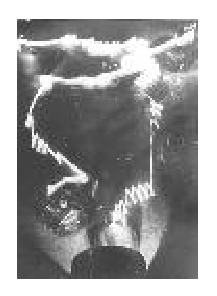
\epsfig{width=3cm,file=notext_ps_logo.eps}
   \end{tabular}
  &
  \hspace{5cm}
  &
  \begin{tabular}{r}
    {\bf Robotics Laboratory}\\
    Stanford University\\
    Stanford, California, USA\\
    \vspace*{2em}\\
    {\bf Robotics Research Laboratory}\\
    University of Southern California\\
    Los Angeles, California, USA\\
    \vspace*{2em}\\
    {\bf Autonomy Laboratory}\\
    Simon Fraser University\\
    Burnaby, British Columbia, Canada\\
  \end{tabular}
\end{tabular}

\vspace{5cm}
\centerline{\huge{Player}}
\vspace{0.5cm}
\centerline{\large{Version \VERSION\ User Manual}}
\vspace{2cm}

\centerline{\large Brian P. Gerkey\\ Richard T. Vaughan\\ Andrew Howard}
\vspace{1cm}
%\centerline{Technical Report IRIS-00-392}
%\centerline{{\tt http://iris.usc.edu/${}_{\tilde{}}$\,irislib}}
%\vspace{1cm}
%\centerline{This report may not contain the most current documentation on}
%\centerline{Player.  For the latest documentation, consult the Player homepage:}
%\centerline{{\tt http://fnord.usc.edu/player}}

\centerline{This document may not contain the most current documentation on}
\centerline{Player.  For the latest documentation, visit the Player/Stage project online:}
\centerline{\HOMEPAGE}

\vspace{3cm}

\centerline{\today}

\tableofcontents
\listoffigures
\listoftables
\newpage

% reset page number to start with 1
\pagenumbering{arabic}
\setcounter{page}{1}
% set the section counter to -1 to make the first section 0
\setcounter{chapter}{-1}
%-----------------------------------------------------------------------------
\chapter{Metadata}
\section{How to Read this Manual}
We know that you are dying to read this entire document, but let us give
you some advice that may save you some time.  If you are only planning
to use Player with the Stage simulator, then you should only need to read
Chapters~\ref{chapt:intro}~and~\ref{chapt:devices} and the manual appropriate
to the language in which you will write your programs.  For example, if
you plan to use the C++ client utilities, then read {\em Player C++ Client
Library Reference Manual}.  The manual that you are currently reading only 
includes documentation for
the C reference client.  Language-specific manuals are provided with the
distribution (and are available from the homepage) for C++, Tcl, and LISP.
Client libraries have also been contributed by users for other languages,
including Python, Java, and Visual C++.  These other client libraries are 
distributed separately; see the contributed clients page for details:\\
\indent \HOMEPAGE{\tt /clients/clients.html}\\
If you intend to use Player with physical hardware, then you should also read 
Chapters~\ref{chapt:running}~\&~\ref{chapt:configfile} and consult
Chapter~\ref{chapt:drivers} in order to familiarize yourself
with the details of connecting the hardware and telling Player
where it is.  If you are interested in modifying an existing
client library or writing your own, then you should also read
Chapters~\ref{chapt:socket}~\&~\ref{chapt:interfaces}, which describe the
message protocol and data formats between client and server.  Finally,
if you want to hack on the server in any way (e.g., add a new device
driver, write your own Player server for a different language/platform),
then you should also read Chapter~\ref{chapt:architecture}, which will
(hopefully) provide all the information that you will need.

\section{A Note on Versions}
This document describes the Player robot server version \VERSION.
It applies to Player versions $>=$ \VERSION\ (at least until we put out
another manual).  Since the previous version, many things have likely
changed.  Thus, this manual does {\em not} apply to older versions
of Player.  You can find an older manual at the Player homepage:
\indent \HOMEPAGE{\tt /doc/doc.html}\\
In addition to providing access to physical hardware, Player is also the
interface to the robot simulators Stage and Gazebo.  The three software
packages evolve independently, and so their version numbers have no
meaningful correspondence (it used to be the case that Player and Stage
versions were matched exactly; this is no longer true).  For information on
which versions of Player and the simulators are compatible, see the online
FAQ:
\indent \HOMEPAGE{\tt /faq.html}\\


%-----------------------------------------------------------------------------
\chapter{Introduction}
\label{chapt:intro}
Player was originally developed by Brian Gerkey and Kasper St\o{}y; the
Stage simulator interface was originally written by Richard T.~Vaughan
and Andrew Howard.  Gazebo and its Player interface were written by Nate
Koenig and Andrew Howard.  Now a part of the larger Player/Stage project,
Player's development is administered by Brian Gerkey, Andrew Howard,
and Richard T.~Vaughan.

Player has historically been developed primarily at the Robotics Research
Lab of the University of Southern California, but the current state of
Player is the result of contributions from a great many developers and
users in unversities, companies, and government labs around the world.
For a list of significant contributors, see:\\
\indent \HOMEPAGE{\tt /credits.html}\\
For a list of known users, see:\\
\indent \HOMEPAGE{\tt /users/users.html}

We have tried to make this documentation as complete as possible.
Hopefully there is sufficient information here for you to use Player
and the provided clients as well as write your clients in your
language of choice. 

What do you like? What do you hate?  How do you use it?
Questions and comments regarding Player should be directed to
our mailing lists:\\
\indent {\tt http://sourceforge.net/mail/?group\_id=42445}\\
and bug / feature request tracker:\\
\indent {\tt http://sourceforge.net/tracker/?group\_id=42445}

\section{License}
\noindent {\bf Player is Free Software, copyrighted by its authors, and
released under the GNU General Public License (GNU GPL):}

\begin{quote}
 This program is free software; you can redistribute it and/or modify
 it under the terms of the GNU General Public License as published by
 the Free Software Foundation; either version 2 of the License, or
 (at your option) any later version.

 This program is distributed in the hope that it will be useful,
 but WITHOUT ANY WARRANTY; without even the implied warranty of
 MERCHANTABILITY or FITNESS FOR A PARTICULAR PURPOSE.  See the
 GNU General Public License for more details.

 You should have received a copy of the GNU General Public License
 along with this program; if not, write to the Free Software
 Foundation, Inc., 59 Temple Place, Suite 330, Boston, MA  02111-1307
 USA
\end{quote}

\noindent {\bf The included Player client libraries are also
simultaneously released under the GNU Lesser General Public License
(GNU LGPL):}

\begin{quote}
This library is free software; you can redistribute it and/or 
modify it under the terms of the GNU Lesser General Public
License as published by the Free Software Foundation; either
version 2.1 of the License, or (at your option) any later version.

This library is distributed in the hope that it will be useful,
but WITHOUT ANY WARRANTY; without even the implied warranty of
MERCHANTABILITY or FITNESS FOR A PARTICULAR PURPOSE.  See the GNU
Lesser General Public License for more details.

You should have received a copy of the GNU Lesser General Public
License along with this library; if not, write to the Free Software
Foundation, Inc., 59 Temple Place, Suite 330, Boston, MA  02111-1307
USA
\end{quote}

\section{Description}
What is Player? Player is a robot device server.  It gives you simple
and complete control over the physical sensors and actuators on your
mobile robot.  When Player is running on your robot, your client control
program connects to it via a standard TCP socket, and communication
is accomplished by the sending and receiving of some of a small set of
simple messages.

Player is designed to be language and platform independent.  Your client
program can run on any machine that has network connectivity to your robot,
and it can be written in any language that can open and control a TCP socket.
Client-side utilities are currently available in C, C++, Tcl, LISP, Java,
and Python.  Further, Player makes no assumptions about how you might want
to structure your robot control programs.  In this way, it is much more
``minimal'' than other robot interfaces.  If you want your client to be a
highly concurrent multi-threaded program, write it like that.  If you like
a simple read-think-act loop, do that.  If you like to control your robot
interactively, try our Tcl client (or write your own client utilities in
your favorite interactive language).

Player is also designed to support virtually any number of clients.  Have you
ever wanted your robots to ``see'' through each others' eyes?  Now they can.
Any client can connect to and read sensor data from (and even write motor
commands to) any instance of Player on any robot.  Aside from distributed
sensing for control, you can also use Player for monitoring of experiments.
For example, while your C++ client controls a robot, you can run a Tk GUI
client elsewhere that shows you current sensor data, and a Python client
that logs data for later analysis.  Also, on-the-fly device requests allow
your clients to gain access to different sensors and actuators as needed
for the task at hand.

In addition to controlling the physical hardware, Player can be used to
interface to the robot simulators Stage and Gazebo.

Last but not least, Player is Free Software.  If you don't like how
something works, change it.  And please send us your patch!

\subsection*{Example of Player Operation}
\begin{figure}[ht]
 \centering
 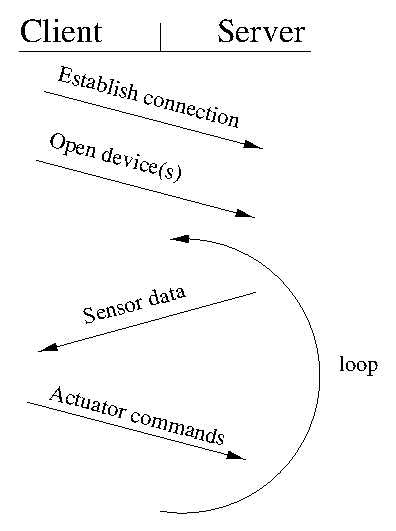
\epsfig{file=exampleuse.eps, height=85mm}
  \caption{{\em Example client/server interaction}}
\label{figure:exampleuse}
 \end{figure} 

As a simple example of the use of Player, consider
Figure~\ref{figure:exampleuse} (note that for clarity, we leave out several
protocol-level interactions).  The server is executing locally on the computer
to which the devices of interest are connected.  In many cases, this computer
is the robot itself, but it could also be, for example, a desktop machine
attached to a SICK laser range-finder.  The client can execute anywhere that
has network connectivity to the machine hosting the server.

First, the client establishes a TCP socket connection to the server.
The client next sends some messages to the server to {\em open} the devices
in which the client is interested.  After that, the server continuously
feeds data from those devices to the client, and the client exerts control
by sending appropriate commands back to the server.  Very simple.


\section{System Requirements}
\label{sect:sysreq}
Player was originally developed on x86/Linux systems, and it is still used
primarily on that platform.  However, with the help of the GNU Autotools
(which rule), Player now builds and runs on most POSIX platforms,
including a number of cross-compiler configurations.  A notable exception
is that Player does {\bf not} run on Windows, and we have {\bf no}
plans to port it to Windows (however, a Cygwin port should be doable;
if you're interested in doing this, let us know).  The current status
of Player for the platforms where it is known to build and run can be
found on the project website. If you have an addition or correction,
please let us know.

To build Player ``out of the box'', you need one of the supported
systems and a recent version of GNU {\tt gcc/g++} (we use some GNU extensions to
C, so other compilers will {\bf not} work).

\section{Getting Player}
\label{sect:gettingplayer}
The Player homepage is:\\
\indent \HOMEPAGE\\
Check there for the latest versions of the server and this
document.

\section{Bugs}
Depite our diligent testing, Player is bound to contain some bugs.
If you manage to break something, or if some aspect of Player's behavior seems 
wrong or non-intuitive, let us know.  

To report a bug or request a feature, {\bf please} do {\bf not} send
mail directly to the developers.  Instead, use the tracking facilities
provided at SourceForge; you can find a link on the Player homepage
(see Section~\ref{sect:gettingplayer}).  Include as much information as
possible, including at least Player version and OS version.  A detailed
description of what happened will enable us (hopefully) to repeat and
analyze the problem.

\section{On the Name Player}
Player was originally named Golem, and the Stage simulator was originally
named Arena.  However, we soon discovered that many,
many, many pieces of robotics-related software already use those names.
So, we had to make a change.  We needed names that capture the now-integral
relationship between the server and simulator, so we chose Player and
Stage, as suggested by a living Englishman, in reference to a
very dead Englishman.

\vspace*{1em}

\noindent
From {\em As You Like It} Act II, Scene 7:
\begin{quote}
  ``All the world's a stage, \\
  And all the men and women merely players: \\
  They have their exits and their entrances; \\
  And one man in his time plays many parts,''\\
\end{quote}

\noindent
From {\em Macbeth} Act V, Scene 5:
\begin{quote}
  ``Life's but a walking shadow, a poor player \\
  That struts and frets his hour upon the stage \\
  And then is heard no more: it is a tale \\
  Told by an idiot, full of sound and fury, \\
  Signifying nothing.''\\
\end{quote}

\section{Acknowledgements}
This work is supported in part by the Intel Foundation, DARPA grant
DABT63-99-1-0015 (MARS), NSF grant ANI-9979457 (SCOWR), DARPA contract
DAAE07-98-C-L028 (TMR), ONR Grants N00014-00-1-0140 and N0014-99-1-0162,
and JPL Contract No. 1216961.

We thank the many developers and users who have contributed so much to the
success of the project, especially: 
Maxim Batalin,
Josh Bers,
Matt Brewer,
Brendan Burns,
Jason Douglas,
Jakob Fredslund,
Ben Grocholsky,
Kim Jinsuck,
Chris Jones,
Boyoon Jung,
Marin Kobilarov,
Nathan Koenig,
James McKenna,
Alex Makarenko,
Andy Martignoni III,
Nik Melchior,
Dave Naffin,
Esben \O{}sterg\aa{}rd,
Dylan Shell,
Gabe Sibley,
Pranav Srivastava,
Kasper St{\o}y,
John Sweeney 
and
Doug Vail.

Thanks also to SourceForge.net for project hosting.

\section{Citations}
If you find Player useful in your work, we would greatly appreciate
your mentioning that fact in papers that you publish.  We have presented
papers on Player in peer-reviewed conferences; the following papers are
the definitive references when citing Player
\cite{VaughanGerkeyHoward03a,GerkeyVaughan01a,GerkeyVaughanHoward03}:
\begin{itemize}
\item Richard~T. Vaughan, Brian~P. Gerkey, and Andrew Howard.
\newblock On device abstractions for portable, reusable robot code.
\newblock In {\em Proc. of the IEEE/RSJ Intl. Conf. on Intelligent Robots and
  Systems (IROS)}, pages 2121--2427, Las Vegas, Nevada, October 2003.
\item
Brian~P. Gerkey, Richard~T. Vaughan, and Andrew Howard.
\newblock {The Player/Stage Project: Tools for Multi-Robot and Distributed
  Sensor Systems}.
\newblock In {\em Proc. of the Intl. Conf. on Advanced Robotics (ICAR)}, pages
  317--323, Coimbra, Portugal, July 2003.
\item
Brian~P. Gerkey, Richard~T. Vaughan, Kasper St\o{}y, Andrew Howard,
Maja~J Matari\'c and Gaurav~S Sukhatme.
\newblock {Most Valuable Player: A Robot Device Server for Distributed
  Control}.
\newblock In {\em Proc. of the IEEE/RSJ Intl. Conf. on Intelligent Robots and
  Systems (IROS)}, pages 1226--1231, Wailea, Hawaii, October 2001.
\end{itemize}
If you have space (and are feeling generous), you can also insert a footnote
similar to the following:
\begin{quote}
Player is freely available under the GNU General Public License from
http://playerstage.sourceforge.net.
\end{quote}
By including such acknowledgements, you do more than feed our egos and further 
our academic careers.  You spread the word about Player, which will bring more
users and developers, as well as please our funders, ensuring that we will
continue to be allowed to hack on the software.
%-----------------------------------------------------------------------------
\chapter{Running Player}
\label{chapt:running}
\section{Building and Installing Player}
System requirements, including platforms on which Player is known to build and
run, are given in Section~\ref{sect:sysreq}.  If you've got one of those
systems and the necessary tools (e.g., {\tt g++}), then the build is
pretty simple.

First, open your source tarball.  Generic instructions are given in 
{\tt INSTALL}, and more information is in {\tt README}.  If you don't feel
like reading those files, the following should suffice:
\begin{verbatim}
  $ ./configure
  $ make
  $ make install
\end{verbatim} %$
Player will be installed in the default location: {\tt /usr/local/}.
{\bf Note that this location differs from older versions, which were
installed in {\tt \$HOME}}.  The {\tt configure} script accepts a number
of options for customizing the build process, including changing the
install location and adding/removing device drivers.  For example,
to change the install location for Player, do:
\begin{verbatim}
  $ ./configure --prefix <path>
\end{verbatim} %$
To see a complete list of such options (e.g., to enable drivers that
aren't built by default), do:
\begin{verbatim}
  $ ./configure --help
\end{verbatim} %$


\section{Command Line Arguments}
\label{sect:commandline}
\begin{table}[ht]
\begin{center}
{\normalsize
\begin{tabularx}{\columnwidth}{|c|X|}
\hline
Argument & Meaning  \\
\hline
-h & Print out usage statement.\\
\hline
-p $<$port$>$ & The Player server should listen on TCP port $<$port$>$.  Default
is {\tt \DEFAULTPORT}. \\
\hline
-s $<$path$>$ & Run Player as a child process under the Stage simulator,
and use memory-mapped IO through the files found in the directory
$<$path$>$ to communicate with the simulator.  Note that \verb+-s+
should only be given manually when you are debugging Player; it is really
intended for use only when Player is spawned by Stage.\\
\hline
-g $<$id$>$ & Connect to a Gazebo simulation engine with the given id.\\
\hline
-r $<$logfile$>$ & Read data from a stored log file instead of real
sensors.  For use with the {\tt readlog} driver. \\
\hline
-d $<$shlib$>$ & The Player server should load the shared object $<$shlib$>$.
This option is generally used to load device drivers from dynamic libraries.
See Section~\ref{sect:shared-lib} for information on building such a library.\\
\hline
-k $<$key$>$ & The Player server should enable authentication.  Clients will
be required to send an authentication request containing $<$key$>$ before Player
will service them.  This option is usually only specified through Stage;
Default is to disable authentication.\\
\hline
$<$configfile$>$ & Player should load and configure device drivers according to
the indicated configuration file.  See Chapter~\ref{chapt:configfile} for
details.\\
\hline
\end{tabularx}
}
\end{center}
\caption{{\em Player command-line arguments}}
\label{table:commandlinefig}
\end{table}

Player is executed as follows:
\begin{verbatim}
  $ player [-p <port>] [-s <path>] [-g <id>] [-r <path>] [-d <shlib>] 
           [-k <key>] [<configfile>]
\end{verbatim}  % $ - I put this here just to stop emacs getting confused. ahoward
The command-line arguments are summarized in
Table~\ref{table:commandlinefig}, and the configuration file syntax is
described in Chapter~\ref{chapt:configfile}.  Note that you can specify
at most one of {\tt -s}, {\tt -g}, or {\tt -r}; if you specify none of
these options, the default is to connect to physical hardware.

\section{Visualization tools}
Once you have Player running, either on a real robot or under Stage, the
first thing that you might want to do is have a look at what your robot
``sees.''  For this purpose, we provide a graphical visualization tool
that we have found most useful in our work.  This tool, {\tt playerv},
can be found in the Player distribution, and is installed alongside {\tt
player} itself in the subdirectory {\tt bin}.  Enjoy.
%-----------------------------------------------------------------------------
\chapter{Device Overview}
\label{chapt:devices}
In Player, we use the notion of a {\em device} in much the same way as most
UNIX systems.  That is, a device is an abstract entity that provides a standard
interface to some service.  Devices behave similarly to files in that they
must be {\em opened} with the correct access mode before use, and {\em closed}
afterward.  Once open, a device can be read from, written to, and configured
(note the similarity to UNIX's {\tt read()}, {\tt write()}, and {\tt ioctl()}),
although not every device supports all three operations.  A conceptual overview
of these device operations is given in Section~\ref{sect:overview-device-ops}.

As in UNIX, devices in Player do {\bf not} have a one-to-one mapping to
physical hardware components, and with good reason.  For example, it so
happens that when retrieving odometry data from the ActivMedia Pioneer 2-DX
robot, one also receives sonar range data.  A client program that only wants
to log the robot's current position should not also receive unwanted sonar
range data; in fact, the client should be completely unaware of the coupling
that exists inside the robot, because it is irrelevant.  In order to present
an intuitive interface to the client, Player controls one physical piece of
hardware, the P2OS microcontroller, but implements two different devices:
{\tt position} and {\tt sonar}.  These two devices can be opened, closed, and
controlled independently, relieving the client of the burden of remembering
details about the internals of the robot.  In addition to making such logical
divisions, the device abstraction allows us to implement more sophisticated
devices that do not simply return sensor data but rather filter or process
it in some way.

Besides controlling different kinds of devices, Player can control multiple
instances of a given kind of device.  For example, if you have 2 SICK laser
range-finders attached to your robot, then you can access both of them through
the use of indices (see Chapter~\ref{chapt:configfile} for how to tell Player
about the devices and Section~\ref{sect:messageformat} for protocol-level
details of indexing).  In fact, all device access is made by index; it just
happens that most of the time, the index is $0$ because there is only one
of each device.

{\bf NOTE:} Player implements {\em no device locking}.  That is, many
clients can have concurrent access to a given device, and they can
concurrently command it.  Player makes no attempt to arbitrate among
the clients, and the command that is actually sent to the device will
be determined by the rate at which the clients are sending commands,
as well as some subtle timing issues.  We purposefully chose not to
implement any device locking, as it results in a more flexible system
in which interesting ideas such as large-scale collaborative control
can be explored (e.g., \cite{GerkeyMataricSukhatme02}).

\section{Device access: data, command, configuration}
\label{sect:overview-device-ops}
\subsection*{Data}
When a client {\tt read}s from a device, the client receives the device's
current data.  For a Player device, the term {\em data} is used to refer to
the salient state of the device.  Of course, this definition is not objective,
and for some devices, there may be more than one reasonable choice at to what
constitutes the {\em data}.  However we find that for most devices we can
readily define the data as the information that is of interest to clients
and that changes (relatively) frequently.  For example, when interacting
with a {\tt sonar} device, which controls an array of sonar tranducers,
the data is simply a list of range readings.  For a {\tt laser} device,
which controls a scanning laser range-finder, the data includes not only the
range readings from the laser but also some current settings of the laser,
such as scanning aperture and angular resolution.  We originally included
only the range readings, but found that the auxillary configuration data is
comparatively small and is in fact required in order to correctly interpret
the range data.  In the same way,  the contents of a device's data will 
in general represent a trade-off between information content and communication
overhead.  Keep in mind that a device's data will usually be transmitted to 
the client at 10Hz (or faster).

\subsection*{Command}
When a client {\tt write}s to a device, the client sends a new command to the
device.  For a Player device, the term {\em command} is used to refer to the
salient {\em controllable} state of the device.  That is, a device's command
will generally include those parameters of the device that are most often
changed in the course of using the device.  For example, when interacting
with a {\tt position} device, which controls a mobile robot, the command
is a set of translational and angular velocities.  Although many other aspects
of the robot are user-configurable, most of the time one need only change
the translational and angular velocities, as they determine the physical
position of the robot, which is the main point of interest.  For a {\tt
speech} device, which controls the a speech synthesizer, we chose to
make the command the ASCII string that is to be synthesized; we believe that
this choice presents a natural interface to the underlying synthesizer.  
Again, command specification will be different for each device, and keep
in mind that a device's command will usually be transmitted to the server
at 10Hz (or faster).

\subsection*{Configuration}
All device interaction that does not qualify as data or command must be
implemented as {\em configuration}.  Whereas data and command are asynchronous,
one-way, (pseudo-)continuous streams, the Player configuration mechanism
provides a synchronous, two-way, request-reply interaction between client and
device.  When a client sends a configuration request to the server, the request
is added to an incoming queue for the appropriate device.  At its leisure,
the device will service the request, generate an appropriate reply and add
it to the device's outgoing queue.  This reply will then be transmitted by
the server to the waiting client.  Thus another distinction of configuration,
as compared with data or command, is that configuration requests and replies
are {\em not} overwritten and so are guaranteed to be received by the device
and the client, respectively\footnote{This is mostly true, at least until the
incoming and/or outgoing queues fill.  If the incoming queue fills, then the
client will be notified by the server (see Section~\ref{sect:messageformat}).
If the outgoing queue fills, then there is not really anthing to do; anyway
this should not happen.}.

In general, any kind of device interaction can be implemented as configuration,
and a device can accept more than one kind of configuration request.  Usually,
configuration is used to assign or query some aspect of the device's state.
For example, when interacting with a {\tt fiducial} device, which finds
special beacons in the environment, there are configuration requests that
can be used to set parameters used in finding and identifying the beacons.
Compared to data and command frequency, configurations are made relatively
rarely; if for a particular device a particular configuration change is made
very often, then the variables being configured should probably be part of
the device's command.


\section{Interfaces vs. Drivers}
In order to support different kinds of hardware, Player makes a
distinction between device {\em interfaces} and device {\em drivers}.
A device interface, such as {\tt ptz}, specifies the format of the data,
command, and configuration interactions that a device allows.  A device
driver, such as {\tt sonyevid30}, specifies how the low-level device
control will be carried out.  In general, more than one driver may support
a given interface\footnote{Conversely, a given driver may support multiple
interfaces; the {\tt amcl} and {\tt segwayrmp} drivers demonstrate this
idea.}, though not all drivers will support all configuration requests.
Thus we extend in Player the analogy of UNIX devices, where, for example,
a wide variety of joysticks all present the same ``joystick'' API to
the programmer.

As an example, consider the two drivers {\tt p2os\_position} and {\tt
rwi\_position}, which control Pioneer mobile robots and RWI mobile robots,
respectively.  They both support the {\tt position} interface and thus
they both accept commands and generate data in the same format, allowing
a client program to treat them identically, ignoring the details of the
underlying hardware.  They also accept configuration requests in the same
format, but not all configuration requests are supported by both drivers.
For example, motor power can be toggled from software with Pioneer robots
but not with RWI robots.  Thus the {\tt p2os\_position} driver supports the
configuration request to toggle motor power, while the {\tt rwi\_position}
driver does not.

All client/server interaction is done by interface, with no reference
to the underlying driver\footnote{This is almost true, except that the driver
name is passed back to the client when a device is opened, just in case the 
client wants to do something driver-specific.}.  So, for example, if
Player has been configured to control a single {\tt position} device with
index 0 and driver {\tt p2os\_position} (see Chapter~\ref{chapt:configfile}
for how specify this information), then the client opens and controls the
$0^{th}$ {\tt position} device.  Player could also be configured to control
a second {\tt position} device with index 1 and driver {\tt rwi\_position};
to access it, the client would open the $1^{st}$ {\tt position} device.

Details on Player's device interfaces and drivers are given in
Chapters~\ref{chapt:interfaces}~\&~\ref{chapt:drivers}, respectively.

\section{Supported Hardware \& Software}
For a table of the currently supported hardware and software, check the
FAQ:\\
\indent \HOMEPAGE{\tt /faq.html}

%-----------------------------------------------------------------------------
\chapter{Configuration Files}
\label{chapt:configfile}
Player needs to know where and how your devices are connected/configured.
For example, if you are controlling a SICK LMS laser, then Player needs
to know to which serial port the laser is connected.  The configuration file
is used to tell Player this information.  

\noindent 
By convention, configuraton files for Player have the extension {\tt .cfg}.
Some example configuraton files are included in the distribution; they are
installed in the subdirectory {\tt config}.

\section{Basic Syntax}
Player's configuration file syntax is very similar to that of Stage (in fact,
they use the same parser and much of the following text is adapted from
the Stage User Manual).  A simple configuration file might look like this:
\begin{quote}
\begin{verbatim}
# The file configures Player to control a Pioneer 2-DX equipped 
# with a gripper and a Sony pan-tilt-zoom camera.

position:0 ( driver "p2os_position" )
sonar:0 ( driver "p2os_sonar" )
gripper:0 ( driver "p2os_gripper" )
ptz:0 ( driver "sonyevid30" )

\end{verbatim}
\end{quote}
This example shows the basic syntactic features of the 
configuration file format: comments, devices, indices, and properties.

Comments are indicated by the \verb'#' symbol; they may be placed
anywhere in the file and continue to the end of the line.  For
example:
\begin{quote}
\begin{verbatim}
# This file configures Player for a Pioneer robot
\end{verbatim}
\end{quote}
Devices are indicated using \verb+interface ( ... )+ entries; each such
entry instantiates a device with interface \verb+interface+.  For example:
\begin{quote}
\begin{verbatim}
position:0 ( ... )
\end{verbatim}
\end{quote}
creates a device with a position interface (e.g., a mobile robot).  The
list of available interfaces is given in Chapter~\ref{chapt:interfaces}.

Player can concurrently control multiple devices with the same interface,
and they are differentiated by indices.  When instantiating a device, its
index is indicated with a colon and number syntax.  For example
\begin{quote}
\begin{verbatim}
ptz:1 ( ... )
\end{verbatim}
\end{quote}
creates a pan-tilt-zoom device that will be identified with index 1.  If the
index is not specified, then an index of 0 is assumed.  Indices need not be
consecutive, but for a given interface, they must be unique.  If multiple 
devices are declared with the same interface and index, then the one that is
declared last will replace the others.

Devices have properties, indicated using \verb'name value' pairs:
\begin{quote}
\begin{verbatim}
position:0 ( driver "p2os_position" port "/dev/ttyS0" )
\end{verbatim}
\end{quote}
This entry creates a position device using the driver \verb+p2os_position+;
that driver will control the underlying robot hardware via the serial port
\verb+/dev/ttyS0+.  Property values can be either numbers (\verb'6665'),
strings (indicated by double quotes \verb'"robot1"') or tuples (indicated
by brackets \verb'[1 1 0]').

There are two special properties, which can be supplied for any device:
\begin{center}
\begin{tabularx}{\columnwidth}{|l|l|c|X|}
\hline
Name & Type & Default & Meaning\\
\hline
{\tt driver} & string & varies & 
Selects which driver will be loaded for this interface.  If no \verb+driver+
is given for a device, then the default driver for the interface will be used.
Default drivers for each interface are given in 
Chapter~\ref{chapt:interfaces}.\\
\hline
{\tt alwayson} & integer & 0 & 
Tells the server to subscribe to the device when the server starts up.
You might use this to frontload startup time for drivers that take a while to
start (e.g., {\tt acts}), to start a device that will never have any direct
clients (e.g., a name service), or for testing a driver without the need to
connect a client.\\
\hline
\end{tabularx}
\end{center}
The remaining driver-specific properties and their defaults are given in
Chapter~\ref{chapt:drivers}.

\section{Defining new device types}

The \verb'define' statement can be used to define new types of devices.
New devices are defined using the syntax:
\begin{quote}
\begin{verbatim}
define newdevice olddevice (...)
\end{verbatim}
\end{quote}
For example, the line:
\begin{quote}
\begin{verbatim}
define pioneer2 position (driver "p2os_position" port "/dev/ttyS0")
\end{verbatim}
\end{quote}
defines a new \verb'pioneer2' device type composed of the
primitive \verb'position' device, appropriately configured for a Pioneer robot
attached to the first serial port.  This device may be instantiated using the 
standard syntax:
\begin{quote}
\begin{verbatim}
pioneer2 ()
\end{verbatim}
\end{quote}

\section{Using include files}

The \verb'include' statement can be used to include device definitions
(or declarations) from another file.  The definitions are included with the 
following syntax:
\begin{quote}
\begin{verbatim}
include "filename"
\end{verbatim}
\end{quote}

\section{Units}

The default units for length and angles are meters and degrees
respectively.  Units may be changed using the following global
properties:

\begin{center}
\begin{tabularx}{.9\textwidth}{|l|l|X|}
\hline
Name & Values & Description \\
\hline
\verb'unit_length' & \verb'"m"', \verb'"cm"', \verb'"mm"'
& Set the unit length to meters, centimeters or millimeters. \\
\hline
\verb'unit_angle' & \verb'"degrees"', \verb'"radians"'
& Set the unit angle to degrees or radians.\\
\hline
\end{tabularx}
\end{center}

\noindent
Be warned that the length specfication applies to the include files as well,
so choose a unit length early and stick to it.

%-----------------------------------------------------------------------------
\chapter{Client/Server Protocol}
\label{chapt:socket}
This section describes the TCP/IP socket interface to the Player server.
Only device-independent information is given here.  For interface-specific
payload formats, see Chapter~\ref{chapt:interfaces}.  For driver-specific
information, see Chapter~\ref{chapt:drivers}.  For language-specific
examples, consult the documentation for the appropriate client library.

\section{A Note on Data Types}
We are about to describe the protocol-level details of the socket
interface to Player.  As such, it is worth making clear two details
regarding data types.  First, the various messages that are sent
between client and server are composed of fields of three different
sizes, as listed in Table~\ref{table:datatypes}.  They may be signed
or unsigned, but they will always be the same size.  

\begin{table}[ht]
\begin{center}
{\small
\begin{tabular}{|c|c|}
\hline
Type & size (in bytes) \\
\hline
{\bf byte/character} & 1 \\
\hline
{\bf short} & 2 \\
\hline
{\bf int} & 4 \\
\hline
\end{tabular}
}
\end{center}
\caption{{\em Data types and their sizes}}
\label{table:datatypes}
\end{table}

The second important detail is that all data on the network is in network
byte-order (big-endian)\footnote{x86 machines are little-endian;
thus clients running on them must byte-swap.}.  
So, before sending a message to the
server, the client must ensure that all multibyte fields 
(i.e., {\bf short}s and {\bf int}s)
are in network byte-order.  Analogously, before interpreting any messages
from the server, the client must ensure that all multibyte fields
are in the native byte-order.
Single characters require no special processing.

Most programming languages provide some method for converting from network 
to native byte-order and back.  For example, in C you can use library functions
like {\tt ntohs()} and {\tt htons()}.  On the other hand, Java handles
byteswapping on data streams automatically, and Tcl offers a choice of
byte-order when using the {\tt binary} command to marshal and demarshal binary
strings.

\section{A Note on Time}
As explained below, Player messages often contain one or more time values,
and it is important that the client be able to interpret them properly.
Player measures time in the same way as many operating systems 
({\tt struct timeval}).
Each time value is represented as two {\bf int}s; one gives the number
of seconds elapsed since the epoch (00:00:00 January 1, 1970) and the other
gives the number of microseconds since the last second elapsed.
Note that the time fields are only ever set by the server when sending
a message to the client; the client should set them to zero when
sending messages to the server.

\section{Connecting to the Server}
First a connection to Player needs to be established. This is done
by creating a TCP socket and connecting to Player on port number\footnote{This 
is the default port; Player can be configured to listen on 
a different port through a command-line option at startup.  See 
Table~\ref{table:commandlinefig}.} \DEFAULTPORT.  Immediately after connection,
Player will respond with a 32-character NULL-terminated string that identifies
its version; if the version string is less than 32 characters in length,
NULL characters will be added to lengthen it.  When Player is interfacing to
real devices, the string will be something like:
\begin{verbatim}
  Player v.1.2.3
\end{verbatim}
When Player is running under Stage, the string will be something like:
\begin{verbatim}
  Player v.1.2.3 (stage)
\end{verbatim}
The client must consume these 32 bytes; whether or not they are used in any
way is up to the client.  After the version string, the server is waiting
for direction from the client.

\section{Message Formats}
\label{sect:messageformat}
Player clients and servers communicate with a simple symmetric message
protocol.  Each message is composed of two parts: a header and a payload.
We now describe the format of the header and of the payloads of
the 4 different message types.

\subsection{Header}
Every Player message has a 32-byte header that contains information
about how to interpret the payload of the message.  The header format
is shown in Table~\ref{table:header}.

\begin{table}[ht]
\begin{center}
{\small
\begin{tabular}{lr}
Byte 0 \hspace{.4\textwidth} & \hspace{.4\textwidth} Byte 31\\
\end{tabular}
\begin{tabular}{|c|c|c|c|c|c|c|c|c|c|}
\hline
{\tt STX} & {\tt type} & {\tt device} & {\tt index} & 
{\tt t\_sec} & {\tt t\_usec} & {\tt ts\_sec} & {\tt ts\_usec} & 
{\tt reserved} & {\tt size}\\
\hline
{\bf short} & {\bf short} & {\bf short} & {\bf short} & 
{\bf int} & {\bf int} & {\bf int} & {\bf int} & {\bf int} & {\bf int} \\
\hline
\end{tabular}
}
\end{center}
\caption{{\em Message header fields and types}}
\label{table:header}
\end{table}

The fields in the header have the following meanings:
\begin{itemize}
\item {\tt STX} - This {\bf short} is a special symbol that signals the start
of a message.  It always has the same value: {\tt 0x5878}.
{\em Remember that this number, like all other {\bf short}s and
{\bf int}s, is transmitted in network byte-order.}

\item {\tt type} - This {\bf short} designates the type of the message to 
follow.  There are 4 message types in the Player protocol. 
Their type codes are given in Table~\ref{table:messagetypes} and they
are described in detail in 
Sections~\ref{sect:datamessages}--\ref{sect:error-responsemessages}.

\begin{table}[ht]
\begin{center}
{\small
\begin{tabular}{|l|l|}
\hline
{\bf Value} & {\bf Meaning} \\
\hline
{\tt 0x0001} & Data message\\
\hline
{\tt 0x0002} & Command message\\
\hline
{\tt 0x0003} & Request message\\
\hline
{\tt 0x0004} & Acknowledgement response message\\
\hline
{\tt 0x0005} & Synchronization message\\
\hline
{\tt 0x0006} & Negative acknowledgment response message\\
\hline
{\tt 0x0007} & Error response message\\
\hline
\end{tabular}
}
\end{center}
\caption{{\em Message type codes}}
\label{table:messagetypes}
\end{table}

\item {\tt device} - This {\bf short} designates the interface to which
the message pertains.  The currently available interface types are given
in Table~\ref{table:devicecodes}.  Descriptions of the interfaces can found
in Chapter~\ref{chapt:interfaces}.

\begin{table}[ht]
\begin{center}
{\small
\begin{tabular}{|l|l|l|}
\hline
{\bf Value} & {\bf Interface} & {\bf Description} \\
\hline
{\tt 0x0001} & {\tt player} & The player server itself \\
\hline
{\tt 0x00FF} & {\tt null} & Null interface \\
\hline
{\tt 0x0002} & {\tt power} & Power subsytem \\
\hline
{\tt 0x0003} & {\tt gripper} & Simple robotic gripper \\
\hline
{\tt 0x0004} & {\tt position} & Mobile robot base \\
\hline
{\tt 0x0005} & {\tt sonar} & Array of fixed acoustic range-finders\\
\hline
{\tt 0x0006} & {\tt laser} & Single-origin scanning range-finder\\
\hline
{\tt 0x0007} & {\tt blobfinder} & Visual color segmentation system\\
\hline
{\tt 0x0008} & {\tt ptz} & Pan-tilt-zoom camera unit \\
\hline
{\tt 0x0009} & {\tt audio} & Fixed-tone generation and detection\\
\hline
{\tt 0x000A} & {\tt fiducial} & Fiducial (e.g., landmark) detector \\
\hline
{\tt 0x000B} & {\tt comms} & General-purpose communication system\\
\hline
{\tt 0x000C} & {\tt speech} & Speech synthesis/recognition system\\
\hline
{\tt 0x000D} & {\tt gps} & Global positioning system\\
\hline
{\tt 0x000E} & {\tt bumper} & Tactile bumper array\\
\hline
{\tt 0x000F} & {\tt truth} & Ground truth (only available in Stage) \\
\hline
{\tt 0x0010} & {\tt idarturret} & Collection of IDAR sensors\\
\hline
{\tt 0x0011} & {\tt idar} & IDAR (Infrared Data and Ranging) sensor\\
\hline
{\tt 0x0012} & {\tt descartes} & The Descartes mobile robot base\\
\hline
{\tt 0x0014} & {\tt dio} & Digitial I/O\\
\hline
{\tt 0x0015} & {\tt aio} & Analog I/O\\
\hline
{\tt 0x0016} & {\tt ir} & Array of fixed infrared range-finders \\
\hline
{\tt 0x0017} & {\tt wifi} & Wireless Ethernet card\\
\hline
{\tt 0x0018} & {\tt waveform} & Raw digital data (e.g., audio) \\
\hline
{\tt 0x0019} & {\tt localize} & Multi-hypothesis localization system\\
\hline
{\tt 0x001A} & {\tt mcom} & Inter-robot stack-based communication\\
\hline
{\tt 0x001B} & {\tt sound} & Play pre-recorded sound files\\
\hline
{\tt 0x001C} & {\tt audiodsp} & Fixed-tone generation and detection\\
\hline
{\tt 0x001D} & {\tt audiomixer} & Control sound levels\\
\hline
{\tt 0x001E} & {\tt position3d} & Robot base that moves in 3D\\
\hline
{\tt 0x001F} & {\tt simulation} & Interface for controlling simulator\\
\hline
{\tt 0x0020} & {\tt service\_adv} & Service discovery \\
\hline
{\tt 0x0021} & {\tt blinkenlight} & Blinking lights\\
\hline
{\tt 0x0022} & {\tt camera} & Camera images \\
\hline
\end{tabular}
}
\end{center}
\caption{{\em Device interface type codes}}
\label{table:devicecodes}
\end{table}

\item {\tt index} - This {\bf short} designates the particular device of type 
{\tt device} to which the message pertains.  For example, if your robot
is equipped with two laser range-finders, an index
of {\tt 0x0000} addresses the first and an index of {\tt 0x0001} addresses
the second.

\item {\tt t\_sec} - {\em (Only set by server)} This {\bf int} is the 
seconds portion of the server's current time.

\item {\tt t\_usec} - {\em (Only set by server)} This {\bf int} is the 
microseconds portion of the server's current time.

\item {\tt ts\_sec} - {\em (Only set by server on data messages)} 
This {\bf int} is the seconds portion of the timestamp supplied by the device
from which the data originated.  It can be interpreted as the time at which
the device ``sensed'' the phenomenom represented by the data.

\item {\tt ts\_usec} - {\em (Only set by server on data messages)} 
This {\bf int} is the microseconds portion of the timestamp supplied by the 
device from which the data originated.  It can be interpreted as the time 
at which the device ``sensed'' the phenomenom represented by the data.

\item {\tt reserved} - This field is reserved for future use.

\item {\tt size} - This {\bf int} is the size in bytes of the payload to
follow (it does not include the size of the header).

\end{itemize}

\subsection{Data Messages}
\label{sect:datamessages}
When read access has been granted for a device, sensor data from that device it
is sent to the client in a data message ({\tt type} {\tt 0x0001}). By default,
the server continuously sends sensor data at 10Hz.  The {\tt device} and {\tt
index} fields designate the device from which the data comes and the {\tt
ts\_sec} and {\tt ts\_usec} fields give the time at which the device generated
the data.  The {\tt t\_sec} and {\tt t\_usec} fields give the server's
current time the payload contains the sensor data, the format of which is
device-specific.  Data formats are given in Chapter~\ref{chapt:interfaces}.

\subsection{Command Messages}
\label{sect:commandmessages}
When write permission has been granted for a device, the client can command
the device by sending a command message ({\tt type} {\tt 0x0002}) to the
server.  The {\tt device} and {\tt index} fields designate the device
for which the command is intended.  The {\tt t\_sec}, {\tt t\_usec},
{\tt ts\_sec}, and {\tt ts\_usec} fields are unused.  The payload
contains the actuator command, the format of which is device-specific.
In the interest of simplifying the protocol, the server does NOT respond
to command messages.  Badly formatted commands and commands to devices for
which write permission was never established will only cause errors to be
printed on the console from which Player was launched.  Command formats are
given in Chapter~\ref{chapt:interfaces}.

\subsection{Request Messages}
\label{sect:requestmessages}
Request messages ({\tt type} {\tt 0x0003}) are sent by the client to the server
to make configuration changes to devices.  Although stricly speaking the device
need not be open in order for the client to configure it, the client should
always open it first to ensure that the configuration change is actually made
(the {\tt player} device is always ``open'').  The {\tt device} and {\tt
index} fields designate the device for which the configuration is intended.
The {\tt t\_sec}, {\tt t\_usec}, {\tt ts\_sec}, and {\tt ts\_usec} fields
are unused.  The payload contains the configuration request, the format of
which is device-specific.  The server will respond to each request message
with an appropriate response message ({\tt type}\  {\tt 0x0004}, {\tt 0x0006},
or {\tt 0x0007}).


\subsection{Acknowledgement Response Messages}
\label{sect:ack-responsemessages}
Acknowledgement response messages ({\tt type} {\tt 0x0004}) are generated as
a result of request messages ({\tt type} {\tt 0x0003}) that were successfully
received, interpreted, and executed by a device.  Acknowledgement response
messages are only sent by the server to the client.  The {\tt device} and {\tt
index} fields designate the device for which the configuration is intended.
The {\tt t\_sec} and {\tt t\_usec} fields give the server's current time;
the {\tt ts\_sec} and {\tt ts\_usec} fields are time at which the device
generated the reply.  The payload contains the response, the format of which
is device-specific.

\subsection{Synchronization Messages}
\label{sect:synchmessage}
After each round of data, the server sends a single synchronization message
(type {\tt 0x0005}), with a zero-length body.  This message lets the client 
know that all data for this cycle has been sent.  The synchronization message 
is sent even when no data was sent, as can occur if the client is using one 
of the data delivery modes that only send {\em new} data.

\subsection{Negative Acknowledgement Response Messages}
\label{sect:nack-responsemessages}
Negative acknowledgement response messages ({\tt type} {\tt 0x0006})
are generated as a result of request messages ({\tt type} {\tt 0x0003})
that were successfully received by a device, but which could not be properly
interpreted or executed.  Negative acknowledgement response messages are only
sent by the server to the client.  The {\tt device} and {\tt index} fields
designate the device for which the configuration is intended.  The {\tt t\_sec}
and {\tt t\_usec} fields give the server's current time; the {\tt ts\_sec}
and {\tt ts\_usec} fields are time at which the device generated the reply.
The payload contains the response, the format of which is device-specific.

\subsection{Error Acknowledgement Response Messages}
\label{sect:error-responsemessages}
Error acknowledgement response messages ({\tt type} {\tt 0x0007}) are
generated as a result of request messages ({\tt type} {\tt 0x0003}) that
could not be handed off to the target device, usually because the device's
incoming configuration queue is full.  Error acknowledgement response messages
are only sent by the server to the client.  The {\tt device} and {\tt index}
fields designate the device for which the configuration is intended.  The {\tt
t\_sec} and {\tt t\_usec} fields give the server's current time; the {\tt
ts\_sec} and {\tt ts\_usec} fields are unused.  The payload will be empty.
%-----------------------------------------------------------------------------
\chapter{Device Interfaces}
\label{chapt:interfaces}

In this chapter, we define the various interface-specific payload formats.
The Player protocol itself is described in Chapter~\ref{chapt:socket}.
Although this section is generally up-to-date, the best place to look
for the ``real'' message formats is in the header file 
{\tt player.h}; that file defines the C {\tt struct}s that
are manipulated by Player and the various device drivers.

%%%%%%%%%%%%%%%%%%%%%%%%%%%%%%%%%%%%%%%%%%%%%%%%%%%%%%%%%%%%%%%%%%%%%%%%%%%%%%%
% player
%%%%%%%%%%%%%%%%%%%%%%%%%%%%%%%%%%%%%%%%%%%%%%%%%%%%%%%%%%%%%%%%%%%%%%%%%%%%%%%
\newinterface
\input{interfaces/Player}

%%%%%%%%%%%%%%%%%%%%%%%%%%%%%%%%%%%%%%%%%%%%%%%%%%%%%%%%%%%%%%%%%%%%%%%%%%%%%%%
% null
%%%%%%%%%%%%%%%%%%%%%%%%%%%%%%%%%%%%%%%%%%%%%%%%%%%%%%%%%%%%%%%%%%%%%%%%%%%%%%%
\newinterface
\section{null} \label{sect:null}

\subsection*{Synopsis}

The {\tt null} interface produces no data, and accepts no commands or
configuration requests.  It is the Player analogue to {\tt /dev/null}.



%%%%%%%%%%%%%%%%%%%%%%%%%%%%%%%%%%%%%%%%%%%%%%%%%%%%%%%%%%%%%%%%%%%%%%%%%%%%%%%
% aio
%%%%%%%%%%%%%%%%%%%%%%%%%%%%%%%%%%%%%%%%%%%%%%%%%%%%%%%%%%%%%%%%%%%%%%%%%%%%%%%
\newinterface
\input{interfaces/aio}

%%%%%%%%%%%%%%%%%%%%%%%%%%%%%%%%%%%%%%%%%%%%%%%%%%%%%%%%%%%%%%%%%%%%%%%%%%%%%%%
% audio
%%%%%%%%%%%%%%%%%%%%%%%%%%%%%%%%%%%%%%%%%%%%%%%%%%%%%%%%%%%%%%%%%%%%%%%%%%%%%%%
\newinterface
\input{interfaces/audio}

%%%%%%%%%%%%%%%%%%%%%%%%%%%%%%%%%%%%%%%%%%%%%%%%%%%%%%%%%%%%%%%%%%%%%%%%%%%%%%%
% audiodsp
%%%%%%%%%%%%%%%%%%%%%%%%%%%%%%%%%%%%%%%%%%%%%%%%%%%%%%%%%%%%%%%%%%%%%%%%%%%%%%%
\newinterface
\input{interfaces/audiodsp}

%%%%%%%%%%%%%%%%%%%%%%%%%%%%%%%%%%%%%%%%%%%%%%%%%%%%%%%%%%%%%%%%%%%%%%%%%%%%%%%
% audiomixer
%%%%%%%%%%%%%%%%%%%%%%%%%%%%%%%%%%%%%%%%%%%%%%%%%%%%%%%%%%%%%%%%%%%%%%%%%%%%%%%
\newinterface
\input{interfaces/audiomixer}

%%%%%%%%%%%%%%%%%%%%%%%%%%%%%%%%%%%%%%%%%%%%%%%%%%%%%%%%%%%%%%%%%%%%%%%%%%%%%%%
% blobfinder
%%%%%%%%%%%%%%%%%%%%%%%%%%%%%%%%%%%%%%%%%%%%%%%%%%%%%%%%%%%%%%%%%%%%%%%%%%%%%%%
\newinterface
\input{interfaces/blobfinder}

%%%%%%%%%%%%%%%%%%%%%%%%%%%%%%%%%%%%%%%%%%%%%%%%%%%%%%%%%%%%%%%%%%%%%%%%%%%%%%%
% bumper
%%%%%%%%%%%%%%%%%%%%%%%%%%%%%%%%%%%%%%%%%%%%%%%%%%%%%%%%%%%%%%%%%%%%%%%%%%%%%%%
\newinterface
\input{interfaces/bumper}

%%%%%%%%%%%%%%%%%%%%%%%%%%%%%%%%%%%%%%%%%%%%%%%%%%%%%%%%%%%%%%%%%%%%%%%%%%%%%%%
% comms
%%%%%%%%%%%%%%%%%%%%%%%%%%%%%%%%%%%%%%%%%%%%%%%%%%%%%%%%%%%%%%%%%%%%%%%%%%%%%%%
\newinterface
\input{interfaces/comms}

%%%%%%%%%%%%%%%%%%%%%%%%%%%%%%%%%%%%%%%%%%%%%%%%%%%%%%%%%%%%%%%%%%%%%%%%%%%%%%%
% camera
%%%%%%%%%%%%%%%%%%%%%%%%%%%%%%%%%%%%%%%%%%%%%%%%%%%%%%%%%%%%%%%%%%%%%%%%%%%%%%%
\newinterface
\input{interfaces/camera}

%%%%%%%%%%%%%%%%%%%%%%%%%%%%%%%%%%%%%%%%%%%%%%%%%%%%%%%%%%%%%%%%%%%%%%%%%%%%%%%
% dio
%%%%%%%%%%%%%%%%%%%%%%%%%%%%%%%%%%%%%%%%%%%%%%%%%%%%%%%%%%%%%%%%%%%%%%%%%%%%%%%
\newinterface
\input{interfaces/dio}

%%%%%%%%%%%%%%%%%%%%%%%%%%%%%%%%%%%%%%%%%%%%%%%%%%%%%%%%%%%%%%%%%%%%%%%%%%%%%%%
% fiducial
%%%%%%%%%%%%%%%%%%%%%%%%%%%%%%%%%%%%%%%%%%%%%%%%%%%%%%%%%%%%%%%%%%%%%%%%%%%%%%%
\newinterface
\input{interfaces/fiducial}

%%%%%%%%%%%%%%%%%%%%%%%%%%%%%%%%%%%%%%%%%%%%%%%%%%%%%%%%%%%%%%%%%%%%%%%%%%%%%%%
% gps
%%%%%%%%%%%%%%%%%%%%%%%%%%%%%%%%%%%%%%%%%%%%%%%%%%%%%%%%%%%%%%%%%%%%%%%%%%%%%%%
\newinterface
\input{interfaces/gps}

%%%%%%%%%%%%%%%%%%%%%%%%%%%%%%%%%%%%%%%%%%%%%%%%%%%%%%%%%%%%%%%%%%%%%%%%%%%%%%%
% gripper
%%%%%%%%%%%%%%%%%%%%%%%%%%%%%%%%%%%%%%%%%%%%%%%%%%%%%%%%%%%%%%%%%%%%%%%%%%%%%%%
\newinterface
\input{interfaces/gripper}

%%%%%%%%%%%%%%%%%%%%%%%%%%%%%%%%%%%%%%%%%%%%%%%%%%%%%%%%%%%%%%%%%%%%%%%%%%%%%%%
% ir
%%%%%%%%%%%%%%%%%%%%%%%%%%%%%%%%%%%%%%%%%%%%%%%%%%%%%%%%%%%%%%%%%%%%%%%%%%%%%%%
\newinterface
\input{interfaces/ir}

%%%%%%%%%%%%%%%%%%%%%%%%%%%%%%%%%%%%%%%%%%%%%%%%%%%%%%%%%%%%%%%%%%%%%%%%%%%%%%%
% laser
%%%%%%%%%%%%%%%%%%%%%%%%%%%%%%%%%%%%%%%%%%%%%%%%%%%%%%%%%%%%%%%%%%%%%%%%%%%%%%%
\newinterface
\input{interfaces/laser}

%%%%%%%%%%%%%%%%%%%%%%%%%%%%%%%%%%%%%%%%%%%%%%%%%%%%%%%%%%%%%%%%%%%%%%%%%%%%%%%
% localization
%%%%%%%%%%%%%%%%%%%%%%%%%%%%%%%%%%%%%%%%%%%%%%%%%%%%%%%%%%%%%%%%%%%%%%%%%%%%%%%
\newinterface
\input{interfaces/localize}

%%%%%%%%%%%%%%%%%%%%%%%%%%%%%%%%%%%%%%%%%%%%%%%%%%%%%%%%%%%%%%%%%%%%%%%%%%%%%%%
% mcom
%%%%%%%%%%%%%%%%%%%%%%%%%%%%%%%%%%%%%%%%%%%%%%%%%%%%%%%%%%%%%%%%%%%%%%%%%%%%%%%
\newinterface
\input{interfaces/mcom}

%%%%%%%%%%%%%%%%%%%%%%%%%%%%%%%%%%%%%%%%%%%%%%%%%%%%%%%%%%%%%%%%%%%%%%%%%%%%%%%
% motor
%%%%%%%%%%%%%%%%%%%%%%%%%%%%%%%%%%%%%%%%%%%%%%%%%%%%%%%%%%%%%%%%%%%%%%%%%%%%%%%
\newinterface
\input{interfaces/motor}

%%%%%%%%%%%%%%%%%%%%%%%%%%%%%%%%%%%%%%%%%%%%%%%%%%%%%%%%%%%%%%%%%%%%%%%%%%%%%%%
% position
%%%%%%%%%%%%%%%%%%%%%%%%%%%%%%%%%%%%%%%%%%%%%%%%%%%%%%%%%%%%%%%%%%%%%%%%%%%%%%%
\newinterface
\input{interfaces/position}

%%%%%%%%%%%%%%%%%%%%%%%%%%%%%%%%%%%%%%%%%%%%%%%%%%%%%%%%%%%%%%%%%%%%%%%%%%%%%%%
% position2d
%%%%%%%%%%%%%%%%%%%%%%%%%%%%%%%%%%%%%%%%%%%%%%%%%%%%%%%%%%%%%%%%%%%%%%%%%%%%%%%
\newinterface
\input{interfaces/position2d}

%%%%%%%%%%%%%%%%%%%%%%%%%%%%%%%%%%%%%%%%%%%%%%%%%%%%%%%%%%%%%%%%%%%%%%%%%%%%%%%
% position3d
%%%%%%%%%%%%%%%%%%%%%%%%%%%%%%%%%%%%%%%%%%%%%%%%%%%%%%%%%%%%%%%%%%%%%%%%%%%%%%%
\newinterface
\input{interfaces/position3d}

%%%%%%%%%%%%%%%%%%%%%%%%%%%%%%%%%%%%%%%%%%%%%%%%%%%%%%%%%%%%%%%%%%%%%%%%%%%%%%%
% power
%%%%%%%%%%%%%%%%%%%%%%%%%%%%%%%%%%%%%%%%%%%%%%%%%%%%%%%%%%%%%%%%%%%%%%%%%%%%%%%
\newinterface
\input{interfaces/power}

%%%%%%%%%%%%%%%%%%%%%%%%%%%%%%%%%%%%%%%%%%%%%%%%%%%%%%%%%%%%%%%%%%%%%%%%%%%%%%%
% ptz
%%%%%%%%%%%%%%%%%%%%%%%%%%%%%%%%%%%%%%%%%%%%%%%%%%%%%%%%%%%%%%%%%%%%%%%%%%%%%%%
\newinterface
\input{interfaces/ptz}

%%%%%%%%%%%%%%%%%%%%%%%%%%%%%%%%%%%%%%%%%%%%%%%%%%%%%%%%%%%%%%%%%%%%%%%%%%%%%%%
% simulation
%%%%%%%%%%%%%%%%%%%%%%%%%%%%%%%%%%%%%%%%%%%%%%%%%%%%%%%%%%%%%%%%%%%%%%%%%%%%%%%
\newinterface
\input{interfaces/simulation}

%%%%%%%%%%%%%%%%%%%%%%%%%%%%%%%%%%%%%%%%%%%%%%%%%%%%%%%%%%%%%%%%%%%%%%%%%%%%%%%
% sonar
%%%%%%%%%%%%%%%%%%%%%%%%%%%%%%%%%%%%%%%%%%%%%%%%%%%%%%%%%%%%%%%%%%%%%%%%%%%%%%%
\newinterface
\input{interfaces/sonar}

%%%%%%%%%%%%%%%%%%%%%%%%%%%%%%%%%%%%%%%%%%%%%%%%%%%%%%%%%%%%%%%%%%%%%%%%%%%%%%%
% sound
%%%%%%%%%%%%%%%%%%%%%%%%%%%%%%%%%%%%%%%%%%%%%%%%%%%%%%%%%%%%%%%%%%%%%%%%%%%%%%%
\newinterface
\input{interfaces/sound}

%%%%%%%%%%%%%%%%%%%%%%%%%%%%%%%%%%%%%%%%%%%%%%%%%%%%%%%%%%%%%%%%%%%%%%%%%%%%%%%
% speech
%%%%%%%%%%%%%%%%%%%%%%%%%%%%%%%%%%%%%%%%%%%%%%%%%%%%%%%%%%%%%%%%%%%%%%%%%%%%%%%
\newinterface
\input{interfaces/speech}

%%%%%%%%%%%%%%%%%%%%%%%%%%%%%%%%%%%%%%%%%%%%%%%%%%%%%%%%%%%%%%%%%%%%%%%%%%%%%%%
% truth
%%%%%%%%%%%%%%%%%%%%%%%%%%%%%%%%%%%%%%%%%%%%%%%%%%%%%%%%%%%%%%%%%%%%%%%%%%%%%%%
\newinterface
\input{interfaces/truth}

%%%%%%%%%%%%%%%%%%%%%%%%%%%%%%%%%%%%%%%%%%%%%%%%%%%%%%%%%%%%%%%%%%%%%%%%%%%%%%%
% waveform
%%%%%%%%%%%%%%%%%%%%%%%%%%%%%%%%%%%%%%%%%%%%%%%%%%%%%%%%%%%%%%%%%%%%%%%%%%%%%%%
\newinterface
\input{interfaces/waveform}

%%%%%%%%%%%%%%%%%%%%%%%%%%%%%%%%%%%%%%%%%%%%%%%%%%%%%%%%%%%%%%%%%%%%%%%%%%%%%%%
% wifi
%%%%%%%%%%%%%%%%%%%%%%%%%%%%%%%%%%%%%%%%%%%%%%%%%%%%%%%%%%%%%%%%%%%%%%%%%%%%%%%
\newinterface
\input{interfaces/wifi}

%%%%%%%%%%%%%%%%%%%%%%%%%%%%%%%%%%%%%%%%%%%%%%%%%%%%%%%%%%%%%%%%%%%%%%%%%%%%%%%
% bps
%%%%%%%%%%%%%%%%%%%%%%%%%%%%%%%%%%%%%%%%%%%%%%%%%%%%%%%%%%%%%%%%%%%%%%%%%%%%%%%
%\newinterface
%\section{{\tt bps} {\bf (Unfinished)}}

\subsection*{Overview}

The {\tt bps} device ({\bf b}eacon-based {\bf p}ositioning {\bf
s}ystem) determines the current global pose (position and
orientation) of the robot.  This pose is determined by combining
odometric measurements from the {\tt position} device with beacon
measurements from the {\tt laserbeacon} device.  Beacons must be
pre-placed at known locations, and these locations must be provided to
the {\tt bps} device via a configuration request.

Note that the {\tt bps} device is still experimental; while the external
interface is now more-or-less fixed, the internal structure is likely
to evolve.

\subsection*{Data}

The {\tt bps} device returns an estimate of the current position and
orientation of the robot.  The format for the data packet is given in
Table~\ref{table:bps_data}.

\begin{table}[ht]
\begin{center}
\begin{tabularx}{\columnwidth}{|l|l|X|}
\hline
Field & Type & Meaning\\
\hline
{\tt px} & {\bf int} & Current X position (mm)\\
{\tt py} & {\bf int} & Current Y position (mm)\\
{\tt pa} & {\bf int} & Current orientation (degrees)\\
{\tt ux} & {\bf int} & Current X uncertainty (mm)\\
{\tt uy} & {\bf int} & Current Y uncertainty (mm)\\
{\tt ua} & {\bf int} & Current orientation uncertainty (degrees)\\
{\tt reserved} & & Reserved\\
\hline
\end{tabularx}
\end{center}
\caption{{\em Format of data from the {\tt bps} device.}}
\label{table:bps_data}
\end{table}

\subsection*{Command}
The {\tt bps} device accepts no commands.

\subsection*{Configuration}

The {\tt bps} device accepts two configuration requests: 
{\tt setbeacon} and {\tt setlaser}.
The {\tt setbeacon} request adds a beacon to the robot's internal map;
the identity, position and orientation of the beacon must be supplied.
Note that beacons must be {\em unique}: i.e. no two beacons in the
environment can have the same identity.
The {\tt setlaser} request sets the pose of the laser in the
robot-centered coordinate system.  If the laser is placed near the
center of the robot, this offset can usually be ignored.
The format of the configuration request packets is shown in
Table~\ref{table:bps_config}.

\begin{table}[ht]
\begin{center}
\begin{tabularx}{\columnwidth}{|l|l|l|X|}
\hline
Request & Field & Type & Meaning \\
\hline
{\tt setbeacon} & {\tt subtype} & {\bf unsigned byte} & Request sub-type; must be 2. \\
                & {\tt id} & {\bf unsigned byte} & Beacon id. \\
                & {\tt px} & {\bf int} & Beacon X position (mm). \\
                & {\tt py} & {\bf int} & Beacon Y position (mm). \\
                & {\tt pa} & {\bf int} & Beacon orientation (degrees). \\
                & {\tt ux} & {\bf int} & Beacon X uncertainty (mm). \\
                & {\tt uy} & {\bf int} & Beacon Y uncertainty (mm). \\
                & {\tt ua} & {\bf int} & Beacon orientation uncertainty (degrees). \\
\hline
{\tt setlaser} & {\tt subtype} & {\bf unsigned byte} & Request sub-type; must be 3. \\
               & {\tt px} & {\bf int} & Laser X position (mm). \\
               & {\tt py} & {\bf int} & Laser Y position (mm). \\
               & {\tt pa} & {\bf int} & Laser orientation (degrees). \\
\hline
\end{tabularx}
\end{center}
\caption{{\em Format of the configuration requests from the {\tt bps} device.}}
\label{table:bps_config}
\end{table}


%%%%%%%%%%%%%%%%%%%%%%%%%%%%%%%%%%%%%%%%%%%%%%%%%%%%%%%%%%%%%%%%%%%%%%%%%%%%%%%
% idarturret
%%%%%%%%%%%%%%%%%%%%%%%%%%%%%%%%%%%%%%%%%%%%%%%%%%%%%%%%%%%%%%%%%%%%%%%%%%%%%%%
%\newinterface
%\section{{\tt idarturret}}
\subsection*{Synopsis}
The {\tt idarturret} interface provides access to a collection of IDAR
(Infrared Data And Ranging) sensors.

\subsection*{Drivers}
The {\tt idarturret} interface is only supported by Stage.

\subsection*{Data}
The {\tt idarturret} interface returns no data.

\subsection*{Command}
The {\tt idarturret} interface accepts no commands.

\subsection*{Configuration}
The {\tt idarturret} interface cannot be configured.


%%%%%%%%%%%%%%%%%%%%%%%%%%%%%%%%%%%%%%%%%%%%%%%%%%%%%%%%%%%%%%%%%%%%%%%%%%%%%%%
% idar
%%%%%%%%%%%%%%%%%%%%%%%%%%%%%%%%%%%%%%%%%%%%%%%%%%%%%%%%%%%%%%%%%%%%%%%%%%%%%%%
%\newinterface
%\section{{\tt idar}}
\subsection*{Synopsis}
The {\tt idar} interface provides access to an IDAR (Infrared Data And
Ranging) sensors.

\subsection*{Drivers}
The {\tt idar} interface is only supported by Stage.

\subsection*{Data}
The {\tt idar} interface returns no data.

\subsection*{Command}
The {\tt idar} interface accepts no commands.

\subsection*{Configuration}
The {\tt idar} interface cannot be configured.


%%%%%%%%%%%%%%%%%%%%%%%%%%%%%%%%%%%%%%%%%%%%%%%%%%%%%%%%%%%%%%%%%%%%%%%%%%%%%%%
% descartes
%%%%%%%%%%%%%%%%%%%%%%%%%%%%%%%%%%%%%%%%%%%%%%%%%%%%%%%%%%%%%%%%%%%%%%%%%%%%%%%
%\newinterface
%\section{{\tt descartes}}
\subsection*{Synopsis}
The {\tt descartes} interface provides access to an HRL Descartes holonomic
robot base, with bumpers.

\subsection*{Drivers}
The {\tt descartes} interface is only supported by Stage.

\subsection*{Data}
The {\tt descartes} interface returns data regarding the current state of the
Descartes base; the format is given in Table~\ref{table:descartesdata}.

\begin{table}[ht]
\begin{center}
{\small \begin{tabular}{|l|l|l|}
\hline
Field & Type & Meaning\\
\hline
{\tt xpos} & {\bf int} & X position (in mm)\\
\hline
{\tt ypos} & {\bf int} & Y position (in mm)\\
\hline
{\tt heading} & {\bf short} & Heading (in degrees)\\
\hline
{\tt bumpers} & array of 2 {\bf unsigned byte}s & State of bumpers (boolean)\\
\hline
\end{tabular}}
\end{center}
\caption{{\em Format of data from the {\tt descartes} interface 
(12 bytes total).}}
\label{table:descartesdata}
\end{table}

\subsection*{Command}
The {\tt descartes} interface accepts no commands.

\subsection*{Configuration}
The {\tt descartes} interface cannot be configured.


%%%%%%%%%%%%%%%%%%%%%%%%%%%%%%%%%%%%%%%%%%%%%%%%%%%%%%%%%%%%%%%%%%%%%%%%%%%%%%%
% mote
%%%%%%%%%%%%%%%%%%%%%%%%%%%%%%%%%%%%%%%%%%%%%%%%%%%%%%%%%%%%%%%%%%%%%%%%%%%%%%%
%\newinterface
%\input(interfaces/mote}


%-----------------------------------------------------------------------------


\chapter{Device Drivers}
\label{chapt:drivers}
In this chapter we describe the device drivers included in Player.
For each driver, the supported interfaces, configuration requests, and
configuration file options are given.  The syntax for specifying configuration
file options is given in Chapter~\ref{chapt:configfile}.

\newdriverex{acts}{\gerkey}
\subsection*{Synopsis}
ACTS is a fast color segmentation system written by Paul Rybski and sold
by ActivMedia; see:\\
\indent {\tt http://www.activrobots.com}\\
After training, ACTS finds colored blobs in a single camera image.
Player's {\tt acts} driver provides access to ACTS.


\subsection*{Interfaces}

\noindent Supported interfaces:
\begin{itemize}
\item {\tt blobfinder}
\end{itemize}

\noindent Required devices:
\begin{itemize}
\item None.
\end{itemize}

\noindent Supported configuration requests:
\begin{itemize}
\item None.
\end{itemize}


\subsection*{Configuration file options}
Note: In the table below, a default value of (none) indicates that the
associated option will not be passed to ACTS.  As a result, ACTS's own
internal default for that parameter will be used.  Consult the ACTS manual
to determine what those defaults are.

\begin{center}
{\small \begin{tabularx}{\columnwidth}{|l|l|c|X|}
\hline
Name & Type & Default & Meaning\\
\hline
{\tt path} & string & {\tt ""} & Path to the ACTS executable (leave empty to
search the user's PATH for {\tt acts}).\\

{\tt configfile} & string & {\tt "/usr/local/acts/actsconfig"} & Path to the
ACTS configuration file to be used.\\

{\tt version} & string & {\tt "2.0"} & The version of ACTS in use (should be
{\tt "1.0"}, {\tt "1.2"}, or {\tt "2.0"}).\\

{\tt width} & integer & {\tt 160} & Width of the camera image (in pixels).\\

{\tt height} & integer & {\tt 120} & Height of the camera image (in pixels).\\

{\tt pixels} & integer & (none) & Minimum area required to call a blob a blob 
(in pixels).\\

{\tt port} & integer & {\tt 5001} & TCP port by which Player should connect to
ACTS.\\

{\tt fps} & integer & (none) & Frame per second of the camera.\\

{\tt drivertype} & string & (none) & Type of framegrabber driver in use (e.g.,
{\tt "bttv"}, {\tt "bt848"}, {\tt "matrox"}).\\

{\tt invert} & integer & (none) & Is the camera inverted?\\

{\tt devicepath} & string & (none) & Path to the device file for the
framegrabber (e.g., {\tt "/dev/fg0"}).\\

{\tt channel} & integer & (none) & Which channel to select on the
framegrabber.\\

{\tt norm} & string & (none) & Normalization??\\

{\tt pxc200} & integer & (none) & Is the framegrabber a PXC200?\\

{\tt brightness} & float & (none) & Brightness level??\\

{\tt contrast} & float & (none) & Contrast level??\\
\hline
\end{tabularx}}
\end{center}

\subsection*{Notes}

\begin{itemize}
\item The {\tt acts} driver supports ACTS versions 1.0, 1.2, and 2.0.
\item PXC200 framegrabbers, when accessed through the {\tt bttv} module,
may cause the machine to hang.  A workaround is to first read a frame from
a framegrabber channel on which there is no video signal, and then start
reading from the right channel.  (This problem is unrelated to Player's {\tt
acts} driver)
\end{itemize}


\newdriverex{acoustics}{\nate}
% acoustics

\subsection*{Synopsis}

TODO

\subsection*{Interfaces}

\noindent Supported interfaces:

\begin{itemize}
\item {\tt audiodsp}
\end{itemize}

\noindent Required devices:
\begin{itemize}
\item None.
\end{itemize}

\noindent Supported configuration requests:
\begin{itemize}
\item TODO
\end{itemize}


\subsection*{Configuration file options}

TODO

\subsection*{Notes}

TODO


\newdriverex{amcl}{\ahoward,\boyoon}
%\section{\tt amcl}
%\label{sect:amcl_driver}

\subsection*{Synopsis}

The {\tt amcl} driver implements the Adaptive Monte-Carlo
Localization algorithm described by Fox \cite{fox01a}.
%
At the conceptual level, the {\tt amcl} driver maintains a
probability distribution over the set of all possible robot poses, and
updates this distribution using data from odometry, sonar and/or laser
range-finders.  The driver also requires a pre-defined map of the
environment against which to compare observed sensor values.
%
At the implementation level, the {\tt amcl} driver represents
the probability distribution using a particle filter.  The filter is
``adaptive'' because it dynamically adjusts the number of particles in
the filter: when the robot's pose is highly uncertain, the number of
particles is increased; when the robot's pose is well determined, the
number of particles is decreased.  The driver is therefore able make a
trade-off between processing speed and localization accuracy.

As an example, consider the sequence of images shown in Figure
\ref{fig.amcl.example}.  This sequence shows the filter converging
from an initial configuration in which the pose of the robot is
entirely unknown to a final configuration in which the pose of the
robot is well determined.  At the same time, the number of particles
in the filter decreases from 100,000 to less than 100.

% What it will do
The {\tt amcl} driver has the some of the usual features --
and failures -- associated with simple Monte-Carlo Localization
techniques:
  \begin{itemize}
  \item If the robot's initial pose is specified as being completely
  unknown, the driver's estimate will usually converge to correct
  pose.  This assumes that the particle filter starts with a large
  number of particles (to cover the space of possible poses), and that
  the robot is driven some distance through the environment (to
  collect observations).
  \item If the robot's initial pose is specified accurately, but
  incorrectly, or if the robot becomes lost (e.g., by picking it up
  and replacing it elsewhere) the driver's estimate will not converge
  on the correct pose.  Such situations require the use of more
  advanced techniques that have not yet been implemented (see
  \cite{thrun01a}, for example).
  \end{itemize}
The {\tt amcl} driver also has some slightly unusual temporal
behavior:
  \begin{itemize}
  \item When the number of particles in the filter is large, data may
  arrive from the sensors faster than it can be processed.  When this
  happens, data is queued up for later processing, but the driver
  continues to generate an up-to-date estimate for the robot pose.
  Thus, for example, at time $t = 10$~sec, the driver may have only
  processed sensor readings up until time $t = 5$~sec, but will
  nevertheless generate an estimate (prediction) of where the robot is
  at $t = 10$~sec.  The adaptive nature of the algorithm more-or-less
  guarantees that the driver will eventual ``catch up'': as more
  sensor readings are processed, the number of particles will
  generally decrease, and the sensor update step of the algorithm will
  run faster.
  \end{itemize}

\begin{figure*}[t]
\begin{center}
\begin{tabular}{cc}

\epsfig{height=4cm,file=drivers/amcl-phe200-0010.eps} &
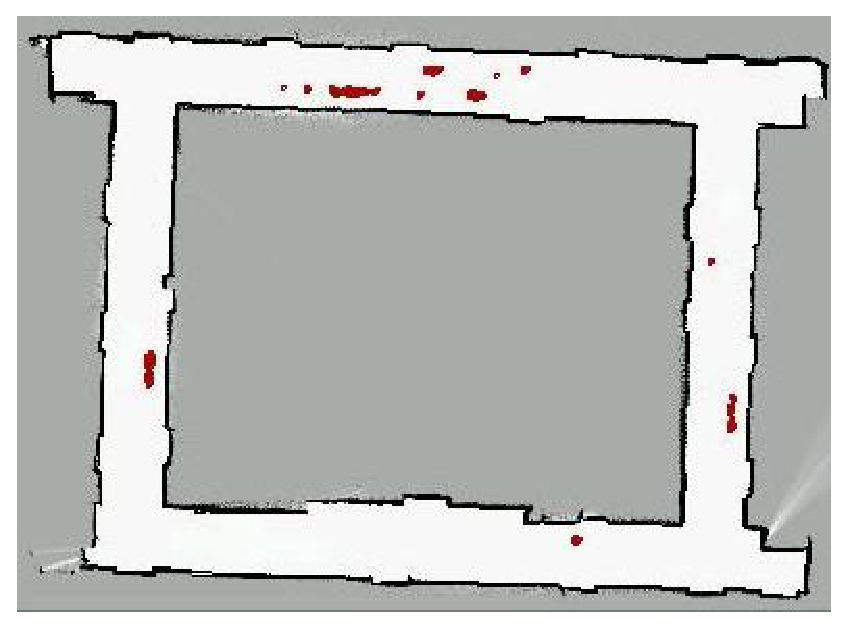
\epsfig{height=4cm,file=drivers/amcl-phe200-0400.eps} \\
$t = 10$~sec, $\approx 100,000$ particles & $t = 10$~sec, $\approx 1,000$ particles \\
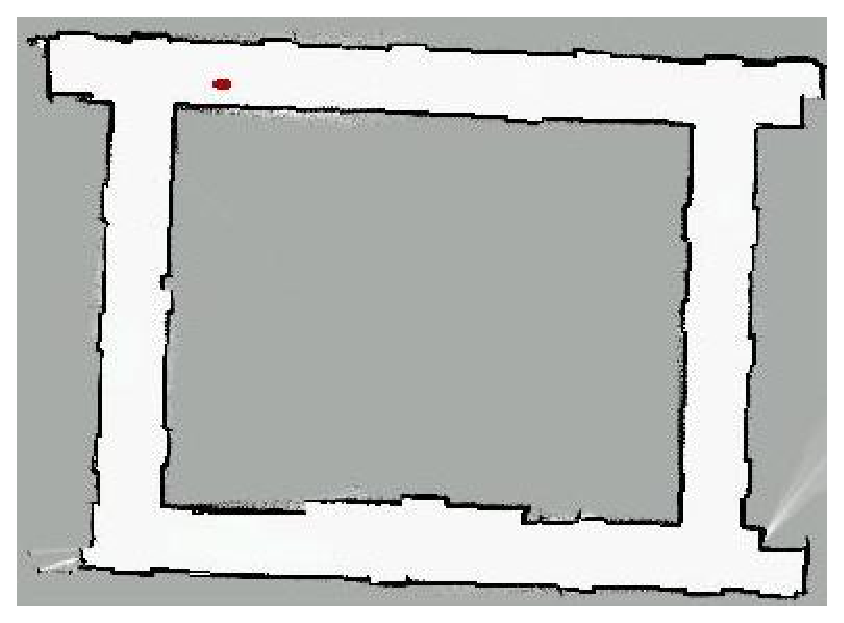
\epsfig{height=4cm,file=drivers/amcl-phe200-0800.eps} &
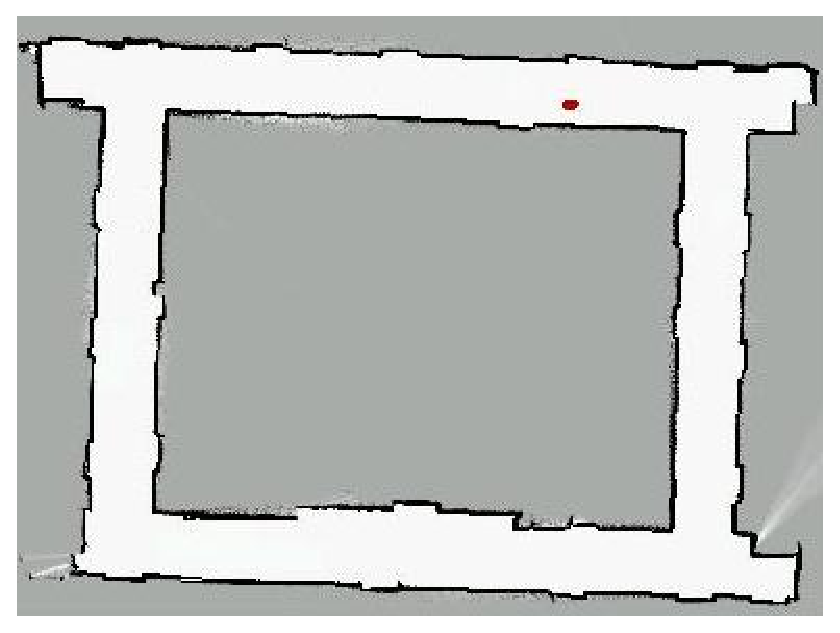
\epsfig{height=4cm,file=drivers/amcl-phe200-1200.eps} \\
$t = 80$~sec, $\approx 100$ particles & $t = 120$~sec, $\approx 100$ particles
\end{tabular}
\caption{Snap-shots showing the {\tt amcl} driver in action;
convergence in this case is relatively slow.}
\label{fig.amcl.example}
\end{center}
\end{figure*}


\subsection*{Caveats} 

At the time of writing, this driver is still evolving.  The sensor
models, in particular, are currently over-simplified and
under-parameterized (there are lots of magic numbers lurking about the
place).  Consequently, while this driver is known to work for certain
hardware configurations (think Pioneer2DX with a SICKLMS200 laser
range-finder), other configurations may require some refinement of the
sensor models.


\subsection*{Interfaces}

\noindent Supported interfaces:
\begin{itemize}
\item {\tt localize}
\end{itemize}

\noindent Required devices:
\begin{itemize}
\item {\tt position}
\item Any combination of: {\tt sonar}, {\tt laser} and {\tt wifi}.
\end{itemize}

\noindent Supported configuration requests:
\begin{itemize}
\item None.
\end{itemize}


\subsection*{Configuration file options}

\begin{center}
{\small \begin{tabularx}{\columnwidth}{|l|l|c|X|}
\hline
Name & Type & Default & Meaning\\
\hline

{\tt position\_index} & integer & 0 & Index of the position device to
use (this will usually be an odometric device of some sort). \\

{\tt sonar\_index} & integer & -1 & Index of the sonar ranging device
to use; set this to -1 if you dont wish to use sonar. \\

{\tt laser\_index} & integer & -1 & Index of the laser ranging device
to use; set this to -1 if you dont wish to use laser. \\

{\tt wifi\_index} & integer & -1 & Index of the WiFi signal-strength device
to use; set this to -1 if you dont wish to use WiFi signal-strength. \\

% Map options
{\tt map\_file} & filename & NULL & Name of the file containing the
occupancy map; see notes below for more on the map format. \\

{\tt map\_scale} & length & 0.05 & Scale of the map (meters/pixel). \\

{\tt map\_negate} & integer & 0 & Invert the states in the map
(occupied becomes empty and empty becomes occupied); see notes below. \\

% Odometic model
{\tt robot\_radius} & length & 0.20 & Effective radius of the robot
(meters); this value will be used to eliminate hypotheses that imply
that the robot is co-located with an obstacle. \\

% Sonar model

% Laser model
{\tt laser\_max\_samples} & integer & 5 & The maximum number of laser
range readings to use when updating the filter. \\

% WiFi model
{\tt wifi\_beacon\_N} & tuple & none & A tuple \verb+ [ "hostname"
"mapfilename" ]+ describing the $N^{\mathrm{th}}$ WiFi beacon.
{\tt hostname} specifies the name or IP address of the beacon; {\tt
mapfilename} points to the WiFi signal strength map for this
beacon. \\

% Particle filter
{\tt pf\_min\_samples} & integer & 100 & Lower bound on the number of
samples to maintain in the particle filter. \\

{\tt pf\_max\_samples} & integer & 10000 & Upper bound on the number of
samples to maintain in the particle filter. \\

{\tt pf\_err} & float & 0.01 & Control parameter for the particle set
size.  See notes below. \\

{\tt pf\_z} & float & 3 & Control parameter for the particle set
size.  See notes below. \\

% Initial conditions
{\tt init\_pose} & vector & [0 0 0] & Initial pose estimate (mean
value) for the robot (meters, meters, degrees). \\

{\tt init\_pose\_var} & vector & $[10^3 10^3 10^2]$ & Uncertainty in the
initial pose estimate (meters, meters, degrees). \\

% Debugging
{\tt enable\_gui} & integer & 0 & Set this to 1 to enable the built-in
driver GUI (useful for debugging).  Player must also be build with
{\tt configure --enable-rtkgui} for this option to have any effect. \\

\hline
\end{tabularx}}
\end{center}

\subsection*{Notes}

\begin{itemize}

\item {\bf Maps} 

The odometric, sonar and laser sensor models make use of a common
occupancy grid map.  This map is a regular grid in which cells are in
one of three states: occupied, empty or unknown (although the behavior
for unknown cells is currently undefined).  Maps are stored as
(uncompressed) images in PGM or PNM/grayscale format: black pixels are
treated as occupied cells, white pixels are treated as empty cells,
and the remaining colors are treated as unknown.  The interpretation
of these colors may be reversed (white is occupied, black is unknown)
by setting the {\tt map\_negate} flag in the configuration file.  This
flag is particularly handy if you wish to use the same image file as
both a map and a Stage bitmap.

TODO: WiFi maps

\item {\bf Coordinate System}

The origin of the global coordinate system corresponds to the center
of occupancy grid map.  Standard coordinate orientation is used; i.e.,
positive $x$ is towards the right of the map, positive $y$ towards the
top of the map.

\item {\bf Number of particles} 

The number of particles in the filter can be controlled using the
configuration file parameters {\tt pf\_err} and {\tt pf\_z}.
Specifically, {\tt pf\_err} is the maximum allowed error between the
true distribution and the estimated distribution, while {\tt pf\_z} is
the upper standard normal quantile for $(1 - p)$, where $p$ is the
probability that the error on the estimated distribution will be less
than {\tt pf\_err}.  If you dont know what that means, dont worry, I'm
not exactly sure either.  See \cite{fox01a} for a more meaningful
explanation.

\item {\bf Speed}

Many factors affect the speed at which the {\tt amcl} driver
runs, but the following tips might be helpful:
  \begin{itemize} 
  \item Reducing the number of laser range readings being used ({\tt
  laser\_max\_samples} in the configuration file) will significantly
  increase driver speed, but may also lead to slower convergence
  and/or less accurate localization.
  \item Increasing the allowed error {\tt pf\_err} and reducing the
  quantile {\tt pf\_z} will lead to smaller particle sets and will
  hence increase driver speed.  This may also lead, however, to
  over-convergence.
  \end{itemize}
As a benchmark, this driver has been successfully deployed on a
Pioneer2DX equipped with a SICK LMS200 and a 266MHz Mobile Pentium
with 32Mb of RAM.

\item {\bf Memory}

The two key factors affecting memory usage are:
  \begin{itemize}
  \item The size and resolution of the map.
  \item The maximum number of particles.
  \end{itemize}
As currently configured, the {\tt amcl} driver will typically use 10
to 20Mb of memory.  On embedded systems, where memory is at a premium,
users may have to decrease the map resolution or the maximum number of
particles to achieve acceptable preformance.


\end{itemize}




\subsection*{Example: Using the {\tt amcl} driver with a Pioneer robot}

The following configuration file illustrates the use of the {\tt
amcl} driver on a Pioneer robot equipped with a SICK LMS200
scanning laser range finder:
  \begin{small}
  \begin{verbatim}
  position:0 
  (
     driver "p2os_position" 
     port "/dev/ttyS1"
  )
  
  laser:0 
  (
    driver "sicklms200" 
    port "/dev/ttyS2"
  )

  localize:0 
  (
    driver "amcl"
    position_index 0
    laser_index 0
    map_file "mymap.pgm"
    map_scale 0.05
  )
  \end{verbatim}
  \end{small}
Naturally, the {\tt port}, {\tt map\_file} and {\tt map\_scale} values
should be changed to match your particular configuration.


\subsection*{Example: Using the {\tt amcl} driver with Stage}

The {\tt amcl} driver is not supported natively in Stage.
Users must therefore employ a second Player server configured to use
the {\tt passthrough} driver (see Section
\ref{sect:passthrough_driver}).  The basic procedure is as follows.
%
\begin{itemize}
\item Start Stage with a world file something like this:
  \begin{small}
  \begin{verbatim}
  ...
  position (port 6665 laser ())
  ...
  \end{verbatim}
  \end{small}
Stage will create one robot (position device) with a laser, and create
a Player server on port 6665.
\item Start another Player server using the command
  \begin{verbatim}
  player -p 7000 amcl.cfg
  \end{verbatim}
where the configuration file {\tt amcl.cfg} looks like this:
  \begin{small}
  \begin{verbatim}
  position:0 
  (
    driver "passthrough" 
    port 6665 index 0
  )

  laser:0 
  (
    driver "passthrough" 
    port 6665 
    index 0
  ) 

  localize:0 
  (
    driver "amcl" 
    position_index 0 
    laser_index 0 
    map_file "cave.pnm"
    map_scale 0.03
    map_negate 1
  )
  \end{verbatim}
  \end{small}
The second Player server will listen on port 7000; clients connecting
to this server will see a robot with {\tt position}, {\tt laser} and
{\tt localize} devices.  The map file {\tt cave.pnm} can be the same
file used by Stage to create the world bitmap.
\end{itemize}



\subsection*{Example: Using WiFi signal strength}

TODO




\newdriverex{amtecpowercube}{\gerkey}
\subsection*{Synopsis}
The {\tt amtecpowercube} driver provides control of an industrial-strength
pan-tilt unit called the PowerCube, made by Amtec.

\subsection*{Interfaces}

\noindent Supported interfaces:
\begin{itemize}
\item {\tt ptz}
\end{itemize}

\noindent Required devices:
\begin{itemize}
\item None.
\end{itemize}

\noindent Supported configuration requests:
\begin{itemize}
\item {\tt PLAYER\_PTZ\_CONTROL\_MODE\_REQ}
\end{itemize}

\subsection*{Configuration file options}

\begin{center}
{\small \begin{tabularx}{\columnwidth}{|l|l|c|X|}
\hline
Name & Type & Default & Meaning\\
\hline
{\tt port} & string & {\tt "/dev/ttyS0"} & The serial port to be used\\
{\tt home} & integer & {\tt 0} & Whether to home the unit before commanding it\\
{\tt speed} & integer & {\tt 40} & Maximum pan/tilt speed (deg/sec)\\
\hline
\end{tabularx}}
\end{center}

\subsection*{Notes}
\begin{itemize}
\item This driver is new and not thoroughly tested.
\item For constant swiveling, the PowerCube works better under velocity
control.
\end{itemize}


\newdriverex{cmucam2}{\pouya}
\subsection*{Synopsis}
The {\tt cmucam2} driver connects over a serial port to a
CMUCam2. Presents a blobfinder interface and can track multiple
color blobs. Provides data only; no commands or configs. This driver
is rudimentary but working. Color tracking parameters are defined in
Player's config file; for example:

\begin{verbatim}
  blobfinder(
    driver "cmucam2"
    devicepath "/dev/ttyS1"
    num_blobs 2
    # values must be between 40 and 240 (!)
    color0 [  red_min red_max blue_min blue_max green_min green_max] )
    # values must be between 40 and 240 (!)
    color1 [  red_min red_max blue_min blue_max green_min green_max] )  
  )
\end{verbatim}

\subsection*{Interfaces}

\noindent Supported interfaces:
\begin{itemize}
\item {\tt blobfinder}
\end{itemize}

\noindent Required devices:
\begin{itemize}
\item None.
\end{itemize}

\noindent Supported configuration requests:
\begin{itemize}
\item None.
\end{itemize}

\subsection*{Configuration file options}
{\bf TODO}

\subsection*{Notes}


\newdriverex{cmvision}{\andy,\gerkey,\brendan,\ben}

\subsection*{Synopsis}
CMVision (Color Machine Vision) is a fast color-segmentation (aka
blob-finding) software library.  CMVision was written by Jim Bruce at CMU
and is Freely available under the GNU GPL:\\
\indent {\tt http://www-2.cs.cmu.edu/$\sim$jbruce/cmvision/}\\
But you don't have to download CMVision yourself, because Player's 
{\tt cmvision} driver includes the CMVision code.  The {\tt cmvision}
driver provides a stream of camera images to the CMVision code and
assembles the resulting blob information into Player's {\tt blobfinder}
data format.

The frame-grabbing portion of the {\tt cmvision} driver is modular,
allowing the user to select the source of camera images.  Currently, the
following sources are supported (see below for how to select the capture
source).  Note that support for each source is compiled only if the
required libraries and/or kernel features are detected.
\begin{itemize}
\item IEEE 1394 (aka Firewire) cameras; requires the {\tt libraw1394} and
{\tt libdc1394} development packages (both are Freely available)
\item Video4Linux (aka V4L) cameras; requires V4L headers
\item Video4Linux2 (aka V4L2) cameras; requires V4L2 support in your
kernel ({\em currently disabled})
\item A video source that supports Player's internal {\tt camera}
interface, such as the Gazebo camera driver
\end{itemize}

\subsection*{Interfaces}

\noindent Supported interfaces:
\begin{itemize}
\item {\tt blobfinder}
\end{itemize}

\noindent Required devices:
\begin{itemize}
\item None.
\end{itemize}

\noindent Supported configuration requests:
\begin{itemize}
\item None.
\end{itemize}

\subsection*{Configuration file options}
\begin{center}
{\small \begin{tabularx}{\columnwidth}{|l|l|c|X|}
\hline
Name & Type & Default & Meaning\\
\hline
{\tt capture} & string & {\tt "1394"} & Capture source (should be {\tt
"1394"}, {\tt "V4L2"}, {\tt "V4L"}, or {\tt "camera"})\\
{\tt colorfile} & string & {\tt ""} & (absolute?) path to the CMVision configuration file.\\
{\tt height} & integer & {\tt 240} & Height of the camera images (pixels).\\
{\tt width} & integer & {\tt 320} & Width of the camera images (pixels).\\
\hline
\end{tabularx}}
\end{center}

\subsection*{Notes}
\begin{itemize}
\item This driver (or at least its underlying video capture code) only works in
Linux.
\item Consult the CMVision documentation for details on writing a CMVision
configuration file.
\end{itemize}



\newdriverexx{er1\_position}{er1_position}{\dfs}
\subsection*{Synopsis}
The {\tt er1} driver provides position control of the Evolution Robotics' ER1 and ERSDK robots.

\subsection*{Interfaces}

\noindent Supported interfaces:
\begin{itemize}
\item {\tt position}
\end{itemize}

\noindent Required devices:
\begin{itemize}
\item None.
\end{itemize}

\noindent Supported configuration requests:
\begin{itemize}
\item {\tt PLAYER\_POSITION\_GET\_GEOM\_REQ}
\item {\tt PLAYER\_POSITION\_MOTOR\_POWER\_REQ}
\end{itemize}

\subsection*{Configuration file options}

\begin{center}
{\small \begin{tabularx}{\columnwidth}{|l|l|c|X|}
\hline
Name & Type & Default & Meaning\\
\hline
{\tt port} & string & {\tt "/dev/usb/ttyUSB1"} & The serial port to be used\\
\hline
{\tt axle} & float & {\tt 0.38} & The distance between the motorized wheels\\
\hline
{\tt motor\_dir} & -1,1 & {\tt 1} & Direction of the motors, if the left motor is plugged in to the motor 1 port on the RCM, put -1 here instead\\
\hline
{\tt debug} & 0,1 & {\tt 0} & Put a 1 here if you want to see debug messages\\
\hline
\end{tabularx}}
\end{center}


\subsection*{Notes}
\begin{itemize}
\item This driver is new and not thoroughly tested.  The odometry cannot be trusted to give accurate readings.

\item You will need a kernel driver to allow the serial port to be seen.  This driver, and news about the player driver can be found at "http://www-robotics.usc.edu/~dfseifer/project-erplayer.php".

\item TODO: split this driver similar to the way that p2os is split, one main body device, and sub-devices like position, and IR which inherit from this main class.  Implement power interface.

\item NOT DOING: I don't have a gripper, if someone has code for a gripper, by all means contribute it.  It would be welcome to the mix.
\end{itemize}


\newdriverex{festival}{\gerkey}
\subsection*{Synopsis}
The {\tt festival} driver provides access to the Festival speech synthesis
system.  Festival is available separately (also under the GNU GPL) at:
\verb+http://www.cstr.ed.ac.uk/projects/festival/+.  Unlike most drivers, the
{\tt festival} driver queues incoming commands, rather than overwriting them.
When the queue is full, new commands are discarded.

\subsection*{Interfaces}

\noindent Supported interfaces:

\begin{itemize}
\item {\tt speech}
\end{itemize}

\noindent Required devices:
\begin{itemize}
\item None.
\end{itemize}

\noindent Supported configuration requests:
\begin{itemize}
\item None.
\end{itemize}


\subsection*{Configuration file options}

\begin{center}
{\small \begin{tabularx}{\columnwidth}{|l|l|c|X|}
\hline
Name & Type & Default & Meaning\\
\hline
{\tt port} & integer & {\tt 1314} & The TCP port on which Player should
communicate with Festival.\\
{\tt libdir} & string & {\tt "/usr/local/festival/lib"} & Festival's library
directory.\\
{\tt queuelen} & integer & {\tt 4} & The length of the incoming command
queue.\\
\hline
\end{tabularx}}
\end{center}

\subsection*{Notes}


\newdriverex{fixedtones}{\esben,\gerkey}
\subsection*{Synopsis}
The {\tt fixedtones} driver provides access to sound hardware, via the Linux
OSS interface.  Incoming sound is put through a Discrete Fourier Transform,
and the frequencies and amplitudes of the five highest peaks in the frequency
domain are determined.  Note that the {\tt FFTW} library is required; this
package is available (also under the GNU GPL) from: {\tt http://www.fftw.org}.
The {\tt fixedtones} driver can also produce fixed-tone sounds of given
frequency, amplitude, and duration.


\subsection*{Interfaces}

\noindent Supported interfaces:
\begin{itemize}
\item {\tt audio}
\end{itemize}

\noindent Required devices:
\begin{itemize}
\item None.
\end{itemize}

\noindent Supported configuration requests:
\begin{itemize}
\item None.
\end{itemize}


\subsection*{Configuration file options}
No configuration file options are supported.

\subsection*{Notes}
\begin{itemize}
\item This driver is not widely used and may not function properly.
\end{itemize}


\newdriverex{flockofbirds}{\toby}
\subsection*{Synopsis}
The {\tt flockofbirds} driver provides a basic interface to the ascension
Flock of Birds 6DOF position tracker.

This driver ignores all commands and configuration requests and simple provides a 
continuous stream of position updates from a single flock of birds controller.

There is currently no support for multiple trackers.

\subsection*{Interfaces}

\noindent Supported interfaces:

\begin{itemize}
\item {\tt position3d}
\end{itemize}

\noindent Supported configuration requests:
\begin{itemize}
\item None.
\end{itemize}


\subsection*{Configuration file options}
\begin{itemize}
\item None.
\end{itemize}


\newdriverex{garminnmea}{\gerkey,\ahoward}
\subsection*{Synopsis}

The {\tt garminnmea} driver controls a Garmin handheld GPS unit, via a
RS232 link.  The driver was developed using the Garmin Geko 201, but
it should work with other Garmin units.  It is unlikely to work with
non-Garmin GPS units, as at least one proprietary Garmin NMEA
sentences is being used.

This driver is also capable of operating the unit in DGPS mode using
RTCM corrections.  The driver listens on a network socket for RTCM
packets generated by a remote DGPS base station; the packets are
forwarded over the serial port to the GPS unit, which responds by
switching into DGPS mode.  The {\tt dgps\_server} utility found in the
{\tt utils/dgps\_server} directory may be used to generate RTCM
corrections; corrections are transmitted to clients using UDP
multicast.


\subsection*{Interfaces}

\noindent Supported interfaces:
\begin{itemize}
\item {\tt gps}
\end{itemize}

\noindent Required devices:
\begin{itemize}
\item None.
\end{itemize}

\noindent Supported configuration requests:
\begin{itemize}
\item None.
\end{itemize}

\subsection*{Configuration file options}

\begin{center}
{\small \begin{tabularx}{\columnwidth}{|l|l|c|X|}
\hline
Name & Type & Default & Meaning\\
\hline
{\tt port} & string & {\tt "/dev/ttyS0"} & The serial port to be used\\
{\tt dgps\_enable} & integer & 1 & Enable DGPS RTCM forwarding \\
{\tt dgps\_group} & string & {\tt 225.0.0.43} & Multicast group for RTCM corrections \\
{\tt dgps\_port} & integer & 7778 & Port number for RTCM corrections \\
\hline
\end{tabularx}}
\end{center}

\subsection*{Notes}




\newdriverexx{gz\_camera}{gz_camera}{\ahoward}
\subsection*{Synopsis}

The {\tt gz\_camera} driver is used to access Gazebo models that
support the camera interface (such as the SonyVID model).

\subsection*{Interfaces}

\noindent Supported interfaces:
\begin{itemize}
\item {\tt camera}
\end{itemize}

\noindent Required devices:
\begin{itemize}
\item None.
\end{itemize}

%\noindent Supported configuration requests:
%\begin{itemize}
%\end{itemize}


\subsection*{Configuration file options}

\begin{center}
{\small \begin{tabularx}{\columnwidth}{|l|l|c|X|}
\hline
Name & Type & Default & Meaning\\
\hline
{\tt gz\_id} & string & {\tt NULL} & ID of the Gazebo model. \\
\hline
\end{tabularx}}
\end{center}

\subsection*{Notes}

Consult the Gazebo manual for more information on the Gazebo
simulation package.



\newdriverexx{gz\_gripper}{gz_gripper}{\ahoward}
\subsection*{Synopsis}

The {\tt gz\_gripper} driver is used to access Gazebo models that
support the gripper interface (such as the SonyVID model).

\subsection*{Interfaces}

\noindent Supported interfaces:
\begin{itemize}
\item {\tt gripper}
\end{itemize}

\noindent Required devices:
\begin{itemize}
\item None.
\end{itemize}

%\noindent Supported configuration requests:
%\begin{itemize}
%\end{itemize}


\subsection*{Configuration file options}

\begin{center}
{\small \begin{tabularx}{\columnwidth}{|l|l|c|X|}
\hline
Name & Type & Default & Meaning\\
\hline
{\tt gz\_id} & string & {\tt NULL} & ID of the Gazebo model. \\
\hline
\end{tabularx}}
\end{center}

\subsection*{Notes}

Consult the Gazebo manual for more information on the Gazebo
simulation package.



\newdriverexx{gz\_laser}{gz_laser}{\ahoward}
\subsection*{Synopsis}

The {\tt gz\_laser} driver is used to access Gazebo models that
support the laser interface (such as the SickLMS200 model).

\subsection*{Interfaces}

\noindent Supported interfaces:
\begin{itemize}
\item {\tt laser}
\end{itemize}

\noindent Required devices:
\begin{itemize}
\item None.
\end{itemize}

\noindent Supported configuration requests:
\begin{itemize}
\item \verb+PLAYER_LASER_GET_GEOM+
\end{itemize}


\subsection*{Configuration file options}

\begin{center}
{\small \begin{tabularx}{\columnwidth}{|l|l|c|X|}
\hline
Name & Type & Default & Meaning\\
\hline
{\tt gz\_id} & string & {\tt NULL} & ID of the Gazebo model. \\
\hline
\end{tabularx}}
\end{center}

\subsection*{Notes}

Consult the Gazebo manual for more information on the Gazebo
simulation package.



\newdriverexx{gz\_position}{gz_position}{\ahoward}
\subsection*{Synopsis}

The {\tt gz\_postion} driver is used to access Gazebo models that
support the position interface (generally speaking, these are robots
such as the Pioneer2AT).  

\subsection*{Interfaces}

\noindent Supported interfaces:
\begin{itemize}
\item {\tt position}
\end{itemize}

\noindent Required devices:
\begin{itemize}
\item None.
\end{itemize}

%\noindent Supported configuration requests:
%\begin{itemize}
%\item \verb+PLAYER_POSITION_GET_GEOM+
%\end{itemize}


\subsection*{Configuration file options}

\begin{center}
{\small \begin{tabularx}{\columnwidth}{|l|l|c|X|}
\hline
Name & Type & Default & Meaning\\
\hline
{\tt gz\_id} & string & {\tt NULL} & ID of the Gazebo model. \\
\hline
\end{tabularx}}
\end{center}

\subsection*{Notes}

Consult the Gazebo manual for more information on the Gazebo
simulation package.



\newdriverexx{gz\_position3d}{gz_position3d}{\ahoward}
\subsection*{Synopsis}

The {\tt gz\_postion3d} driver is used to access Gazebo models that
support the position interface (generally speaking, these are robots
such as the Pioneer2AT).  

\subsection*{Interfaces}

\noindent Supported interfaces:
\begin{itemize}
\item {\tt position3d}
\end{itemize}

\noindent Required devices:
\begin{itemize}
\item None.
\end{itemize}

%\noindent Supported configuration requests:
%\begin{itemize}
%\end{itemize}


\subsection*{Configuration file options}

\begin{center}
{\small \begin{tabularx}{\columnwidth}{|l|l|c|X|}
\hline
Name & Type & Default & Meaning\\
\hline
{\tt gz\_id} & string & {\tt NULL} & ID of the Gazebo model. \\
\hline
\end{tabularx}}
\end{center}

\subsection*{Notes}

Consult the Gazebo manual for more information on the Gazebo
simulation package.



\newdriverexx{gz\_power}{gz_power}{\ahoward}
\subsection*{Synopsis}

The {\tt gz\_power} driver is used to access Gazebo models that
support the power interface.

\subsection*{Interfaces}

\noindent Supported interfaces:
\begin{itemize}
\item {\tt power}
\end{itemize}

\noindent Required devices:
\begin{itemize}
\item None.
\end{itemize}

%\noindent Supported configuration requests:
%\begin{itemize}
%\end{itemize}


\subsection*{Configuration file options}

\begin{center}
{\small \begin{tabularx}{\columnwidth}{|l|l|c|X|}
\hline
Name & Type & Default & Meaning\\
\hline
{\tt gz\_id} & string & {\tt NULL} & ID of the Gazebo model. \\
\hline
\end{tabularx}}
\end{center}

\subsection*{Notes}

Consult the Gazebo manual for more information on the Gazebo
simulation package.



\newdriverexx{gz\_ptz}{gz_ptz}{\ahoward}
\subsection*{Synopsis}

The {\tt gz\_ptz} driver is used to access Gazebo models that
support the ptz interface.

\subsection*{Interfaces}

\noindent Supported interfaces:
\begin{itemize}
\item {\tt ptz}
\end{itemize}

\noindent Required devices:
\begin{itemize}
\item None.
\end{itemize}

%\noindent Supported configuration requests:
%\begin{itemize}
%\end{itemize}


\subsection*{Configuration file options}

\begin{center}
{\small \begin{tabularx}{\columnwidth}{|l|l|c|X|}
\hline
Name & Type & Default & Meaning\\
\hline
{\tt gz\_id} & string & {\tt NULL} & ID of the Gazebo model. \\
\hline
\end{tabularx}}
\end{center}

\subsection*{Notes}

Consult the Gazebo manual for more information on the Gazebo
simulation package.



\newdriverexx{gz\_sonar}{gz_sonar}{\ahoward}
\subsection*{Synopsis}

The {\tt gz\_sonar} driver is used to access Gazebo models that
support the sonars interface.

\subsection*{Interfaces}

\noindent Supported interfaces:
\begin{itemize}
\item {\tt sonar}
\end{itemize}

\noindent Required devices:
\begin{itemize}
\item None.
\end{itemize}

%\noindent Supported configuration requests:
%\begin{itemize}
%\end{itemize}


\subsection*{Configuration file options}

\begin{center}
{\small \begin{tabularx}{\columnwidth}{|l|l|c|X|}
\hline
Name & Type & Default & Meaning\\
\hline
{\tt gz\_id} & string & {\tt NULL} & ID of the Gazebo model. \\
\hline
\end{tabularx}}
\end{center}

\subsection*{Notes}

Consult the Gazebo manual for more information on the Gazebo
simulation package.



\newdriverexx{gz\_truth}{gz_truth}{\ahoward}
\subsection*{Synopsis}

The {\tt gz\_truth} driver is used to access Gazebo models that
support the truth interface.

\subsection*{Interfaces}

\noindent Supported interfaces:
\begin{itemize}
\item {\tt truth}
\end{itemize}

\noindent Required devices:
\begin{itemize}
\item None.
\end{itemize}

%\noindent Supported configuration requests:
%\begin{itemize}
%\end{itemize}


\subsection*{Configuration file options}

\begin{center}
{\small \begin{tabularx}{\columnwidth}{|l|l|c|X|}
\hline
Name & Type & Default & Meaning\\
\hline
{\tt gz\_id} & string & {\tt NULL} & ID of the Gazebo model. \\
\hline
\end{tabularx}}
\end{center}

\subsection*{Notes}

Consult the Gazebo manual for more information on the Gazebo
simulation package.




\newdriverex{khepera}{\toby}
\subsection*{Synopsis}
The {\tt khepera\_*} family of drivers are used to interface to the K-Team khepera robot. 

This driver is experimental and should be treated with caution. At this point it supports the position and ir interfaces.

\subsection*{Interfaces / Configuration requests}
Like the P2OS device, one thread handles 2 separate devices: position and IR. 
\begin{itemize}
	\item \texttt{khepera\_position}
	\begin{itemize}
		\item Interface: {\tt position} (see Section~\ref{sect:position})
		\item Configurations: {\tt GET\_GEOM}, {\tt MOTOR\_POWER}, 
			{\tt VELOCITY\_MODE}, {\tt RESET\_ODOM}
		\end{itemize}
	
	\item {\tt khepera\_ir}
	
	\begin{itemize}
		\item Interface: {\tt ir} (see Section~\ref{sect:ir})
		\item Configurations: {\tt POSE}
	\end{itemize}

\end{itemize}
\subsection*{Configuration file options}
Table~\ref{table:khepera_options} lists the available configuration file options for the Khepera device.  If an option is specified more than once in the config file, then only the first value will be used.

\begin{table}[ht]
\begin{center}
{\small \begin{tabular}{|l|l|c|l|l|l|} \hline
Name & Type & Default & Supported by &  Values & Meaning \\ \hline
{\tt port} & string & {\tt /dev/ttyUSB0} & {\tt khepera\_*} &  & This port connects to the Khepera.\\ \hline
{\tt scale} & float & {\tt 10} & {\tt khepera\_*} & & As the khepera is so small the actual geometry doesnt make much sense with many of the existing defaults so the geometries can all be scaled by this factor. \\ \hline

{\tt encoder\_res} & float & {\tt 1/12} & {\tt khepera\_position } & & The wheel encoder resolution. \\ \hline
{\tt pose} & float tuple & {\tt [0 0 0]} & {\tt khepera\_position } & & The pose of the robot in player coordinates (mm, mm, deg). \\ \hline
{\tt size} & float tuple & {\tt [57 57]} & {\tt khepera\_position } & & The size of the robot approximated to a rectangle (mm, mm). \\ \hline

{\tt pose\_count} & int & {\tt 8} & {\tt khepera\_ir } & & The number of ir poses. \\ \hline
{\tt poses} & float tuple & {\tt Khepera poses} & {\tt khepera\_ir } & & The pose of each ir sensor [mm,mm,deg] \\ \hline

\end{tabular}}
\end{center}
\caption{{\em Configuration file options for the {\tt khepera\_*} drivers}.}
\label{table:khepera_options}
\end{table}



\newdriverex{lasercspace}{\ahoward}

\begin{figure}[ht]
\begin{center}
\begin{tabular}{cc}
\frame{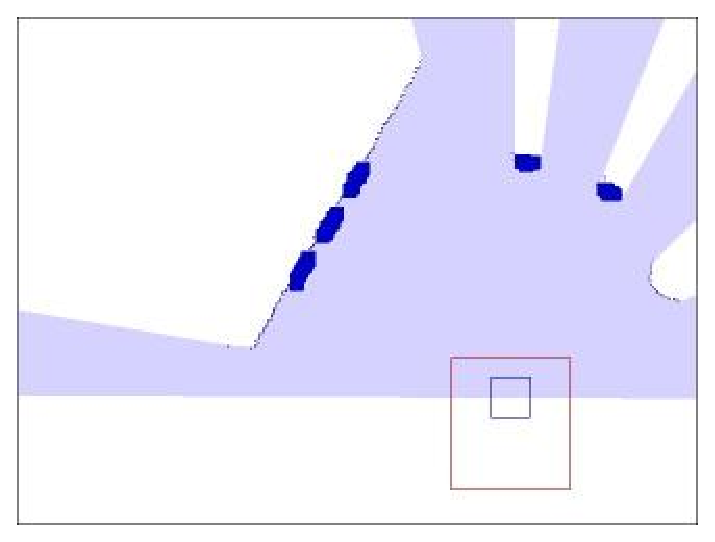
\epsfig{file=drivers/lasercspace-1.eps, height=40mm}} &
\frame{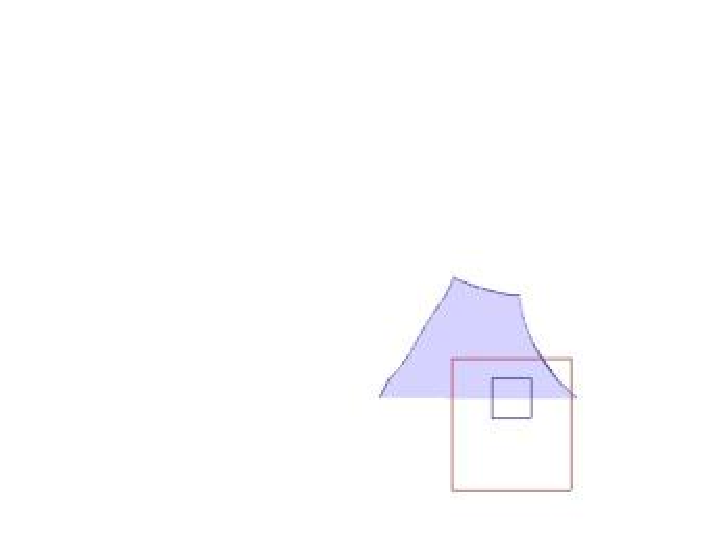
\epsfig{file=drivers/lasercspace-2.eps, height=40mm}} \\
(a) & (b) \\
\end{tabular}
\caption{(a) Standard laser scan.  (b) The corresponding C-space scan 
for a robot of radius 0.05~m}
\label{fig:lasercspace}
\end{center}
\end{figure}

\subsection*{Synopsis}

The lasercspace driver processes a laser scan to compute the
configuration space (`C-space') boundary.  That is, it shortens the
range of each laser scan such that the resultant scan delimits the
obstacle-free portion of the robot's configuration space.  This driver
is particular useful for writing obstacle avoidance algorithms, since the
robot may safely move to any point in the obstacle-free portion of the 
configuration space.

Note that driver computes the configuration space for a robot of some
fixed radius; this radius may be set in the configuration file.


\subsection*{Interfaces}

\noindent Supported interfaces:
\begin{itemize}
\item {\tt laser}
\end{itemize}

\noindent Required devices:
\begin{itemize}
\item {\tt laser}
\end{itemize}

\noindent Supported configuration requests:
\begin{itemize}
\item \verb+PLAYER_LASER_GET_GEOM+
\end{itemize}

\subsection*{Configuration file options}

\begin{center}
{\small \begin{tabularx}{\columnwidth}{|l|l|c|X|}
\hline
Name & Type & Default & Meaning\\
\hline
\verb+laser+ & integer & 0 & Index of the laser device to use. \\
\verb+radius+ & length & 0.50 & Robot radius. \\
\hline
\end{tabularx}}
\end{center}


\subsection*{Notes}


\newdriverex{laserbar}{\ahoward}

\begin{figure}[ht]
\begin{center}
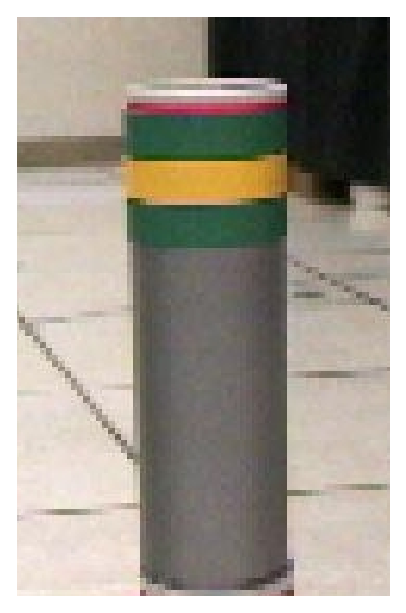
\epsfig{file=laservisualbeacon.eps, height=40mm}
\caption{A sample laser bar (ignore the colored bands).}
\label{fig:laserbar}
\end{center}
\end{figure}

\subsection*{Synopsis}

The laser bar detector searches for retro-reflective targets in the
laser range finder data.  Targets can be either planar or cylindrical,
as shown in Figure \ref{fig:laserbar}.  For planar targets, the range,
bearing and orientation will be determined; for cylindrical targets,
only the range and bearing will be determined.  The target size and
shape can be set in the configuration file.

The range at which targets can be detected is dependant on the target
size, the angular resolution of the laser and the quality of the
retro-reflective material used on the target.

See also the {\tt laserbarcode} and {\tt laservisualbarcode} drivers.

\subsection*{Interfaces}

\noindent Supported interfaces:
\begin{itemize}
\item {\tt fiducial}
\end{itemize}

\noindent Required devices:
\begin{itemize}
\item {\tt laser}
\end{itemize}

\noindent Supported configuration requests:
\begin{itemize}
\item \verb+PLAYER_FIDUCIAL_GET_GEOM+
\end{itemize}


\subsection*{Configuration file options}

\begin{center}
{\small \begin{tabularx}{\columnwidth}{|l|l|c|X|}
\hline
Name & Type & Default & Meaning\\
\hline
{\tt laser} & integer & 0 & Index of the {\tt laser} device to be used. \\
{\tt shape} & string & ``cylinder'' & Target shape: ``plane'' or ``cylinder''. 
Planar fiducials are currently not supported.\\
{\tt width} & length & 0.08 & Target width (m). \\
\hline
\end{tabularx}}
\end{center}

\subsection*{Notes}


\newdriverex{laserbarcode}{\ahoward}

\begin{figure}[ht]
\begin{center}
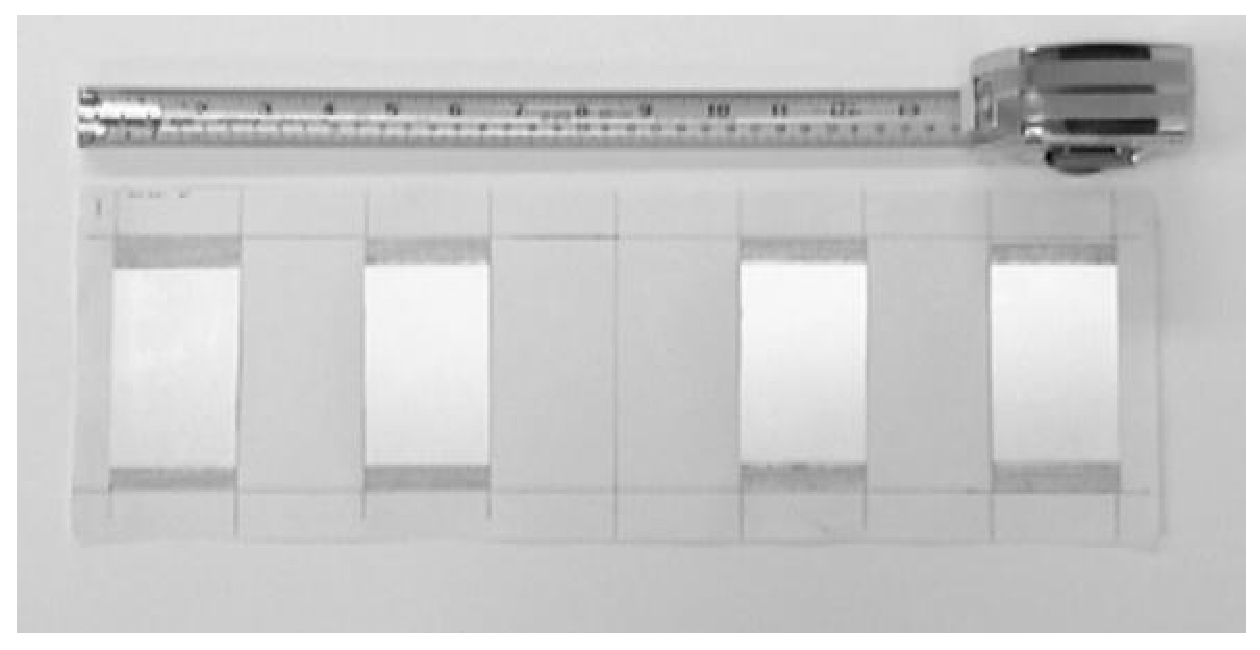
\epsfig{file=beacon.eps, height=40mm}
\caption{A sample laser barcode.  This barcode has 8 bits, each of which 
is 50mm wide.}
\label{fig:laserbarcode}
\end{center}
\end{figure}

\subsection*{Synopsis}

The laser barcode detector searches for specially constructed barcodes
in the laser range finder data.  An example laser barcode is shown in
Figure \ref{fig:laserbarcode}.  The barcode is constructed using
strips of retro-reflective paper.  Each retro-reflective strip
represents a `1' bit; each non-reflective strip represents a `0' bit.
By default, the {\tt laserbarcode} driver searches for barcodes
containing 8 bits, each of which is exactly 50mm wide (the total
barcode width is thus 400m).  The first and last bits are used as
start and end markers, and the remaining bits are used to determine
the identity of the barcode; with an 8-bit barcode there are 64 unique
IDs.  The number of bits and the width of each bit can be set in the
configuration file.

The range at which barcodes can be detected {\em and identified} is dependent
on the bit width and the angular resolution of the laser.  With 50mm bits and
an angular resolution of $0.5^\circ$, barcodes can be detected and identified
at a range of about 2.5m.  With the laser resolution set to  $0.25^\circ$,
this distance is roughly doubled to about 5m.

See also the {\tt laserbar} and {\tt laservisualbarcode} drivers.


\subsection*{Interfaces}

\noindent Supported interfaces:
\begin{itemize}
\item {\tt fiducial}
\end{itemize}

\noindent Required devices:
\begin{itemize}
\item {\tt laser}
\end{itemize}

\noindent Supported configuration requests:
\begin{itemize}
\item \verb+PLAYER_FIDUCIAL_GET_GEOM+
\end{itemize}



\subsection*{Configuration file options}

\begin{center}
{\small \begin{tabularx}{\columnwidth}{|l|l|c|X|}
\hline
Name & Type & Default & Meaning\\
\hline
{\tt laser} & integer & 0 & Index of the {\tt laser} device to be used.\\
{\tt bit\_count} & integer & {\tt 8} & The number of bits in the barcodes.\\
{\tt bit\_width} & length & {\tt 0.05} & The width of each bit in the barcode
(m).\\
\hline
\end{tabularx}}
\end{center}

\subsection*{Notes}

For more information on the {\tt laserbarcode} driver, ask Andrew Howard:
{\tt ahoward@usc.edu}.


\newdriverex{laservisualbarcode}{\ahoward}


\begin{figure}[ht]
\begin{center}
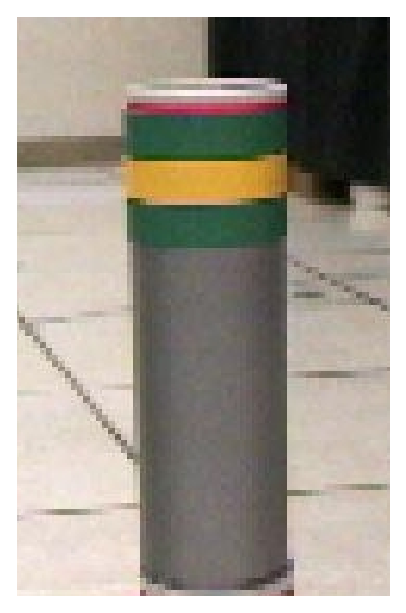
\epsfig{file=laservisualbeacon.eps, height=40mm}
\caption{A sample laser visual barcode.}
\label{fig:laservisualbarcode}
\end{center}
\end{figure}

\subsection*{Synopsis}

The laser visual barcode detector uses both searches for fiducials
that are both retro-reflective and color-coded.  Fiducials can be
either planar or cylindical, as shown in Figure
\ref{fig:laservisualbarcode}.  For planar targets, the range, bearing,
orientation and identity will be determined; for cylindrical targets,
the orientation will be undefined.  The target size and shape can be
set in the configuration file.

The laser visual barcode detector searches the laser range data to
find retro-reflective targets, points the camera at each of these
targets in turn, then uses color information to determine the presence
and identity of fiducials.  Thus, this detector makes use of three
underlying devices: a laser range finder, a pan-tilt-zoom camera and a
color blob detector.  Note that the laser is used to determine the
geometry of the fidicual (range, bearing and orientation), while the
camera is used to determine its identity.

The range at which fiducials can be both detected and identified
depends on a number of factors, including the size of the fiducial and
the angular resolution of the laser.  Generally speaking, however,
this detector has better range than the {\tt laserbarcode} detector,
but produces fewer observations.

See also the {\tt laserbar} and {\tt laserbarcode} drivers.


\subsection*{Interfaces}

\noindent Supported interfaces:
\begin{itemize}
\item {\tt fiducial}
\end{itemize}

\noindent Required devices:
\begin{itemize}
\item {\tt laser}
\item {\tt ptz}
\item {\tt blobfinder}
\end{itemize}

\noindent Supported configuration requests:
\begin{itemize}
\item \verb+PLAYER_FIDUCIAL_GET_GEOM+
\end{itemize}


\subsection*{Configuration file options}

\begin{center}
{\small \begin{tabularx}{\columnwidth}{|l|l|c|X|}
\hline
Name & Type & Default & Meaning\\
\hline
{\tt laser} & integer & 0 & Index of the {\tt laser} device to be used.\\
{\tt ptz} & integer & 0 & Index of the {\tt ptz} device to be used.\\
{\tt blobfinder} & integer & 0 & Index of the {\tt blobfinder} device to be used.\\
{\tt shape} & string & ``cylinder'' & Target shape: ``plane'' or ``cylinder''.
Planar fiducials are currently not supported. \\
{\tt bit\_count} & integer & {\tt 8} & The number of bits in the barcode.\\
{\tt bit\_width} & length & {\tt 0.05} & The width of each bit in the barcode (m).\\
{\tt bit\_height} & length & {\tt 0.05} & The height of each bit in the barcode (m).\\
\hline
\end{tabularx}}
\end{center}

\subsection*{Notes}

Setting up the laser-visual barcode detector can be a bit tricky,
since it involves so many underlying devices.  Users should first
check that the {\tt laser}, {\tt ptz} and {\tt blobfinder} devices are
working before attempting to use the {\tt laservisualbarcode} driver.
Note that the {\tt blobfinder} device must be calibrated to detect the
particular colors used in the fiducials, and that the identity
assigned to each fiducial is determined by the color-to-channel
mapping chosen during this configuration.

For more information on the {\tt laserbarcode} driver, ask Andrew Howard:
{\tt ahoward@usc.edu}.


\newdriverex{lifo-mcom}{\brewer,\reed}

\subsection*{Synopsis}
 The {\tt lifo\_mcom} driver provides a last-in-first-out (LIFO)
 multi-stack communication system with which clients can exchange data
 through an instance of Player.

 If Pop is called, the last piece of data that was Pushed to the named
 channel is returned and then deleted.  If Read is called the last piece
 of data added is returned, and left there.  Since this is a LIFO stack,
 if we're reading drive commands, for example, we can be sure to get a
 "STOP" and interrupt a "FWD" before it's been read.

\subsection*{Interfaces}

\noindent Supported interfaces:
\begin{itemize}
\item {\tt mcom}
\end{itemize}

\noindent Required devices:
\begin{itemize}
\item None.
\end{itemize}

\noindent Supported configuration requests:
\begin{itemize}
\item None.
\end{itemize}

\subsection*{Configuration file options}
No configuration file options are supported.



\newdriverex{linuxwifi}{\sweeney}
\subsection*{Synopsis}
The {\tt linux\_wifi} driver provides access to information about
wireless Ethernet cards in Linux.


\subsection*{Interfaces}

\noindent Supported interfaces:

\begin{itemize}
\item {\tt wifi}
\end{itemize}

\noindent Required devices:
\begin{itemize}
\item None.
\end{itemize}

\noindent Supported configuration requests:
\begin{itemize}
\item None.
\end{itemize}


\subsection*{Configuration file options}
No configuration file options are accepted.

\subsection*{Notes}
This driver simply parses the contents of {\tt /proc/net/wireless}.


\newdriverex{mixer}{\nate}
% mixer

\subsection*{Synopsis}

TODO


\subsection*{Interfaces}

\noindent Supported interfaces:

\begin{itemize}
\item {\tt audiomixer}
\end{itemize}

\noindent Required devices:
\begin{itemize}
\item None.
\end{itemize}

\noindent Supported configuration requests:
\begin{itemize}
\item TODO
\end{itemize}


\subsection*{Configuration file options}

TODO

\subsection*{Notes}

TODO


\newdriverex{nomad}{\vaughan,\pawel}
\subsection*{Synopsis}
The {\tt nomad} driver connects over a serial port to a Nomad 200
robot running Nomadics' ``robotd'' daemon.   Data and commands are handled
via the custom {\tt nomad} interface.

The {\tt nomad\_position} and {\tt nomad\_sonar} drivers provide data in
the standard position and sonar interfaces.  Position interface provides
data, takes commands and supports geometry config.  Sonar interface
provides data and supports geometry config. This driver is rudimentary
but tested and working on the Nomad 200. It may also work on other Nomads
that run robotd.

\subsection*{Interfaces}

\noindent Supported interfaces:
\begin{itemize}
\item {\tt nomad}
\item {\tt position}
\item {\tt sonar}
\end{itemize}

\noindent Required devices:
\begin{itemize}
\item None.
\end{itemize}

\noindent Supported configuration requests:
\begin{itemize}
\item {\tt GET\_GEOM} (position and sonar)
\end{itemize}

\subsection*{Configuration file options}

\noindent {\tt nomad}:\\
\begin{center}
{\small \begin{tabularx}{\columnwidth}{|l|l|c|X|}
\hline
Name & Type & Default & Meaning\\
\hline
{\tt serial\_device} & string & {\tt ""} & The serial port to be used\\
{\tt serial\_speed} & int & {\tt -1} & The baud rate to use \\
\hline
\end{tabularx}}
\end{center}

\noindent {\tt nomad\_position}:\\
\begin{center}
{\small \begin{tabularx}{\columnwidth}{|l|l|c|X|}
\hline
Name & Type & Default & Meaning\\
\hline
{\tt nomad\_index} & int & {\tt 0} & The index of the underlying nomad
device.\\
\hline
\end{tabularx}}
\end{center}

\noindent {\tt nomad\_sonar}:\\
\begin{center}
{\small \begin{tabularx}{\columnwidth}{|l|l|c|X|}
\hline
Name & Type & Default & Meaning\\
\hline
{\tt nomad\_index} & int & {\tt 0} & The index of the underlying nomad
device.\\
\hline
\end{tabularx}}
\end{center}

\subsection*{Notes}


\newdriverex{p2os}{\gerkey,\kasper,\mckenna}
\subsection*{Synopsis}
Many robots made by ActivMedia, such as the Pioneer series and the AmigoBot,
are controlled by a microcontroller that runs a special embedded operating
system called P2OS (on older robots it is called PSOS).  The host computer
talks to the P2OS microcontroller over a standard RS232 serial line.  Player
includes a driver that offer access to the various P2OS-mediated devices,
logically splitting up the devices' functionality.

\subsection*{Interfaces / Configuration requests}
Although all the P2OS interaction is actually done in a single thread, the
different P2OS devices are accessed through different Player drivers, each
supporting a different interface and supporting some subset of configuration
requests:
\begin{itemize}
\item {\tt p2os\_aio}:
  \begin{itemize}
  \item Interface: {\tt aio} (see Section~\ref{sect:aio})
  \item Configurations: none
  \item Notes: Provides access to analog User I/O.
  \end{itemize}
\item {\tt p2os\_bumper}:
  \begin{itemize}
  \item Interface: {\tt bumper} (see Section~\ref{sect:bumper})
  \item Configurations: none
  \item Notes: Provides access to Pioneer bumpers, for those robots so equipped.
  \end{itemize}
\item {\tt p2os\_cmucam}:
  \begin{itemize}
  \item Interface: {\tt blobfinder} (see Section~\ref{sect:blobfinder})
  \item Configurations: {\tt SET\_COLOR}, {\tt SET\_IMAGER\_PARAMS}
  \item Notes: Controls a CMUCam that is connected to the AUX2 port on the
               P2OS board.  Use the {\tt SET\_COLOR} request to tell the
               camera which color to track.
  \end{itemize}
\item {\tt p2os\_compass}:
  \begin{itemize}
  \item Interface: {\tt position} (see Section~\ref{sect:position})
  \item Configurations: none
  \item Notes: Fills the compass heading into the {\tt yaw} field of the {\tt
  position} data packet.  Accepts no commands.
  \end{itemize}
\item {\tt p2os\_dio}:
  \begin{itemize}
  \item Interface: {\tt dio} (see Section~\ref{sect:dio})
  \item Configurations: none
  \item Notes: Provides access to digital User I/O.
  \end{itemize}
\item {\tt p2os\_gripper}:
  \begin{itemize}
  \item Interface: {\tt gripper} (see Section~\ref{sect:gripper})
  \item Configurations: none
  \item Notes: Provides access to a Pioneer gripper, for those robots so
        equipped.
  \end{itemize}
\item {\tt p2os\_position}:
  \begin{itemize}
  \item Interface: {\tt position} (see Section~\ref{sect:position})
  \item Configurations: {\tt GET\_GEOM}, {\tt MOTOR\_POWER}, {\tt
  VELOCITY\_MODE}, {\tt RESET\_ODOM}
  \item Notes: Provides access to a differential wheelbase.  Only speed control 
  is supported.
  \end{itemize}
\item {\tt p2os\_power}:
  \begin{itemize}
  \item Interface: {\tt power} (see Section~\ref{sect:power})
  \item Configurations: none
  \item Notes: Provides access to battery charge information.
  \end{itemize}
\item {\tt p2os\_sonar}:
  \begin{itemize}
  \item Interface: {\tt sonar} (see Section~\ref{sect:sonar})
  \item Configurations: {\tt GET\_GEOM}, {\tt POWER}
  \item Notes: Provides access to a sonar array.  Sonar indices start with 0
  at the front left and increase clockwise.
  \end{itemize}
\item {\tt p2os\_sound}:
  \begin{itemize}
  \item Interface: {\tt sound} (see Section~\ref{sect:sound})
  \item Configurations: none
  \item Notes: Allows you to play pre-recorded sound files on an Amigobot
  (and other robots?).
  \end{itemize}
\end{itemize}

\subsection*{Configuration file options}
The configuration file options listed in Table~\ref{table:p2os_options}
control how Player communicates with P2OS.  Any option can be specified for
any of the drivers listed in the previous section; if an option is specified
for more than one driver, the value given last will be used.

\begin{table}[ht]
\begin{center}
{\small \begin{tabular}{|l|l|c|l|}
\hline
Name & Type & Default & Meaning\\
\hline
{\tt port} & string & {\tt "/dev/ttyS0"} & The serial port to be used\\
\hline
{\tt radio} & integer & {\tt 0} & Nonzero if a radio modem is being used; 
zero for a direct serial link\\
\hline
\end{tabular}}
\end{center}
\caption{{\em Configuration file options for the {\tt p2os\_*} drivers.}}
\label{table:p2os_options}
\end{table}

\subsection*{Notes}
\begin{itemize}
\item The connection to the P2OS microcontroller is only kept open while
at least one client has at least one of the P2OS-mediated devices open.
When the last P2OS device is closed, the connection to P2OS is also closed.
Implications include: odometry is reset to (0,0,0), motors might be turned off.
\item Since the P2OS driver uses static C++ class members, only one P2OS
robot can be controlled by Player at any given time.  If you want to control
more than one P2OS robots, you'll need to run a separate instance of Player
for each.
\item This driver can usually initiate a connection to P2OS even when P2OS was 
not properly shut down last time.  However, if the connection to P2OS is
interrupted (e.g., the serial cable is pulled out), then the driver is not
likely to recover.
\item This driver likely only works in Linux.
\end{itemize}


\newdriverex{passthrough}{\gerkey}

\subsection*{Synopsis}

The {\tt passthrough} driver acts as a {\em client} to another Player
server; it returns data generated by the remote server to client
programs, and send commands from the client programs to the remote
server.  In this way, one Player server can pretend to have devices
that are actually located at some other location in the network (i.e.,
owned by some other Player server).  Thus, the {\tt passthrough}
driver makes possible two important capabilities:
\begin{itemize}
\item Data from multiple robots can be aggregated in a single Player
server; client programs can then talk to more than one robot through a
single connection.
\item Computationally intensive drivers can be moved off the robot and
onto a workstation.  Client programs connect to the workstation rather
that the robot, but are otherwise unchanged.
\end{itemize}
See the below for some examples of the {\tt passthrough} driver in
action.

\subsection*{Interfaces}

The {\tt passthrough} driver will support any of Player's interfaces,
and can connect to any Player device.


\subsection*{Configuration file options}

\begin{center}
{\small \begin{tabularx}{\columnwidth}{|l|l|c|X|}
\hline
Name & Type & Default & Meaning\\
\hline
{\tt host} & string & {\tt localhost} & Host name for the machine running the remote
Player server.\\
{\tt port} & integer & 6665 & Port number for remote server.\\
{\tt index} & integer & 0 & Index of the device on the remote server.\\
\hline
\end{tabularx}}
\end{center}

%\subsection*{Notes}



\subsection*{Example: Controlling multiple robots through a single connection}

The {\tt passthrough} driver can be used to aggregate devices from multiple
robots into a single server.  The following example illustrates the general
method for doing 
%
\begin{itemize}
\item Imagine that we have to robots named {\tt bee} and {\tt bug}.
On each robot, start a Player server with the following configuration
file:
  \begin{verbatim}
  position:0 (driver "p2os_position")
  laser:0 (driver "sicklms200")
  \end{verbatim}
In this example, the robots are assumed to be Pioneer's with SICK
laser range-finders. 
\item Now imagine that we have a workstation named {\tt orac}.  On
this workstation, start another instance of Player with the following
configuration file:
  \begin{verbatim}
  position:0 (driver "passthrough" host "bee" port 6665 index 0)
  laser:0 (driver "passthrough" host "bee" port 6665 index 0) 
  position:1 (driver "passthrough" host "bug" port 6665 index 0)
  laser:1 (driver "passthrough" host "bug" port 6665 index 0) 
  \end{verbatim}
A client connecting to {\tt orac} will see four devices: two {\tt
position} devices and two {\tt laser} devices.  Both robots can now be
controlled through a single connection to {\tt orac}.
\end{itemize}


\subsection*{Example: Shifting computation}

Computationally expensive drivers (such as {\tt adaptive\_mcl}) can be
shifted off the robot and onto a workstation.  The basic method is
a straight-forward variant of the example given above.
%
\begin{itemize}
\item Imagine that we have a robot named {\tt bee}.  On {\tt bee}, run
the Player server with this configuration file:
  \begin{verbatim}
  position:0 (driver "p2os_position")
  laser:0 (driver "sicklms200")
  \end{verbatim}
The robot is assumed to be a Pioneer with a SICK laser range-finder. 
\item Now imagine that we have a workstation named {\tt orac}.  On
this workstation, start another instance of Player with the
following configuration file:
  \begin{verbatim}
  position:0 (driver "passthrough" host "bee" port 6665 index 0)
  laser:0 (driver "passthrough" host "bee" port 6665 index 0) 
  localize:0 (driver "adaptive_mcl" position_index 0 laser_index 0 ...)
  \end{verbatim}
(see Section \ref{sect:amcl_driver} for a detailed description of the
additional setings for the {\tt adaptive\_mcl} driver).  Clients
connecting to this server will see a robot with {\tt position}, {\tt
laser} and {\tt localize} devices, but all of the heavy computation
will be done on the workstation.
\end{itemize}



\subsection*{Example: Using the {\tt adaptive\_mcl} driver with Stage}

Some newer drivers, such as the {\tt adaptive\_mcl} driver, are not
supported natively in Stage.  For these drivers users must employ a
second Player server configured to use the {\tt passthrough} driver.
The basic procedure is as follows.
%
\begin{itemize}
\item Start Stage with a world file something like this:
  \begin{verbatim}
  ...
  position (port 6665 laser ())
  ...
  \end{verbatim}
Stage will create one robot (position device) with a laser, and
will start a Player server that listens on port 6665.
\item Start another Player server using the command
  \begin{verbatim}
  player -p 7000 amcl.cfg
  \end{verbatim}
where the configuration file {\tt amcl.cfg} looks like this (see
Section \ref{sect:amcl_driver} for a detailed description of the
setings for the {\tt adaptive\_mcl} driver):
  \begin{verbatim}
  position:0 (driver "passthrough" port 6665 index 0)
  laser:0 (driver "passthrough" port 6665 index 0) 
  localize:0 (driver "adaptive_mcl" position_index 0 laser_index 0 ...)
  \end{verbatim}
The second Player server will start up and listen on port 7000;
clients connecting to this server will see a robot with {\tt
position}, {\tt laser} and {\tt localize} devices.
\end{itemize}






\newdriverex{ptu46}{\toby}
\subsection*{Synopsis}
The {\tt ptu46} driver provides control of the PTU-46-17.5
pan-tilt unit from directed perceptions through its text interface
(This unit is standard on the RWI b21r robot). This driver will
probably work with other directed perceptions pan tilt units,
please let me know if you have tested it.

\subsection*{Interfaces}

\noindent Supported interfaces:
\begin{itemize}
\item {\tt ptz}
\end{itemize}

\noindent Required devices:
\begin{itemize}
\item None.
\end{itemize}

\noindent Supported configuration requests:
\begin{itemize}
\item {\tt PLAYER\_PTZ\_CONTROL\_MODE\_REQ}
\end{itemize}

\subsection*{Configuration file options}

\begin{center}
{\small \begin{tabularx}{\columnwidth}{|l|l|c|X|}
\hline
Name & Type & Default & Meaning\\
\hline
{\tt port} & string & {\tt "/dev/ttyS0"} & The serial port to be used\\
\hline
\end{tabularx}}
\end{center}

\subsection*{Notes}
\begin{itemize}
\item This driver is new and not thoroughly tested.
\end{itemize}


\newdriverex{reb}{\sweeney}
\subsection*{Synopsis}
The {\tt reb\_*} family of drivers are used to control robots using
the K-Team Kameleon 376SBC with Robotics Extension Board (REB).  The Kameleon, (or Kam), has a Motorola MC68376 microcontroller that can perform velocity and position control and odometry for up to four motors, using the REB.  It can also access a number of A/D inputs, which we have connected to Sharp GP2D12 IR proximity detectors.  

In its default setting, a host computer can communicate with the Kam using the K-Team SerCom program, which uses a simple protocol to send commands and read data back.  At UMass, we found that the default SerCom did not offer enough performance, so we developed our own, LPRSerCom, which uses the same protocol, but with some enhancements, such as letting the Kam do the odometry updates and IR synchronization.  The bottom line is that you need to modifiy these drivers to work with the K-Team SerCom, which is not very difficult (mainly removing the LPRSerCom specific code).  We can also send you a copy of LPRSerCom if you'd like.  Email John Sweeney (\texttt{sweeney@cs.umass.edu}) for information.

\subsection*{Interfaces / Configuration requests}
Like the P2OS device, one thread handles 3 separate devices: position, IR, and power. 
\begin{itemize}
	\item \texttt{reb\_position}
	\begin{itemize}
		\item Interface: {\tt position} (see Section~\ref{sect:position})
		\item Configurations: {\tt GET\_GEOM}, {\tt MOTOR\_POWER}, 
			{\tt VELOCITY\_MODE}, {\tt RESET\_ODOM}, {\tt POSITION\_MODE},
			{\tt SPEED\_PID}, {\tt POSITION\_PID}, {\tt SPEED\_PROF},
			{\tt SET\_ODOM}
		\item Notes: Provides access to differential wheelbase.  Position mode is supported, but experimental.  Velocity mode has two operating modes: direct and heading-based.  In direct mode, the translational and rotational desired velocities are given as commands.  In heading-based, a desired heading an limits on translation and rotational velocities are given.
	\end{itemize}
	
	\item {\tt reb\_ir}
	
	\begin{itemize}
		\item Interface: {\tt ir} (see Section~\ref{sect:ir})
		\item Configurations: {\tt POSE}, {\tt POWER}
		\item Notes: Accesses an array of IR proximity detectors.  The device returns voltages from the detector, which the client must decode into ranges (usually done in IRProxy).  
		The 8 sensors are arranged in a counterclockwise  octagon around the robot, with sensor 0 oriented with the robocentric positive $\hat{x}$ axis, and sensor 2 oriented robocentrically at positive $\hat{y}$.
	\end{itemize}

	\item {\tt reb\_power}
	\begin{itemize}
		\item Interface: {\tt power} (see Section~\ref{sect:power})
		\item Configurations: none
		\item Notes: Accesses the current battery voltage information, from the REB.
	\end{itemize}
\end{itemize}
\subsection*{Configuration file options}
Table~\ref{table:reb_options} lists the available configuration file options for the REB device.  In an
option is specified more than once in the config file, then only the last value will be used.  Note that the
``subclass'' option is very UMass specific, since are using two different chassis with different gear ratios.

\begin{table}[ht]
\begin{center}
{\small \begin{tabular}{|l|l|c|l|l|l|} \hline
Name & Type & Default & Supported by &  Values & Meaning \\ \hline
{\tt port} & string & {\tt /dev/ttySA1} & {\tt reb\_*} &  & This port connects to the REB.\\ \hline
{\tt subclass} & string & {\tt slow} & {\tt reb\_position} & fast, slow & The type of robot.\\ \hline
\end{tabular}}
\end{center}
\caption{{\em Configuration file options for the {\tt reb\_*} drivers}.}
\label{table:reb_options}
\end{table}

\subsection*{Notes}
\begin{itemize} 
\item The {\tt reb\_position} driver sets some default PID parameters and resets the odometry to $(0,0,0)$ when
the first client subscribes.  Likewise, the IR sensors are only turned on when an IR client has subscribed.
\item Position mode is very finicky.  This seems to be a problem with the REB itself, which may lose bytes
on the serial port while performing position mode actions.  This causes the driver to time out, and quite possibly
lose a connection to the REB.
\item The LPRSerCom protocol running on the REB will sometimes lose a byte over the port, which can cause
the driver to time out on a read call to the port.  The driver will attempt to retry the call, but there is no
guarantee that the REB will be able to handle it.  The best solution is to reset the REB.  Hopefully this
should be a relatively rare occurrence.
\item As mentioned above, for this driver to function properly, the REB needs to be running the LPRSerCom program.
\item Much of the code for this driver was originally adapted from the {\tt p2os} driver, which we have appreciated.
\end{itemize}


\newdriverex{rflex}{\brewer, \toby}
\subsection*{Synopsis}
The {\tt rflex\_*} family of drivers are used to control RWI robots by directly
communicating with RFLEX onboard the robot (i.e., Mobility is bypassed).
To date, these drivers have been tested on an ATRV-Jr, but they {\em should}
work with other RFLEX-controlled robots: you will have to determine some
parameters to set in the config file, however.

As of March 2003 these drivers have been modified to support the b21r robot,
Currently additional support has been added for the power interface and bumper interface. For the pan tilt unit on the b21r please refer to the ptu46 driver. -- Toby Collett

\subsection*{Interfaces / Configuration requests}
Although all the RFLEX interaction is actually done in a single thread, the
different devices are accessed through different Player drivers:
\begin{itemize}
\item {\tt rflex\_position}:
  \begin{itemize}
  \item Interface: {\tt position} (see Section~\ref{sect:position})
  \item Configurations: {\tt VELOCITY\_MODE}, {\tt SET\_ODOM},
                        {\tt GET\_GEOM}, {\tt MOTOR\_POWER},
                        {\tt RESET\_ODOM}
  \end{itemize}
\item {\tt rflex\_sonar}:
  \begin{itemize}
  \item Interface: {\tt sonar} (see Section~\ref{sect:sonar})
  \item Configurations: {\tt GET\_GEOM}, {\tt POWER}
  \end{itemize}
\item {\tt rflex\_power}:
  \begin{itemize}
  \item Interface: {\tt power} (see Section~\ref{sect:power})
  \item Configurations: none
  \item Notes: The power driver seems to report a different value than that on the LCD on the robot so
  an offset can be added in the configuration file.
  \end{itemize}
\item {\tt rflex\_bumper}:
  \begin{itemize}
  \item Interface: {\tt bumper} (see Section~\ref{sect:bumper})
  \item Configurations: {\tt GET\_GEOM}
  \end{itemize}
\item {\tt rflex\_ir}:
  \begin{itemize}
  \item Interface: {\tt ir} (see Section~\ref{sect:ir})
  \item Configurations: {\tt POSE}, {\tt POWER}
  \end{itemize}

\end{itemize}
Some generic devices (e.g. {\tt aio} and {\tt dio}) may be available, but are
untested.

\subsection*{Configuration file options}
For example configuration
files, see {\tt umass\_ATRVJr.cfg}, {\tt umass\_ATRVMini.cfg} and
{\tt b21r\_rflex\_lms200.cfg}.

\textbf{IMPORTANT: }
Due to a number of initilisation issues relating to the multipart nature of the rflex driver the
configuration option \emph{rflex\_done} must be set to 1 in the last rflex driver in the config file. This will
cause the server to wait until all the rflex driver options have been parsed before launching its main thread.
\emph{The driver will hang if you do not speify this value}

\subsection*{rflex\_position}
\begin{center}
{\small \begin{tabular}{|l|l|l|l|}
\hline
Name & Type & Default & Meaning\\
\hline
{\tt rflex\_serial\_port} & string & {\bf none} & Serial port connected to RFlex device. See note 5.\\
{\tt mm\_length} & string & {\bf none} & Length of the robot in millimeters\\
{\tt mm\_width} & string & {\bf none} & Width of the robot in millimeters\\
{\tt odo\_distance\_conversion} & string & {\bf none} & Odometry conversion. See Note 1.\\
{\tt odo\_angle\_conversion} & string & {\bf none} & Odometry conversion. See Note 2.\\
{\tt default\_trans\_acceleration} & string & {\bf none} & Set translational acceleration, in mm.\\
{\tt default\_rot\_acceleration} & string & {\bf none} & Set rotational acceleration, in radians.\\
\hline
\end{tabular}}
\end{center}

\subsection*{rflex\_sonar}
\begin{center}
{\small \begin{tabular}{|l|l|l|l|}
\hline
Name & Type & Default & Meaning\\
\hline
{\tt rflex\_serial\_port} & string & {\bf none} & Serial port connected to RFlex device. See note 5.\\
{\tt range\_distance\_conversion} & string & {\bf none} & Sonar range conversion factor. See Note 7.\\
{\tt sonar\_age} & string & {\bf none} & Prefiltering parameter. See Note 3.\\
{\tt max\_num\_sonars} & string & {\bf none} & See Note 4.\\
{\tt num\_sonars} & string & {\bf none} & See Note 4.\\
{\tt num\_sonar\_banks} & string & {\bf none} & See Note 4.\\
{\tt num\_sonars\_possible\_per\_bank} & string & {\bf none} & See Note 4.\\
{\tt num\_sonars\_in\_bank} & string & {\bf none} & See Note 4.\\
{\tt mmrad\_sonar\_poses} & string & {\bf none} & Sonar positions and directions.  See Note 6.\\
\hline
\end{tabular}}
\end{center}

\subsection*{rflex\_bumper}
\begin{center}
{\small \begin{tabular}{|l|l|l|l|}
\hline
Name & Type & Default & Meaning\\
\hline
{\tt rflex\_serial\_port} & string & {\bf none} & Serial port connected to RFlex device. See note 5.\\
{\tt bumper\_count} & int & {\bf none} & Number of bumper panels\\
{\tt bumper\_def} & float tuple & {\bf none} & Tuple of geometry for each bumper\\
{\tt rflex\_bumper\_address} & int & {\bf 64} & The base address of first bumper in the DIO address range\\
\hline
\end{tabular}}
\end{center}

\subsection*{rflex\_ir}
\begin{center}
{\small \begin{tabular}{|l|l|l|l|}
\hline
Name & Type & Default & Meaning\\
\hline
{\tt rflex\_serial\_port} & string & {\bf none} & Serial port connected to RFlex device. See note 5.\\
{\tt rflex\_base\_bank} & int & {\bf 0} & Base IR Bank\\
{\tt rflex\_bank\_count} & int & {\bf 0} & Number of banks in use\\
{\tt rflex\_banks} & int tuple & {\bf [0]} & Number of IR sensors in each bank\\
{\tt pose\_count} & int & {\bf 0} & Total Number of IR sensors\\
{\tt ir\_min\_range} & int & {\bf 0} & Min range of ir sensors (mm) (Any range below this is returned as 0)\\
{\tt ir\_max\_range} & int & {\bf 0} & Max range of ir sensors (mm) (Any range above this is returned as max)\\
{\tt rflex\_ir\_calib} & float tuple & {\bf [1 1]} & IR Calibration data (see Note 8)\\
{\tt poses} & float tuple & {\bf [0]} & x,y,theta of sensors (mm, mm, deg)\\
\hline
\end{tabular}}
\end{center}

\subsection*{rflex\_power}
\begin{center}
{\small \begin{tabular}{|l|l|l|l|}
\hline
Name & Type & Default & Meaning\\
\hline
{\tt rflex\_serial\_port} & string & {\bf none} & Serial port connected to RFlex device. See note 5.\\
{\tt rflex\_power\_offset} & int & {\bf 0} & The calibration constant for the power calculation in decivolts\\
\hline
\end{tabular}}
\end{center}


\subsection*{Notes}
\begin{enumerate}
\item Since the units used by the Rflex for odometry appear to be completely
arbitrary, this coefficient is needed to convert to millimeters:
mm = (rflex units) / (odo\_distance\_conversion).  These arbitrary units also
seem to be different on each robot model. I'm afraid you'll have to determine
your robot's conversion factor by driving a known distance and observing the
output of the RFlex.
\item Conversion coefficient for rotation odometry: see {\tt odo\_distance\_conversion}. Note that heading is re-calculated by the Player driver since the RFlex is not very accurate in this respect. See also Note 1.
\item Used for prefiltering: the standard Polaroid sensors never return values that are closer than the closest obstacle, thus we can buffer locally looking for the closest reading in the last "sonar\_age" readings. Since the servo tick here is quite small, you can still get pretty recent data in the client.
\item These values are all used for remapping the sonars from Rflex indexing
to player indexing. Individual sonars are enumerated 0-15 on each board, but
at least on my robots each only has between 5 and 8 sonar actually attached.
Thus we need to remap all of these indexes to get a contiguous array of
N sonars for Player.
  \begin{itemize}
    \item {\tt max\_num\_sonars} is the maximum enumeration value+1 of all sonar
    meaning if we have 4 sonar boards this number is 64.
    \item {\tt num\_sonars} is the number of physical sonar sensors - meaning the number of ranges that will be returned by Player.
    \item {\tt num\_sonar\_banks} is the number of sonar boards you have.
    \item {\tt num\_sonars\_possible\_per\_bank} is probobly 16 for all robots,
    but I included it here just in case. this is the number of sonar that can
    be attached to each sonar board, meaning the maximum enumeration value
    mapped to each board.
    \item {\tt num\_sonars\_in\_bank} is the nubmer of physical sonar attached
    to each board in order - you'll notice on each the sonar board a set of dip
    switches, these switches configure the enumeration of the boards
    (ours are 0-3)

  \end{itemize}

\item The first RFlex device (position, sonar or power) in the config file must include this option, and only the first device's value will be used.
\item This is about the ugliest way possible of telling Player where each sonar is mounted.  Include in the string groups of three values:{\tt "x1 y1 th1 x2 y2 th2 x3 y3 th3 ..."}.  x and y are mm and theta is radians, in Player's robot coordinate system.
\item Used to convert between arbitrary sonar units to millimeters: mm = sonar units / range\_distance\_conversion.
\item Calibration is in the form Range = $(Voltage/a)^b$ and stored in the tuple as [a1 b1 a2 b2 ...] etc for each ir sensor.
\end{enumerate}



\newdriverex{rwi}{\andy,\nik}
\subsection*{Synopsis}
The {\tt rwi\_*} family of drivers are used to control RWI robots using
RWI's Mobility software.  To date, these drivers have been tested on the
B21r, but they {\em should} work with other Mobility-controlled robots.

\note{This documentation may be incomplete and/or wrong, because I (brian) 
didn't write the driver.  Comments and corrections from users are welcome.}

\subsection*{Interfaces / Configuration requests}
Although all the Mobility interaction is actually done in a single thread, the
different Mobility devices are accessed through different Player drivers, each
supporting a different interface and supporting some subset of configuration
requests:
\begin{itemize}
\item {\tt rwi\_bumper}:
  \begin{itemize}
  \item Interface: {\tt bumper} (see Section~\ref{sect:bumper})
  \item Configurations: none
  \item Notes: Provides access to RWI bumpers, for those robots so equipped.
  \end{itemize}
\item {\tt rwi\_laser}:
  \begin{itemize}
  \item Interface: {\tt laser} (see Section~\ref{sect:laser})
  \item Configurations: none
  \item Notes: Provides access to Mobility-controlled laser range-finder, for 
        those robots so equipped.
  \end{itemize}
\item {\tt rwi\_position}:
  \begin{itemize}
  \item Interface: {\tt position} (see Section~\ref{sect:position})
  \item Configurations: {\tt GET\_GEOM}, {\tt MOTOR\_POWER}, {\tt RESET\_ODOM}
  \item Notes: Provides access to a synchro-drive wheelbase.  
               Only speed control is supported.
  \end{itemize}
\item {\tt rwi\_power}:
  \begin{itemize}
  \item Interface: {\tt power} (see Section~\ref{sect:power})
  \item Configurations: none
  \item Notes: Provides access to battery charge information.
  \end{itemize}
\item {\tt rwi\_sonar}:
  \begin{itemize}
  \item Interface: {\tt sonar} (see Section~\ref{sect:sonar})
  \item Configurations: {\tt GET\_GEOM}, {\tt POWER}
  \item Notes: Provides access to a sonar array.
  \end{itemize}
\end{itemize}

\subsection*{Configuration file options}
\begin{center}
{\small \begin{tabular}{|l|l|c|l|}
\hline
Name & Type & Default & Meaning\\
\hline
{\tt name} & string & {\tt "B21R"} & The name of the robot to which Player
should connect\\
\hline
\end{tabular}}
\end{center}



\newdriverex{readlog}{\ahoward}

\subsection*{Synopsis}

The {\tt readlog} driver can be used to ``replay'' data stored in a
log file.  This is particularly useful for debugging client programs,
since users may run their clients against the same data set over and
over again.  Suitable log files can be generated using the {\tt
writelog} driver, or they may be downloaded from the Robotics Data Set
Repository (Radish):
  \begin{quote} 
  \RADISHHOMEPAGE 
  \end{quote}
Note that, to make use of log file data, Player must be started in a
special mode:
  \begin{verbatim}
  $ player -r <logfile> <configfile>
  \end{verbatim} %$
The {\tt -r} switch instructs Player to load the given log file, and
replay the data according the configuration specified in
\verb+<configfile>+.  See the below for some usage examples of the 
{\tt readlog} driver.



\subsection*{Interfaces}

The {\tt readlog} driver currently supports the following interfaces:
{\tt laser}, {\tt position}, {\tt wifi}.


\subsection*{Configuration file options}

\begin{center}
{\small \begin{tabularx}{\columnwidth}{|l|l|c|X|}
\hline
Name & Type & Default & Meaning\\
\hline
{\tt index} & integer & 0 & Device index in the log file. \\
\hline
\end{tabularx}}
\end{center}

%\subsection*{Notes}



\subsection*{Example: Replay Odometry and Laser Data}

The following configuration file {\tt foo.cfg} will read odometry and
laser data from a log file:
  \begin{verbatim}
  position:0 (driver "readlog" index 0)
  laser:0 (driver "readlog" index 0)
  \end{verbatim}
The Player server must also be started in the appropriate mode:
  \begin{verbatim}
  $ player -r foo.log foo.cfg
  \end{verbatim} %$
where {\tt foo.log} contains the data to be replayed.  See Section
\ref{sect:writelog_driver} for an example that shows how to generate a
suitable log file using the {\tt writelog} driver.


\subsection*{Example: Post-hoc Localization}

A particularly useful feature of the {\tt readlog} driver is that it
can be used to generate localization information a robot the {\em
after} the experiment has been performed.  The following configuration
file {\tt bar.cfg} will read odometry and laser data from a log file,
and pass it to the {\tt amcl} driver to generate robot pose estimates.
  \begin{verbatim}
  position:0 (driver "readlog" index 0)
  laser:0 (driver "readlog" index 0)
  localize:0 
  (
    driver "amcl" 
    position_index 0 
    laser_index 0 
    map_file "mymap.pnm" 
    map_scale 0.05
  )
  \end{verbatim}
The Player server must also be started in the appropriate mode:
  \begin{verbatim}
  $ player -r foo.log bar.cfg
  \end{verbatim} %$




\newdriverex{segwayrmp}{\sweeney,\gerkey,\ahoward}
\subsection*{Synopsis}
The {\tt segwayrmp} driver provides control of a Segway RMP (Robotic
Mobility Platform), which is an experimental robotic version of the Segway
HT (Human Transport), a kind of two-wheeled, self-balancing electric
scooter.

\subsection*{Interfaces}

\noindent Supported interfaces:

\begin{itemize}
\item {\tt position}
\item {\tt position3d}
\end{itemize}

\noindent Required devices:
\begin{itemize}
\item None
\end{itemize}

\noindent Supported configuration requests:
\begin{itemize}
\item For the {\tt position} interface:
\begin{itemize}
\item {\tt PLAYER\_POSITION\_MOTOR\_POWER\_REQ}
\item {\tt PLAYER\_POSITION\_GET\_GEOM\_REQ}
\item {\tt PLAYER\_POSITION\_RESET\_ODOM\_REQ}
\item {\tt PLAYER\_POSITION\_RMP\_VELOCITY\_SCALE}
\item {\tt PLAYER\_POSITION\_RMP\_ACCEL\_SCALE}
\item {\tt PLAYER\_POSITION\_RMP\_TURN\_SCALE}
\item {\tt PLAYER\_POSITION\_RMP\_GAIN\_SCHEDULE}
\item {\tt PLAYER\_POSITION\_RMP\_CURRENT\_LIMIT}
\item {\tt PLAYER\_POSITION\_RMP\_RST\_INTEGRATORS}
\item {\tt PLAYER\_POSITION\_RMP\_SHUTDOWN}
\end{itemize}
\item For the {\tt position3d} interface:
\begin{itemize}
\item {\tt PLAYER\_POSITION\_MOTOR\_POWER\_REQ}
\end{itemize}
\end{itemize}

\subsection*{Configuration file options}

\begin{center}
{\small \begin{tabular}{|l|l|c|l|}
\hline
Name & Type & Default & Meaning\\
\hline
{\tt canio} & string & {\tt "kvaser"} & The kind of underlying CAN I/O to
be used.\\

{\tt max\_xspeed} & int & {\tt 500} & Maximum allowed translational velocity
(mm/sec).\\

{\tt max\_yawspeed} & int & {\tt 40} & Maximum allowed angular velocity
(deg/sec).\\
\hline
\end{tabular}}
\end{center}

\subsection*{Notes}
\begin{itemize}
\item Because of its power, weight, height, and dynamics, the Segway RMP is
a potentially dangerous machine.  Be {\bf very} careful with it.
\item This driver is {\bf experimental}, as has {\bf not} been widely used
or extensively tested.  Use at your own risk.
\item Although the RMP does not actually support motor power control from 
software, for safety you must explicitly enable the motors using a
{\tt PLAYER\_POSITION\_MOTOR\_POWER\_REQ} request (this request is supported in
both {\tt position} and {\tt position3d} modes).
\item For safety, this driver will stop the RMP (i.e., send zero velocities)
if no new command has been received from a client in the previous 400ms or so.
Thus, even if you want to continue moving at a constant velocity, you must
continuously send your desired velocities.
\item Most of the configuration requests have not been tested.
\item The {\tt position3d} interface is entirely new and its use with this
driver has not been tested.
\item Currently, the only supported type of CAN I/O is {\tt "kvaser"},
which uses Kvaser, Inc.'s CANLIB interface library.  This library provides
access to CAN cards made by Kvaser, such as the LAPcan II.  However, the CAN 
I/O subsystem within this driver is modular, so that it should be pretty
straightforward to add support for other CAN cards.
\end{itemize}


\newdriverexx{service\_adv\_mdns}{service_adv_mdns}{\reed}

\subsection*{Synopsis}
 The {\tt service\_adv\_mdns} driver publishes a service record for a robot 
server using multicast DNS ("Rendezvous"), which is part of the IETF draft
standards for "Zeroconf". This driver uses the Howl library and daemons 
(see http://www.porchdogsoft.com), and requires Howl to build.  Don't forget to
run the "nifd " (on Linux) and "mDNSResponder" daemons.  The robot server is published with service
type "\_player.\_tcp." For each device on the robot, an entry will
be added to the service text record, like this: 
{\tt device={\it interface}\#{\it number}({\it driver})}. 
 
The service advertisement drivers provide no interface to clients. 

\subsection*{Interfaces}

\noindent Supported interfaces:
\begin{itemize}
\item None.
\end{itemize}

\noindent Required devices:
\begin{itemize}
\item None.
\end{itemize}

\noindent Supported configuration requests:
\begin{itemize}
\item None.
\end{itemize}

\subsection*{Configuration file options}

\begin{center}
{\small \begin{tabularx}{\columnwidth}{|l|l|c|X|}
\hline
Name & Type & Default & Meaning\\
\hline
{\tt name} & string & "robot" & Name of the service\\
{\tt description} & string & {\it none} & Longer description of the service,
included in the text record with key "description="\\
{\tt tags} & tuple & {\it none} & Extra strings to add to service text record \\
\hline
\end{tabularx}}
\end{center}




\newdriverexx{service\_adv\_lsd}{service_adv_lsd}{\reed}

\subsection*{Synopsis}
 The {\tt service\_adv\_lsd} driver advertises a service for a robot 
server using the simple broadcast service advertisement library
"libservicediscovery", available at 
{\tt http://interreality.org/software/libservicediscovery}.
The server is published with a URL in the form
{\tt player://}{\it host}{\tt :}{\it port}.
For each device on the robot, an entry will 
be added to the service's types, like this:
{\tt device:{\it interface}\#{\it number}({\it driver}}. 
 
The service advertisement drivers provide no interface to clients. 

\subsection*{Interfaces}

\noindent Supported interfaces:
\begin{itemize}
\item None.
\end{itemize}

\noindent Required devices:
\begin{itemize}
\item None.
\end{itemize}

\noindent Supported configuration requests:
\begin{itemize}
\item None.
\end{itemize}

\subsection*{Configuration file options}

\begin{center}
{\small \begin{tabularx}{\columnwidth}{|l|l|c|X|}
\hline
Name & Type & Default & Meaning\\
\hline
{\tt name} & string & "robot" & Name of the service\\
{\tt description} & string & "Player Robot Server" & Longer description of the service\\
{\tt tags} & tuple & {\it none} & Extra strings to add to service types \\
\hline
\end{tabularx}}
\end{center}



\newdriverex{sicklms200}{\ahoward,\vaughan,\kasper}
\subsection*{Synopsis}
The {\tt sicklms200} driver is used to control a SICK LMS-200 laser
range-finder.

\subsection*{Interfaces}

\noindent Supported interfaces:
\begin{itemize}
\item {\tt laser}
\end{itemize}

\noindent Required devices:
\begin{itemize}
\item None.
\end{itemize}

\noindent Supported configuration requests:
\begin{itemize}
\item \verb+PLAYER_LASER_GET_GEOM+
\item \verb+PLAYER_LASER_GET_CONFIG+
\item \verb+PLAYER_LASER_SET_CONFIG+
\end{itemize}


\subsection*{Configuration file options}

\begin{center}
{\small \begin{tabularx}{\columnwidth}{|l|l|c|X|}
\hline
Name & Type & Default & Meaning\\
\hline
{\tt pose} & tuple & {\tt [0.0 0.0 0.0]} & The mounted pose of the laser (in mm,
mm, degrees)\\
{\tt delay} & integer & 0 & Startup delay on the laser, in seconds (set this to 35 if you
have a newer generation Pioneer whose laser is switched on when the serial port is open). \\
{\tt port} & string & {\tt "/dev/ttyS1"} & The serial port to be used\\
{\tt rate} & integer & {\tt 38400} & Baud rate to use when talking to
laser; should be one of 9600, 38400, 500000.\\
{\tt resolution} & integer & {\tt 50} & The angular scan resolution to be used
(in units of 0.01 degrees)\\
{\tt range\_res} & integer & {\tt 1} & The range resolution mode of the laser.  Set to 1 to get
1~mm resolution with 8~m max range; set to 10 to get 1~cm resolution with 80~m range; set to
100 to get 10~cm resolution with 800~m max range.\\
{\tt invert} & integer & {\tt 0} & Set this flag if the laser is mounted upside-down; the range
and bearing results will be flipped so the laser appears to be right-way-up.\\
\hline
\end{tabularx}}
\end{center}

\subsection*{Notes}

\begin{itemize}
\item This driver likely only works in Linux.
\end{itemize}


\newdriverex{sickpls}{\yannick,\ahoward}
\subsection*{Synopsis}
The {\tt sickpls} driver is used to control a SICK PLS laser range-finder.
This driver will soon be merged into the {\tt sicklms200} driver.

\subsection*{Interfaces}

\noindent Supported interfaces:
\begin{itemize}
\item {\tt laser}
\end{itemize}

\noindent Required devices:
\begin{itemize}
\item None.
\end{itemize}

\noindent Supported configuration requests:
\begin{itemize}
\item \verb+PLAYER_LASER_GET_GEOM+
\item \verb+PLAYER_LASER_GET_CONFIG+
\item \verb+PLAYER_LASER_SET_CONFIG+
\end{itemize}


\subsection*{Configuration file options}

\begin{center}
{\small \begin{tabularx}{\columnwidth}{|l|l|c|X|}
\hline
Name & Type & Default & Meaning\\
\hline
{\tt pose} & tuple & {\tt [0.0 0.0 0.0]} & The mounted pose of the laser (in mm,
mm, degrees)\\
{\tt delay} & integer & 0 & Startup delay on the laser, in seconds (set this to 35 if you
have a newer generation Pioneer whose laser is switched on when the serial port is open). \\
{\tt port} & string & {\tt "/dev/ttyS1"} & The serial port to be used\\
{\tt rate} & integer & {\tt 9600} & Baud rate to use when talking to
laser; should be one of 9600, 38400, 500000.\\
{\tt resolution} & integer & {\tt 50} & The angular scan resolution to be used
(in units of 0.01 degrees)\\
{\tt invert} & integer & {\tt 0} & Set this flag if the laser is mounted upside-down; the range
and bearing results will be flipped so the laser appears to be right-way-up.\\
\hline
\end{tabularx}}
\end{center}

\subsection*{Notes}

\begin{itemize}
\item This driver likely only works in Linux.
\end{itemize}


\newdriverex{sonyevid30}{\gerkey}
\subsection*{Synopsis}
The {\tt sonyevid30} driver provides control of a Sony EVID30 pan-tilt-zoom
camera unit.

\subsection*{Interfaces}

\noindent Supported interfaces:
\begin{itemize}
\item {\tt ptz}
\end{itemize}

\noindent Required devices:
\begin{itemize}
\item None.
\end{itemize}

\noindent Supported configuration requests:
\begin{itemize}
\item None.
\end{itemize}

\subsection*{Configuration file options}

\begin{center}
{\small \begin{tabularx}{\columnwidth}{|l|l|c|X|}
\hline
Name & Type & Default & Meaning\\
\hline
{\tt port} & string & {\tt "/dev/ttyS2"} & The serial port to be used\\
{\tt fov} & tuple & {\tt [3 30]} & The minimum and maximum fields of view (in
degrees) Half-angle??\\
\hline
\end{tabularx}}
\end{center}

\subsection*{Notes}
\begin{itemize}
\item The {\tt sonyevid30} operates over a direct serial link, {\bf not}
through the P2OS microcontroller's AUX port, as is the normal configuration
for ActivMedia robots.  You may have to make or buy a cable to connect your
camera to a normal serial port.
\item This driver likely only works in Linux.
\end{itemize}


%
% wrapper for stg_X driver docs
% RTV 2004.07.23

\newdriverex{stg\_position}{\vaughan}
\subsection*{Synopsis}

The {\tt stg\_position} driver is used to access Stage models with the
position interface.

\subsection*{Interfaces}

\noindent Supported interfaces:
\begin{itemize}
\item {\tt position}
\end{itemize}

\noindent Required devices:
\begin{itemize}
\item {\tt stg\_simulation}
\end{itemize}

\noindent Supported configuration requests:
\begin{itemize}
\item \verb+PLAYER_POSITION_GET_GEOM+
\end{itemize}


\subsection*{Configuration file options}

\begin{center}
{\small \begin{tabularx}{\columnwidth}{|l|l|c|X|}
\hline
Name & Type & Default & Meaning\\
\hline
{\tt model} & string & {\tt NULL} & name of the Stage model. Must match a ``name'' definition in a Stage world file. \\
\hline
\end{tabularx}}
\end{center}

\subsection*{Notes}

For details of the Stage simulator, consult the Stage manual.



\newdriverex{stg\_sonar}{\vaughan}
\subsection*{Synopsis}

The {\tt stg\_sonar} driver is used to access Stage models with the
sonar interface.

\subsection*{Interfaces}

\noindent Supported interfaces:
\begin{itemize}
\item {\tt sonar}
\end{itemize}

\noindent Required devices:
\begin{itemize}
\item  {\tt stg\_simulation}.
\end{itemize}

\noindent Supported configuration requests:
\begin{itemize}
\item \verb+PLAYER_SONAR_GET_GEOM+
\end{itemize}


\subsection*{Configuration file options}

\begin{center}
{\small \begin{tabularx}{\columnwidth}{|l|l|c|X|}
\hline
Name & Type & Default & Meaning\\
\hline
{\tt model} & string & {\tt NULL} & name of the Stage model. Must match a ``name'' definition in a Stage world file. \\
\hline
\end{tabularx}}
\end{center}

\subsection*{Notes}

For details of the Stage simulator, consult the Stage manual.



\newdriverex{stg\_laser}{\vaughan}
\subsection*{Synopsis}

The {\tt stg\_laser} driver is used to access Stage models with the
laser interface.

\subsection*{Interfaces}

\noindent Supported interfaces:
\begin{itemize}
\item {\tt laser}
\end{itemize}

\noindent Required devices:
\begin{itemize}
\item {\tt stg\_simulation}
\end{itemize}

\noindent Supported configuration requests:
\begin{itemize}
\item \verb+PLAYER_LASER_GET_GEOM+
\end{itemize}


\subsection*{Configuration file options}

\begin{center}
{\small \begin{tabularx}{\columnwidth}{|l|l|c|X|}
\hline
Name & Type & Default & Meaning\\
\hline
{\tt model} & string & {\tt NULL} & name of the Stage model. Must match a ``name'' definition in a Stage world file. \\
\hline
\end{tabularx}}
\end{center}

\subsection*{Notes}

For details of the Stage simulator, consult the Stage manual.



\newdriverex{stg\_energy}{\vaughan}
\subsection*{Synopsis}

The {\tt stg\_energy} driver is used to access Stage models with the
energy interface.

\subsection*{Interfaces}

\noindent Supported interfaces:
\begin{itemize}
\item {\tt energy}
\end{itemize}

\noindent Required devices:
\begin{itemize}
\item  {\tt stg\_simulation}
\end{itemize}

\noindent Supported configuration requests:
\begin{itemize}
\item None
\end{itemize}


\subsection*{Configuration file options}

\begin{center}
{\small \begin{tabularx}{\columnwidth}{|l|l|c|X|}
\hline
Name & Type & Default & Meaning\\
\hline
{\tt model} & string & {\tt NULL} & name of the Stage model. Must match a ``name'' definition in a Stage world file. \\
\hline
\end{tabularx}}
\end{center}

\subsection*{Notes}

For details of the Stage simulator, consult the Stage manual.



\newdriverex{stg\_simulation}{\vaughan}
\input{drivers/stg_simulation}

\newdriverex{stg\_fiducial}{\vaughan}
\subsection*{Synopsis}

The {\tt stg\_fiducial} driver is used to access Stage models with the
fiducial interface.

\subsection*{Interfaces}

\noindent Supported interfaces:
\begin{itemize}
\item {\tt fiducial}
\end{itemize}

\noindent Required devices:
\begin{itemize}
\item {\tt stg\_simulation}
\end{itemize}

\noindent Supported configuration requests:
\begin{itemize}
\item \verb+PLAYER_FIDUCIAL_GET_GEOM+
\end{itemize}


\subsection*{Configuration file options}

\begin{center}
{\small \begin{tabularx}{\columnwidth}{|l|l|c|X|}
\hline
Name & Type & Default & Meaning\\
\hline
{\tt model} & string & {\tt NULL} & name of the Stage model. Must match a ``name'' definition in a Stage world file. \\
\hline
\end{tabularx}}
\end{center}

\subsection*{Notes}

For details of the Stage simulator, consult the Stage manual.



\newdriverex{stg\_blobfinder}{\vaughan}
\subsection*{Synopsis}

The {\tt stg\_blobfinder} driver is used to access Stage models with the
blobfinder interface.

\subsection*{Interfaces}

\noindent Supported interfaces:
\begin{itemize}
\item {\tt blobfinder}
\end{itemize}

\noindent Required devices:
\begin{itemize}
\item {\tt stg\_simulation}
\end{itemize}

\noindent Supported configuration requests:
\begin{itemize}
\item \verb+PLAYER_BLOBFINDER_GET_GEOM+
\end{itemize}


\subsection*{Configuration file options}

\begin{center}
{\small \begin{tabularx}{\columnwidth}{|l|l|c|X|}
\hline
Name & Type & Default & Meaning\\
\hline
{\tt model} & string & {\tt NULL} & name of the Stage model. Must match a ``name'' definition in a Stage world file. \\
\hline
\end{tabularx}}
\end{center}

\subsection*{Notes}

For details of the Stage simulator, consult the Stage manual.




\newdriverex{trogdor}{\gerkey}
\subsection*{Synopsis}
The {\tt trogdor} driver provides control of a small, fast, mobile robot
made by Botrics.  It's called both the {\em O-Bot} and the {\em Trogdor}.

\subsection*{Interfaces}

\noindent Supported interfaces:
\begin{itemize}
\item {\tt position}
\end{itemize}

\noindent Required devices:
\begin{itemize}
\item None.
\end{itemize}

\noindent Supported configuration requests:
\begin{itemize}
\item {\tt PLAYER\_POSITION\_GET\_GEOM\_REQ}
\item {\tt PLAYER\_POSITION\_MOTOR\_POWER\_REQ}
\end{itemize}

\subsection*{Configuration file options}

\begin{center}
{\small \begin{tabularx}{\columnwidth}{|l|l|c|X|}
\hline
Name & Type & Default & Meaning\\
\hline
{\tt port} & string & {\tt "/dev/usb/ttyUSB1"} & The serial port to be used\\
\hline
\end{tabularx}}
\end{center}


\subsection*{Notes}
\begin{itemize}
\item This driver is new and not thoroughly tested.
\end{itemize}


\newdriverex{udpbroadcast}{\ahoward,\gerkey}
\subsection*{Synopsis}
The {\tt udpbroadcast} driver provides a mechanism whereby Player clients can
communicate with other Player clients, even when those clients are connected
to different Player servers.  Any message sent to a {\tt udpbroadcast} device
will be received by all {\tt udpbroadcast} devices that are on the same
physical network (including the sending device).  The underlying transport
mechanism is based on broadcast UDP sockets (see Notes below).

\subsection*{Interfaces}

\noindent Supported interfaces:

\begin{itemize}
\item {\tt comms}
\end{itemize}

\noindent Required devices:
\begin{itemize}
\item None.
\end{itemize}

\noindent Supported configuration requests:
\begin{itemize}
\item None.
\end{itemize}


\subsection*{Configuration file options}

\begin{center}
{\small \begin{tabular}{|l|l|c|l|}
\hline
Name & Type & Default & Meaning\\
\hline
{\tt addr} & string & {\tt "10.255.255.255"} & The broadcast address to be
used.\\
{\tt port} & integer & {\tt 6013} & The broadcast port to be used.\\
\hline
\end{tabular}}
\end{center}

\subsection*{Notes}

\begin{itemize}
\item Make sure your network supports broadcasting, and that your
sys-admin wont cut you off for trying!  Broadcasting is best done
on private networks.
\item The default broadcast address is 10.255.255.255, port 6013
(i.e. it assumes you have a 10.*.*.* network with netmask 255.0.0.0).
The broadcast address and port are configurable in Player's configuration
file.
\item There is no ``simulated'' {\tt udpbroadcast} driver in Stage; the real
{\tt udpbroadcast} driver is always used.  In this case, the default 
broadcast address is 127.255.255.255 (the loopback device).  At present,
there is no way of changing the default value.
\item There is no guarantee that messages will be delivered, or 
that they will be delivered in the exact order they were transmitted.
\item The {\tt udpbroadcast} driver is meant for transmitting small packets
only: dont try to use it for passing full-color images around at 30Hz!
You will flood your network and overflow both incoming and outgoing queues
in the {\tt udpbroadcast} driver.
\end{itemize}

%and you dont have a 10.0.0.0 network, you can easily create a dummy one.  
%As root, type the following:
%  \begin{quote}
%  {\tt ifconfig dummy0 10.0.0.1 netmask 255.0.0.0 broadcast 10.255.255.255}
%  \end{quote}
%Your broadcast packets will now loop back to you.


\newdriverex{upcbarcode}{\ahoward}

\begin{figure}[ht]
\begin{center}
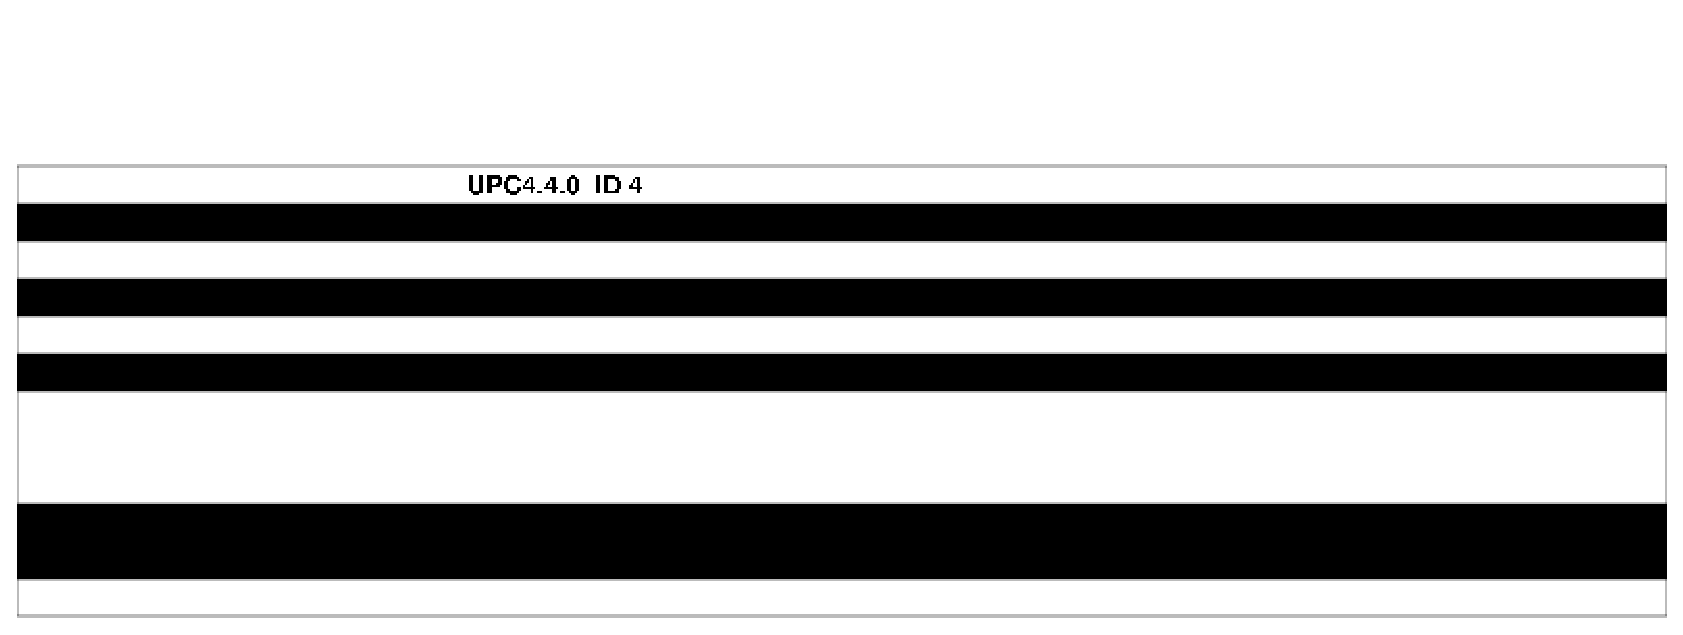
\epsfig{file=upc.eps, height=40mm}
\caption{A sample UPC barcode (one digit).}
\label{fig:upc}
\end{center}
\end{figure}

\subsection*{Synopsis}

The UPC barcode detector searches for standard, single-digit UPC
barcodes in a camera image (a sample barcode is shown above).


\subsection*{Interfaces}

\noindent Supported interfaces:
\begin{itemize}
\item {\tt blobfinder}
\end{itemize}

\noindent Required devices:
\begin{itemize}
\item {\tt camera}
\end{itemize}

%\noindent Supported configuration requests:
%\begin{itemize}
%\end{itemize}



\subsection*{Configuration file options}

TODO

\begin{center}
{\small \begin{tabularx}{\columnwidth}{|l|l|c|X|}
\hline
Name & Type & Default & Meaning\\
\hline
{\tt camera} & integer & 0 & Index of the {\tt camera} device to be used.\\
\hline
\end{tabularx}}
\end{center}

\subsection*{Notes}

For more information on the {\tt upcbarcode} driver, ask Andrew Howard:
{\tt ahoward@usc.edu}.


\newdriverex{vfh}{\cvjones}
\subsection*{Synopsis}
The {\tt VFH} driver implements the Vector Field Histogram Plus local navigation method by Ulrich and Borenstein \cite{UlrichBorenstein98}.  VFH+ provides real-time obstacle avoidance and path following capabilities for fast mobile robots.  

\subsection*{Interfaces}

\noindent Supported interfaces:

\begin{itemize}
\item {\tt position}
\end{itemize}

\noindent Required devices:
\begin{itemize}
\item {\tt position}
\item {\tt laser}
\end{itemize}

\noindent Supported configuration requests:
\begin{itemize}
\item None.
\end{itemize}


\subsection*{Configuration file options}

\begin{center}
{\small \begin{tabularx}{\columnwidth}{|l|l|c|X|}
\hline
Name & Type & Default & Meaning\\
\hline
{\tt position\_index} & integer & {\tt 0} & Index of the underlying position device.\\
{\tt laser\_index} & integer & {\tt 0} & Index of the laser device.\\
{\tt cell\_size} & length & {\tt 0.1} & Local occupancy map grid size (m).\\
{\tt window\_diameter} & integer & {\tt 61} & Dimensions of occupancy map (map consists of window\_diameter X window\_diameter cells).\\
{\tt sector\_angle} & integer & {\tt 5} & Histogram angular resolution, in degrees.\\
{\tt robot\_radius} & length & {\tt 0.25} & The radius of the robot (m).\\
{\tt safety\_dist} & length & {\tt 0.1} & The minimum distance the robot is allowed to get to obstacles (m).\\
{\tt max\_speed} & integer & {\tt 200} & The maximum allowable speed of the robot, in millimeters/second, the robot.\\
{\tt max\_turnrate} & integer & {\tt 40} & The maximum allowable turnrate of the robot.\\
{\tt free\_space\_cutoff} & float & {\tt 2000000.0} & Unitless value.  The higher the value, the closer the robot will get to obstacles before avoiding. \\
{\tt weight\_desired\_dir} & float & {\tt 5.0} & Bias for the robot to turn to move toward goal position.\\
{\tt weight\_current\_dir} & float & {\tt 3.0} & Bias for the robot to continue moving in current direction of travel.\\
{\tt distance\_epsilon} & length & {\tt 0.5} & Planar distance from
the target position that will be considered acceptable.\\
{\tt angle\_epsilon} & angle & {\tt 10 degrees} & Angular difference from
target angle that will considered acceptable.\\
\hline
\end{tabularx}}
\end{center}

\subsection*{Notes}

The primary parameters to tweak to get reliable performance are {\tt safety\_dist} and {\tt free\_space\_cutoff}.  In general, {\tt safety\_dist} determines how close the robot will come to an obstacle while turning (around a corner for instance) and {\tt free\_space\_cutoff} determines how close a robot will get to an obstacle in the direction of motion before turning to avoid.  From experience, it is recommeded that {\tt max\_turnrate} should be at least 15\% of {\tt max\_speed}.

To get initiated to VFH, I recommend setting {\tt robot\_radius} to the radius of your robot and starting with the default values for other parameters and experimentally adjusting {\tt safety\_dist} and {\tt free\_space\_cutoff} to get a feeling for how the parameters affect performance.  Once comfortable, increase {\tt max\_speed} and {\tt max\_turnrate}.  Unless you are familiar with the VFH algorithm, I don't recommend deviating from the default values for {\tt cell\_size}, {\tt window\_diameter}, or {\tt sector\_angle}.

For more information on the {\tt VFH} driver, ask Chris Jones: {\tt cvjones@robotics.usc.edu}.



\newdriverex{waveaudio}{\vaughan}
\subsection*{Synopsis}
The {\tt waveaudio} driver captures audio from /dev/dsp on systems
which support the OSS sound driver. The data is exported using the
{\tt waveform} generic sample data interface. Currently data is
captured at 8bit, mono, 16KHz.

\subsection*{Interfaces}

\noindent Supported interfaces:

\begin{itemize}
\item {\tt waveform}
\end{itemize}

\noindent Required devices:
\begin{itemize}
\item None.
\end{itemize}

\noindent Supported configuration requests:
\begin{itemize}
\item None.
\end{itemize}


\subsection*{Configuration file options}
No configuration file options are accepted.

\subsection*{Notes}
None.


\newdriverex{wavefront}{\gerkey,\ahoward}
\subsection*{Synopsis}
The {\tt wavefront} driver implements a simple path planner for a planar
mobile robot.  The underlying planner, which uses wavefront propagation,
was written by Andrew Howard; the integration into Player was done by Brian
Gerkey.

This driver works in the following way: upon receiving a new position
target, a path is planned from the robot's current pose, as reported by
the underlying localize device.  The waypoints in this path are handed
down, in sequence, to the underlying position device. By tying everything together in this way, 
this driver offers the mythical ``global goto'' for your robot.

The planner first creates a configuration space of grid cells from the map that is given, 
treating black pixels as occupied and white pixels as free. The planner assigns a cost to each of the free cells based on
their distance to the nearest obstacle. The nearer the obstacle, the higher the cost. Beyond the 
max\_radius given by the user, the cost in the c-space cells is zero.

When the planner is given a new goal, it finds a path by working its way outwards from the goal cell, assigning plan costs to the cells as it expands (like a wavefront expanding outwards in water). The plan cost in each cell is dependant on its distance from the goal, as well as the obstacle cost assigned in the configuration space step. Once the plan costs for all the cells have been evaluated, the robot can simply follow the gradient of each lowest adjacent cell all the way to the goal.

In order to function effectively with an underlying obstacle avoidance algorithm, such as Vector Field Histogram, the planner only hands off waypoints, not the entire path. The wavefront planner finds the longest straight-line distances that don't cross obstacles between cells that are on the path. The endpoints of these straight lines become sequential goal locations for the underlying device driving the robot. 

\subsection*{Interfaces}

\noindent Supported interfaces:

\begin{itemize}
\item {\tt planner}
\end{itemize}

\noindent Required devices:
\begin{itemize}
\item {\tt position}
\item {\tt localize}
\end{itemize}

\noindent Supported configuration requests:
\begin{itemize}
\item None
\end{itemize}

\subsection*{Configuration file options}

\begin{center}
{\small \begin{tabularx}{\columnwidth}{|l|l|c|X|}
\hline
Name & Type & Default & Meaning\\
\hline
{\tt position\_index} & integer & {\tt 0} & Index of the underlying position device.\\
{\tt localize\_index} & integer & {\tt 0} & Index of the underlying
localize device.\\
{\tt map\_index} & string & none & Index of the map device containing map in which
to plan.\\
{\tt map\_scale} & float & none & Meters per pixels in map.\\
{\tt robot\_radius} & length & {\tt 0.15} & Radius of robot.\\
{\tt safety\_dist} & length & {\tt robot\_radius} & Distance to keep
between robot and obstacles.\\
{\tt max\_radius} & length & {\tt 1.0} & The maximum distance from obstacles for which the planner adds additional costs for traversing\\
{\tt dist\_penalty} & float & {\tt 1.0} & Fudge factor to discourage
cutting corners.\\
{\tt dist\_epsilon} & length & {\tt 3*robot\_radius} & Distance from target
position that will be considered acceptable.\\
{\tt angle\_epsilon} & angle & {\tt 10 degrees} & Angular difference from target
angle that will be considered acceptable.\\
\hline
\end{tabularx}}
\end{center}

\subsection*{Notes}
\begin{itemize}
\item This driver is new, not widely tested, and non-trivial to configure
and use.
\item There is currently no way to get feedback from the planner, such as:
the current list of waypoints, the lack of a feasible path, or the
achievement of the final goal.
\item The underlying position device must be capable of doing position
control (i.e., not velocity control), preferably with local obstacle
avoidance (a very good candidate is the {\tt vfh} driver).
\item The underlying localize device must have already converged to a
reasonable estimate of the robot's pose before targets are sent to this
driver (otherwise results will be unpredictable at best).
\item The target thresholds ({\tt dist\_epsilon} and {\tt angle\_epsilon})
should be {\em greater} than those thresholds in the underlying position
device, assuming it's {\tt vfh}.  Otherwise, the underlying driver thinks
the robot has reached a target, while the {\tt wavefront} driver is still
waiting.
\item You must compile Player having run configure with \--enable-wavefront option in order for the planner to work
\item There are three different coordinate frames of reference you will need to deal with when using the wavefront path planner:
\begin{itemize}
\item The Stage frame of reference, which has its (0,0) origin at the (0,0) pixel of the world map, or the bottom left hand corner. Your stage world file will specify a robot's start position in these coordinates.
\item The localize frame of reference, which has (0,0) at the center of your world map. If you are giving the robot a guess as to where the robot's starting position is, you will use this frame of reference. The wavefront planner and the amcl driver use this coordinate system.
\item The robot's frame of reference, or the frame of reference for a position driver, which will have its origin (0,0) at the point where the robot starts. This means that an interface such as VFH receives goal commands with reference to that point.
\end{itemize}
\end{itemize}


\subsection*{Example: Using the  {\tt wavefront } driver with Stage and the Playernav client}

The {\tt wavefront} driver can be used together with the  amcl driver
and the vfh obstacle avoidance driver to create autonomous navigation.  The
following example illustrates its use in the Stage simulation environment with the
hospital\_section.pnm map provided with Stage. In order to visualize the path planning, this example will
use Playernav, a client written to provide a GUI to command and monitor robots, display a map and the robot localization pose. 

\begin{itemize}
\item Start up the stage simulator from the directory {\em stagedirectory}/worlds:
\begin{verbatim}
$stage hospital_section.world
\end{verbatim}
The hospital\_section.world file should contain the following:

\begin{verbatim}
bitmap
( 
  file "hospital_section.pnm" #image is 1094 x 443 pixels
  resolution .05  #this is in meters/pixel
)
gui
(
  size [1000 600] #size of gui window
  origin [30 15] #center of the screen
  scale .07 #display scale
  grid [1 10] #minor and major grid lines
  showgrid 1 
)
define simple_robot position
(
  size [ 0.4 0.4 ]
  color "red"
  shape "circle" 
  laser ()
)
simple_robot
( 
  pose [ 10 15 0 ] 
  port 6665 
)
\end{verbatim}

If this was done correctly, the stage map should come up with a robot in place

\item Start up the player server from the directory {\em player directory}/config using the following command:
\begin{verbatim}
$player -p 7000 wavefront_hospitalsection.cfg
\end{verbatim}

Where the wavefront\_hosptialsection.cfg file contains:

\begin{verbatim}
position:0 ( driver "passthrough" port 6665)
laser:0 ( driver "passthrough" port 6665)
map:0 
(
  driver "mapfile" 
  filename "stage directory/worlds/hospital_section.pnm" 
  resolution 0.05 
  negate "1"
)
localize:0
(
  driver "amcl"
  odom_index 0
  laser_index 0
  laser_map_index 0
  init_pose [-17.35 3.92 0] #This is the robot's starting position
  init_pose_var [.2 .2 10]
  alwayson 0
 )
position:2
(
  driver "vfh"
  position_index 0
  laser_index 0
  cell_size 0.1
  window_diameter 61
  sector_angle 5
  safety_dist .15
  max_speed .5
  max_turnrate 75
  free_space_cutoff  1000000.0
  weight_desired_dir 5.0
  weight_current_dir 3.0
  distance_epsilon 0.3
  angle_epsilon 10
)
planner:0
(
  driver "wavefront"
  position_index 2
  localize_index 0
  map_index 0
  safety_dist 0.15
  max_radius 1
  dist_penalty 2.0
  distance_epsilon 0.5
  angle_epsilon 20
  alwayson 0
)
\end{verbatim}

\item Now you can start the playernav client to command the robot and see the planned paths. From the directory {\em playerdirectory}/utils/playernav run:

\begin{verbatim}
$./playernav localhost:7000
\end{verbatim}

You will now get a new window with the map and the robot's position. You can drag and drop the robot with the left mouse button to 
give it a guess as to its position, but with the above configuration file, it will already be in the correct spot. Using the right mouse button
you can drag and drop the goal triangle off the robot, to the desired goal and orientation.

\end{itemize}






\newdriverex{writelog}{\ahoward}

\subsection*{Synopsis}

The {\tt writelog} driver can be used to store data from other devices
within the Player server.  The log files generated in this way can be
``replayed'' using the {\tt readlog} driver.  See the below for some
usage examples of the {\tt writelog} driver.



\subsection*{Interfaces}

The {\tt writelog} driver currently supports the {\tt null} interface,
meaning that it generates no data, and accepts no commands or
configuration requests.

Currently, the {\tt writelog} driver is capable of storing data from
the following interfaces: {\tt laser}, {\tt position}, {\tt wifi}.


\subsection*{Configuration file options}

\begin{center}
{\small \begin{tabularx}{\columnwidth}{|l|l|c|X|}
\hline
Name & Type & Default & Meaning\\
\hline
{\tt filename} & string & {\tt writelog.log} & Output log file name \\
{\tt devices} & list & none & A list of strings specifiying the
devices whose data should be stored.  Each device is specified as {\tt
``device:index''}. \\
\hline
\end{tabularx}}
\end{center}

%\subsection*{Notes}



\subsection*{Example: Storing Odometry and Laser Data}

The following configuration file will odometry from a Pioneer
and laser data from a SickLMS200 to a log file.
  \begin{verbatim}
  position:0 (driver "p2os_position")
  laser:0 (driver "sicklms200")
  null:0 
  (
    driver "writelog" 
    filename "foo.log" 
    devices ["position:0" "laser:0"]
    alwayson 1
  )
  \end{verbatim}
Note that the {\tt alwayson} flag will cause the driver to start
logging data as soon as Player is started, and will continue logging
data until Player is stopped.

Look in Section \ref{sect:readlog_driver} for an example that shows
how to replay this data using the {\tt readlog} driver.






%-----------------------------------------------------------------------------
\chapter{Architecture}
\label{chapt:architecture}
Player was designed from the beginning to be easily extended by adding
new devices and by adding new functionality to existing devices.  In fact,
Player is really a general-purpose device server; we just happen to use
it for controlling our robots.  You could use it to provide a simple, clean
interface to any sensors or actuators you have.
We describe in this chapter the overall system architecture and how
you would go about adding your own devices.  After reading this chapter,
you should consult the code for the existing devices as examples for
writing your own.  Also, keep in mind that the code may change faster than 
this document, so the details given here may not always be up to date.

\section{Server Structure}
Player is implemented in C++ and makes use of the POSIX-compliant
pthread interface for writing multi-threaded programs.   Initially, Player
was written with a very large number of threads (2 per client + 1 per device);
we found this model to be rather inefficient (especially with LinuxThreads)
and poorly scalable due to scheduler delay and context switch time.
Thus we have eliminated many threads, keeping the total thread count
constant in the number of clients.  To support code modularity and reusability
there is still generally one thread per device, though some light-weight
devices (e.g., the {\tt laserbeacon} device) do not require their own
threads.

One thread services all clients, doing the following: 
listen for new client connections on the selected TCP port(s),
read commands and requests from all current clients, 
and write data and replies to all clients.

When the server receives a request for a device that is not already setup,
it calls the proper method, {\tt Setup()}, in the object which controls the
indicated device.  The invocation of {\tt Setup()} involves spawning another
thread to communicate with that device\footnote{Most, but not all devices
have their own threads.}.  So, in total, we have 1 server thread and 1 thread
per open device.

The overall system structure of Player is shown in Figure~\ref{figure:buffers}.
The center portion of the figure is Player itself; on the left are the physical
devices and on the right are the clients.  As described above, each client
has a TCP socket connection to Player. If the client is executing on the same
host as Player, then this socket is simply a loopback connection; otherwise,
there is a physical network in between the two.  At the other end, Player
connects to each device by whatever method is appropriate for that device.
For most devices, including the laser, camera, and robot microcontroller,
Player makes this connection via an RS-232 serial line.  However, connections
to the ACTS vision server and Festival speech synthesizer are via a TCP socket.

Within Player, the various threads communicate through a shared global
address space.  As indicated in Figure~\ref{figure:buffers}, each
device has associated with it a command buffer and a data buffer.
These buffers, which are each protected by mutual exclusion locks,
provide an asynchronous communication channel between the device
threads and the client reader and writer threads.  For example, when
the client reader thread receives a new command for a device,
it writes the command into the command buffer for that device.  At
some later point in time, when the device thread is ready for a new
command, it will read the command from its command buffer and send
it on to the device.  Analogously, when a device thread receives
new data from its device, it writes the data into its data
buffer.  Later, when the client writer thread is ready to send new
data from that device to a particular client, it reads the data from the data
buffer and passes it on to the client.  In this way, the client
service thread is decoupled from the device service threads (and
thus the clients are decoupled from the devices).  Also, just by the
nature of threads, the devices are decoupled from each other.

\begin{figure}[t]
 \centering
 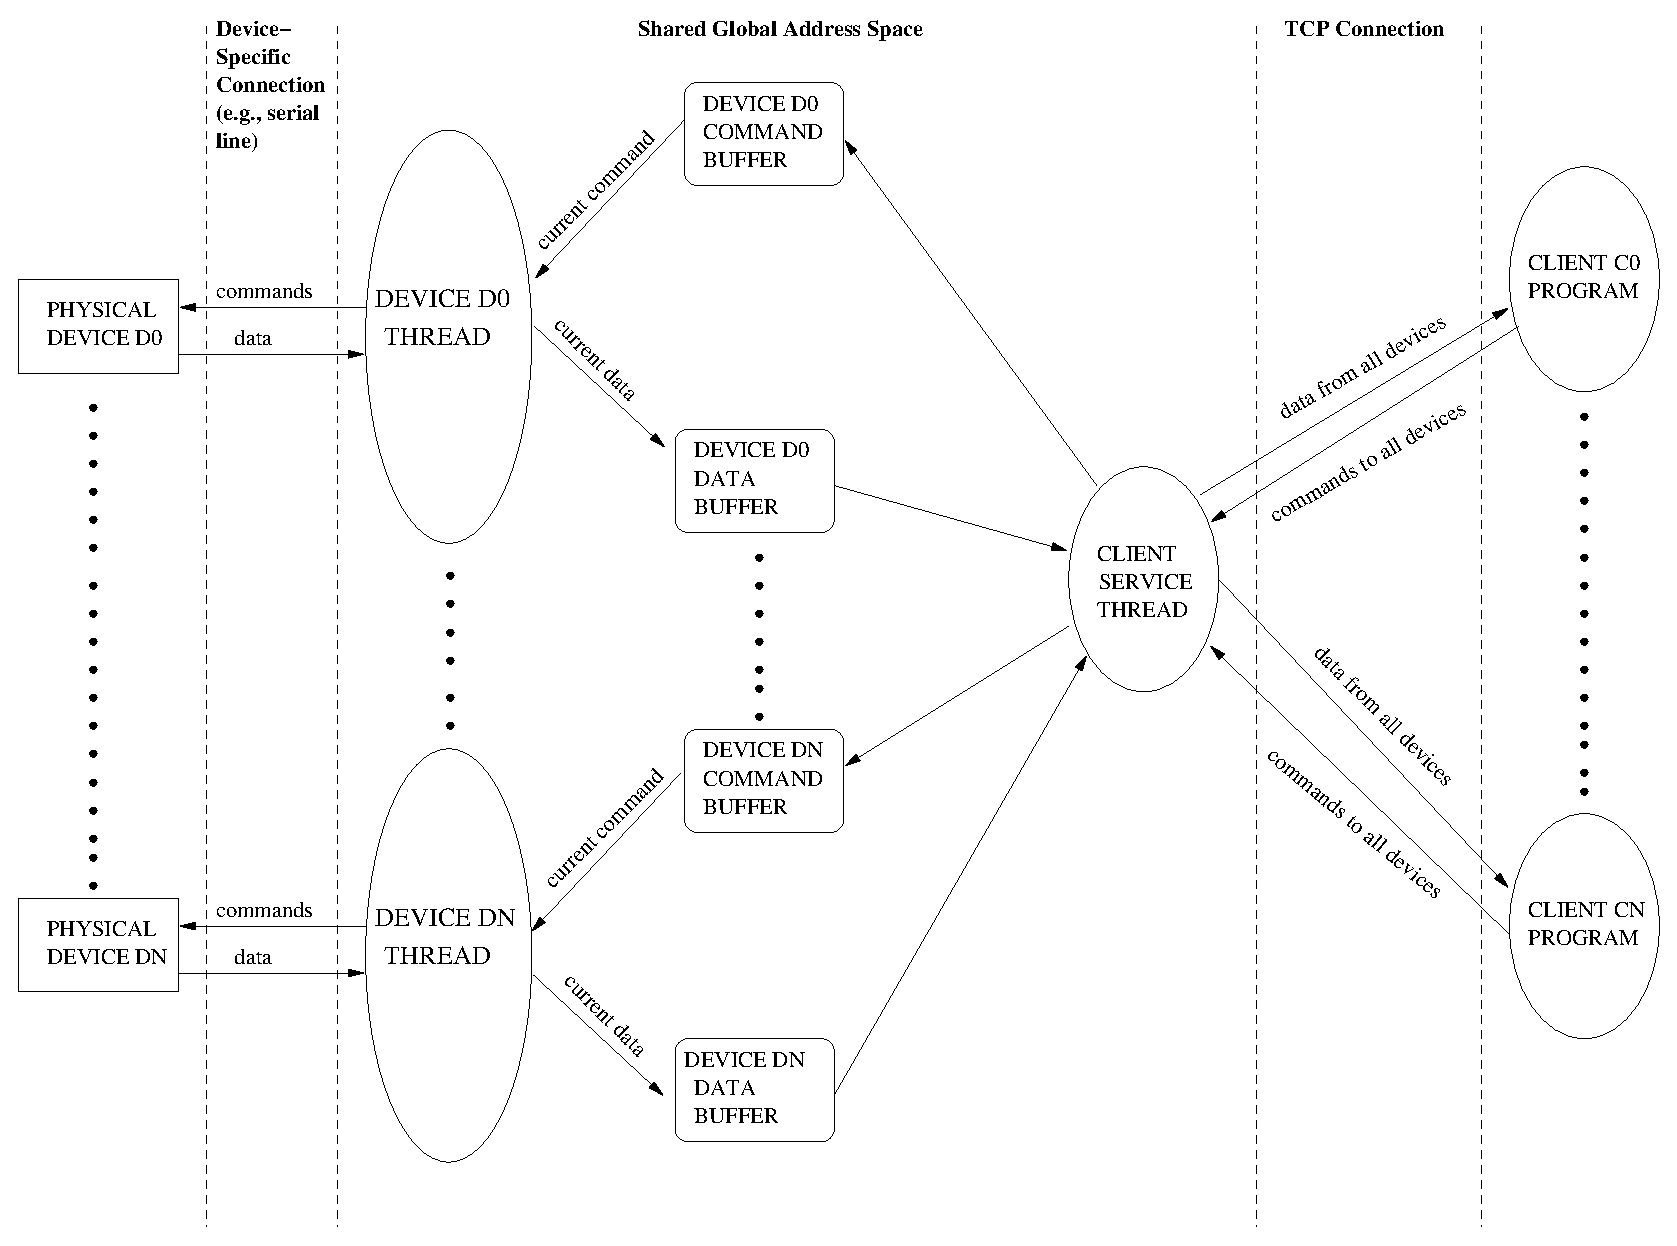
\epsfig{file=buffers.eps, width=0.900\textwidth}
  \caption{{\em Overall system architecture of Player}}
  \label{figure:buffers}
\end{figure} 

\subsection{Device data}
By default, each client will receive new data from each device to which it is
subscribed at 10Hz.  Of course, receiving data at 10Hz may not be reasonable
for all clients; thus we provide a method for changing the frequency, and
also for placing the server in a request/reply mode.  It is important to
remember that even when a client receives data slowly, there is no backlog
and it always receives the most current data; it has simply missed out on
some intervening information.  Also, these frequency changes affect the
server's behavior with respect to each client individually; the client at
30Hz and the client at 5Hz can be connected simultaneously, and the server
will feed each one data at its preferred rate.

There are four (per-client) modes of data delivery, as follows:
\begin{itemize}
\item {\tt PLAYER\_DATAMODE\_PUSH\_ALL} : periodically send to the client
current data from all devices currently opened for reading
\item {\tt PLAYER\_DATAMODE\_PULL\_ALL} : on request from the client, send it
current data from all devices currently opened for reading
\item {\tt PLAYER\_DATAMODE\_PUSH\_NEW} : periodically send to the client
current data only from those devices that are opened for reading and
have generated new data since the last cycle
\item {\tt PLAYER\_DATAMODE\_PULL\_NEW} : on request from the client, send it 
current data only from those devices that are opened for reading and
have generated new data since the last cycle
\end{itemize}
The default mode is currently {\tt PLAYER\_DATAMODE\_PUSH\_NEW}, which many
clients will find most useful. In general, the {\tt *PUSH*} modes, which
essentially provide continuous streams of data, are good when implementing
simple (or multi-threaded) client programs in which the process will
periodically block on the socket to wait for new data.  Likewise, the {\tt
*PULL*} modes are good for client programs that are very slow and/or aperiodic.
Along the other dimension, the {\tt *NEW*} modes are most efficient, as they
never cause ``old'' data to be sent to the client.  However, if a client
program does not cache sensor data locally, then it might prefer to use one
of the {\tt *ALL*} modes in order to receive all sensor data on every cycle;
in this way the client can operate each cycle on the sensor data in place
as it is received.

Of course, it is possible for a device to generate new data faster than
the client is reading from the server.  In particular, there is no method
by which a device can throw an interrupt to signal that it has data ready.
Thus the data received by the client will always be slightly older for having
sat inside the shared data buffer inside Player.  This ``buffer sit'' time
can be minimized by increasing the frequency with which the server is sending
data to the client\footnote{On Linux, due to the 10ms scheduler granularity,
the effective upper limit on data rate is 50Hz.}.  In any case, all data
is timestamped by the originating device driver, preferably as close to
the time when the data was gathered from the device.  This data timestamp
is generally a very close approximation to the time at which the sensed
phenomenon occurred and can be used by client programs requiring (fairly)
precise timing information.

\subsection{Device commands}
Analogous to the issue of data freshness is the fact that there is no guarantee
that a command given by a client will ever be sent to the intended physical
device.  Player does not implement any device locking, so when multiple
clients are connected to a Player server, they can simultaneously write into
a single device's command buffer.  There is no queuing of commands, and each
new command will overwrite the old one; the service thread for the device
will only send to the device itself whatever command it finds each time
it reads its command buffer.  We chose not to implement locking in order
to provide maximal power and flexibility to the client programs.  In our
view, if multiple clients are concurrently controlling a single device,
such as a robot's wheels, then those clients are probably cooperative,
in which case they should implement their own arbitration mechanism at a
higher level than Player.  If the clients are not cooperative, then the
subject of research is presumably the interaction of competitive agents,
in which case device locking would be a hindrance.

\subsection{Device configurations}
Whereas the data and command for each device are stored in simple buffers that
are successively overwritten, configuration requests and replies are stored
in queues.  Configuration requests, which are sent from client to server,
are stored in the device's incoming queue.  Configuration replies, which
are sent from server to client, are stored in the device's outgoing queue.
These queues are fixed-size: queue element size is currently fixed at 1KB
for all devices and queue length is determined at compile-time by each
device's contructor.

\section{Adding a new device driver}
Having described the internal workings of Player, we now give a short
tutorial on how you would go about extending the server by adding a new
device driver.  As mentioned earlier, in lieu of a more complete prescription 
for creating drivers, an examination of the code for the existing drivers 
should provide you with sufficient examples.  You should be familiar with C++,
class inheritance, and thread programming.

The first step in adding a new driver to Player is to decide which
interface(s) it will support.  The existing interfaces are described in
Chapter~\ref{chapt:interfaces} and their various message structures and
constants are defined in {\tt include/player.h}.  Although you can create a
new interface, you should try to fit your driver to an existing interface,
of which there are many.  By deciding to support an existing interface,
you'll have less work to do in the server, and will likely have instant
client support for your driver in several languages.

To create a new driver, you should create a new class for the driver, which
should inherit from {\tt CDevice}, declared in {\tt server/device.h} and
implemented in {\tt server/device.cc}.  That base class defines a standard
interface, part of which the new driver must implement (other parts it
may choose to override).  We now describe the salient aspects of the {\tt
CDevice} class.

\subsection{Constructors}
There are two {\tt CDevice} constructors available.  Most drivers will
use the more expressive of the two:
\begin{verbatim}
    CDevice::CDevice(size_t datasize, size_t commandsize, 
                     int reqqueuelen, int repqueuelen);}
\end{verbatim}
Arguments are:
\begin{itemize}
\item {\tt datasize} : the size (in bytes) of the buffer to be allocated to 
hold the current data from the driver
\item {\tt commandsize} : the size (in bytes) of the buffer to be allocated to 
hold the current command for the driver
\item {\tt reqqueuelen} : the length (in number of elements) of the queue 
to be allocated to hold incoming configuration requests for the driver
\item {\tt repqueuelen} : the length (in number of elements) of the queue to 
be allocated to hold outgoing configuration replies from the driver
\end{itemize}
All requested buffers and queues will be allocated by the {\tt CDevice}
constructor (we describe below where the pointers are stored in the object).
This constructor should be  invoked in the preamble to the driver's own
constructor; for example, the {\tt sicklms200} driver, which produces 
fixed-length data, accepts no commands, and uses incoming and outgoing 
configuration queues both of length 1, has a constructor that begins:
\begin{verbatim}
    CLaserDevice::CLaserDevice(int argc, char** argv) : 
      CDevice(sizeof(player_laser_data_t),0,1,1)
\end{verbatim}

Now, you may want to allocte your own buffers and/or queues (e.g.,
CStageDevice does its own memory management in static {\tt mmap()}ed
segments).  If so, then your driver should not invoke a {\tt CDevice}
constructor; the ``default'' zero-argument constructor will be invoked for you
and will properly initialize some class members.  Even if you do allocate your
own buffers, you might benefit from letting {\tt CDevice} know where they are,
in that you could still use the standard {\tt CDevice} methods (described
below) to interface with your driver.  You can do this by calling (usually in
your own constructor) {\tt SetupBuffers()}:
\begin{verbatim}
    void CDevice::SetupBuffers(unsigned char* data, size_t datasize, 
                               unsigned char* command, size_t commandsize, 
                               unsigned char* reqqueue, int reqqueuelen, 
                               unsigned char* repqueue, int repqueuelen);
\end{verbatim}
Arguments are:
\begin{itemize}
\item {\tt data} : the buffer allocated to hold the current data from the
driver
\item {\tt datasize} : the size (in bytes) of {\tt data}
\item {\tt command} : the buffer allocated to hold the current command for the 
driver
\item {\tt commandsize} : the size (in bytes) of {\tt command}
\item {\tt reqqueue} : the buffer allocated to hold incoming configuration
requests; it should be an allocated as an array of {\tt playerqueue\_elt\_t}s
\item {\tt reqqueuelen} : the length (in number of elements) of {\tt reqqueue}
\item {\tt repqueue} : the buffer allocated to hold outgoing configuration
replies; it should be an allocated as an array of {\tt playerqueue\_elt\_t}s
\item {\tt repqueuelen} : the length (in number of elements) of {\tt repqueue}
\end{itemize}
In this case, {\tt SetupBuffers()} will allocate {\tt PlayerQueue} objects
to handle configurations; they will operate on the memory segments that you 
provide.

Whether you let the {\tt CDevice} constructor allocate your buffers or do it
yourself and then call {\tt SetupBuffers()}, the relevant pointers and sizes
are stored in the following protected members of {\tt CDevice}:
\begin{verbatim}
    // buffers for data and command
    unsigned char* device_data;
    unsigned char* device_command;

    // maximum sizes of data and command buffers
    size_t device_datasize;
    size_t device_commandsize;

    // amount at last write into each respective buffer
    size_t device_used_datasize;
    size_t device_used_commandsize;
    
    // queues for incoming requests and outgoing replies
    PlayerQueue* device_reqqueue;
    PlayerQueue* device_repqueue;
\end{verbatim}

\subsection{Locking access to buffers}
Because Player is a multi-threaded program, all access to shared buffers
must be protected by mutual exclusion locks.  For this purpose, {\tt CDevice}
contains a (private) {\tt pthread\_mutex\_t}, and provides (protected) {\tt
Lock()} and {\tt Unlock()} methods that call {\tt pthread\_mutex\_lock()}
and {\tt pthread\_mutex\_unlock()}, respectively (these methods are virtual;
thus a driver can override them in order to use a different mutual exclusion
mechanism).  You should surround all accesses to any of a driver's shared
buffers or queues with calls to {\tt Lock()} and {\tt Unlock()}.  The default
interface methods described in the following sections do exactly this.

\subsection{Instantiation}
\label{sect:instantiation}
Because Player supports multiple indexed instances of devices, your driver
should be prepared to be multiply instantiated (e.g., you generally
should not use global or other static variables) and you must provide
a function for instantiating it.  When a new instance of a driver is
required, Player will call an appropriate instantiation function (see
Section~\ref{sect:register-device} for how to register your instantiation
method).  This function should return (as a {\tt CDevice*}) a pointer to a
new instance of your device class.  Since an object has not yet been created
when this function is called, it must be declared outside of the class
(or static within the class).
This function should match the following prototype:
\begin{verbatim}
  CDevice* Foo_Init(char* interface, ConfigFile* cf, int section);
\end{verbatim}
The arguments are:
\begin{itemize}
\item {\tt interface}: the string name of the interface that the driver has
been requested to support
\item {\tt cf}: a object containing information gleaned from the user's
configuration file
\item {\tt section}: in which section of the configuration file your driver 
was requested
\end{itemize}
You should check the requested {\tt interface} to be sure that your driver can
support it.  If you cannot, then return {\tt NULL}.  You should look in
the configuration file object {\tt cf} for any options that may have been
specified for you driver (look at existing drivers and {\tt
server/configfile.h} for how to get options out).

\subsection{Setup}
When the first client subscribes to a device, the driver's {\tt Setup()}
method is called.  This method is set to NULL in CDevice:
\begin{verbatim}
    virtual int CDevice::Setup() = 0;
\end{verbatim}
Thus every driver {\em must} implement this method.  After doing whatever is
required to initialize the device (e.g., open a serial port and spawn a thread
to interact with it), {\tt Setup()} should return either zero to indicate that
the device was successfully setup, or non-zero to indicate that setup failed.
Since clients may immediately request data and since they may never send 
commands, a driver's data buffer and command buffer should be sensibly
``zeroed'' in {\tt Setup()}.

\subsection{Shutdown}
When the last client unsubscribes from a device, the driver's 
{\tt Shutdown()} method is called.  This method is set to NULL in CDevice:
\begin{verbatim}
    virtual int CDevice::Shutdown() = 0;
\end{verbatim}
Thus every driver {\em must} implement this method.  After doing whatever
is required to stop the device (e.g., kill a thread and close a serial
port), {\tt Shutdown()} should return either zero to indicate that device was
successfully shutdown, or non-zero to indicate that shutdown failed.

\subsection{Thread management}
In order to leverage parallelism, most (but not all) devices use separate
threads to do their work.  Because thread creation is not intuitively
compatible with C++ object context, some support is provided in {\tt CDevice}
for starting and stopping threads.  You are not required to use this support,
but you might find it useful.

The first step is to define in your class a public method {\tt Main()} that
overrides the virtual declaration:
\begin{verbatim}
    virtual void CDevice::Main();
\end{verbatim}
Presumably your definition of {\tt Main()} will contain a loop that executes
all device interaction.  When you want to start your thread (probably in {\tt
Setup()}), call {\tt StartThread()}.  A new thread will be created;
in that thread your driver's {\tt Main()} method will be invoked, with the
proper context of your driver's object.  When you want to stop your thread
(probably in {\tt Shutdown()}), call {\tt StopThread()}, which will cancel and
join your thread; thus your thread should respond to cancellation requests
(even if it initially defers them) and should be in a joinable state (i.e., it
should {\em not} be detached).

\subsection{Data access methods}
{\em Most drivers can use the default {\tt CDevice} implementations of the
following methods; however, they are virtual and can be overridden if
necessary.}

\subsubsection{PutData}
Whenever your driver has new data, it should call {\tt PutData()}:
\begin{verbatim}
    virtual void CDevice::PutData(unsigned char* src, size_t len,
                         uint32_t timestamp_sec, uint32_t timestamp_usec);
\end{verbatim}
Arguments are:
\begin{itemize}
\item {\tt src} : pointer to the new data
\item {\tt len} : length (in bytes) of the new data
\item {\tt timestamp\_sec} : the time at which the new data was produced
\item {\tt timestamp\_usec} : the time at which the new data was produced
\end{itemize}
The default implementation of {\tt PutData()} will {\tt Lock()} access,
{\tt memcpy()} your new data into {\tt device\_data}, save your {\tt len} and
timestamp,  and {\tt Unlock()} access.  If {\tt ts} is {\tt NULL}, then
{\tt PutData()} will use the current time (either system or simulator,
as appropriate).

\subsubsection{GetNumData}
When a client wants to read data from your driver, the server will first
call {\tt GetNumData()}:
\begin{verbatim}
    virtual size_t GetNumData(void* client);
\end{verbatim}
Arguments are:
\begin{itemize}
\item {\tt client} : a unique id for who wants the data
\end{itemize}
This method should return the number of data packets that are ready for the
given client at this time.  The server will then call {\tt GetData()} that
many times.  The default implementation of {\tt GetNumData()} simply returns
1, which is almost always the right thing.  However, your driver can override
this method if you want.

\subsubsection{GetData}
When a client wants to read data from your driver, the server will 
invoke {\tt GetData()}:
\begin{verbatim}
    virtual size_t GetData(void* client, unsigned char* dest, size_t len,
                        uint32_t* timestamp_sec, uint32_t* timestamp_usec);
\end{verbatim}
Arguments are:
\begin{itemize}
\item {\tt client} : a unique id for who wants the data
\item {\tt dest} : pointer to a buffer into which to copy the data
\item {\tt len} : length (in bytes) of {\tt dest}
\item {\tt timestamp\_sec} : buffer into which to copy the time at which the data was 
\item {\tt timestamp\_usec} : buffer into which to copy the time at which the data was 
produced
\end{itemize}
The default implementation of {\tt GetData()} will {\tt Lock()} access, {\tt
memcpy()} data from {\tt device\_data} into {\tt dest} (up to {\tt len}
bytes), retrieve timestamp information, {\tt Unlock()} access, and return 
how many bytes of data were copied.

\subsection{Command access methods}
{\em Most devices can use the default {\tt CDevice} implementations of the
following methods; however, they are virtual and can be overridden if
necessary.}

\subsubsection{PutCommand}
When a client sends a new command for your device, the server will
invoke {\tt PutCommand()}:
\begin{verbatim}
    virtual void PutCommand(void* client, unsigned char* src, size_t len);
\end{verbatim}
Arguments are:
\begin{itemize}
\item {\tt client} : a unique id for the source of the command
\item {\tt src} : pointer to the new command
\item {\tt len} : length (in bytes) of the new command
\end{itemize}
The default implementation of {\tt PutCommand()} will {\tt Lock()} access,
{\tt memcpy()} the new command into {\tt device\_command}, save {\tt len},
and {\tt Unlock()} access.

\subsubsection{GetCommand}
When you want the current command for your device, you should call 
{\tt GetCommand()}:
\begin{verbatim}
    virtual size_t CDevice::GetCommand(unsigned char* dest, size_t len);
\end{verbatim}
Arguments are:
\begin{itemize}
\item {\tt dest} : pointer to a buffer into which to copy the command
\item {\tt len} : length (in bytes) of {\tt dest}
\end{itemize}
The default implementation of {\tt GetCommand()} will {\tt Lock()} access, 
{\tt memcpy()} the command from {\tt device\_command} into {\tt dest} 
(up to {\tt len} bytes), {\tt Unlock()} access, and return how many bytes of 
command were copied.

\subsection{Configuration access methods}
{\em Most drivers can use the default {\tt CDevice} implementations of the
following methods; however, they are virtual and can be overridden if
necessary.}

\subsubsection{PutConfig}
When a new configuration request arrives for your device, the server will
invoke {\tt PutConfig()}:
\begin{verbatim}
    virtual int CDevice::PutConfig(player_device_id_t* device, 
                                   void* client, 
                                   void* data,
                                   size_t len);
\end{verbatim}
Arguments are:
\begin{itemize}
\item {\tt device} : an identifier that indicates the device for whom the
request is intended
\item {\tt client} : a tag that will be used to route the reply back to the
right client (or other device)
\item {\tt data} : buffer containing the new request
\item {\tt len} : length (in bytes) of the new request
\end{itemize}
The default implementation of {\tt PutConfig} will {\tt Lock()} access, 
push the request onto {\tt device\_reqqueue}, and {\tt Unlock()} access.  If
all is well, then zero is returned; otherwise (e.g., if the queue is full)
non-zero is returned and the server will send an error response message to the
waiting client.

\subsubsection{GetConfig}
To check for new configuration requests in your device, you should call
{\tt GetConfig()}:
\begin{verbatim}
    virtual size_t CDevice::GetConfig(player_device_id_t* device, 
                                      void** client, 
                                      void *data, 
                                      size_t len);
\end{verbatim}
Arguments are:
\begin{itemize}
\item {\tt device} : an identifier that indicates the device for whom the
request is intended (useful when one queue is used for multiple devices,
as is the case with P2OS)
\item {\tt client} : a place to store a tag that will be used to route the 
reply back to the right client (or other device)
\item {\tt data} : buffer into which to copy the new request
\item {\tt len} : length (in bytes) of {\tt data}
\end{itemize}
For convenience, there is also a short form of {\tt GetConfig()}:
\begin{verbatim}
    virtual size_t CDevice::GetConfig(void** client,
                                      void* data,
                                      size_t len);
\end{verbatim}
The default implementation of {\tt GetConfig} will {\tt Lock()} access, 
pop a request off {\tt device\_reqqueue}, and {\tt Unlock()} access.  If
there was a request to be popped then the size of the request is returned;
otherwise zero is returned, indicating that there are no pending requests.
If there is request then hang onto {\tt client} because you will need to pass 
it back in {\tt PutReply()}.

\subsubsection{PutReply}
After servicing a request, you must generate an appropriate reply; you do this
by calling {\tt PutReply()}:
\begin{verbatim}
    virtual int CDevice::PutReply(player_device_id_t* device, 
                                  void* client, 
                                  unsigned short type, 
                                  struct timeval* ts, 
                                  void* data, 
                                  size_t len);
\end{verbatim}
Arguments are:
\begin{itemize}
\item {\tt device} : an identifier that indicates from which the device the
reply comes (useful when one queue is used for multiple devices,
as is the case with P2OS)
\item {\tt client} : the tag that you received in {\tt GetConfig}
\item {\tt type} : the type of the reply (see below)
\item {\tt ts} : pointer to time at which the configuration was executed
\item {\tt data} : the reply itself (if any)
\item {\tt len} : length (in bytes) of {\tt data}
\end{itemize}
There are also two short forms of {\tt PutReply()}:
\begin{verbatim}
    virtual int CDevice::PutReply(void* client, 
                                  unsigned short type, 
                                  struct timeval* ts, 
                                  void* data, 
                                  size_t len);

    virtual int CDevice::PutReply(void* client, 
                                  unsigned short type);
\end{verbatim}
The first short form assumes that the caller is the originator of the reply.
The second short form further assumes that the reply is zero-length and
that it should be stamped with the current time.

The default implementation of {\tt PutReply} will {\tt Lock()} access,
push the reply onto {\tt device\_repqueue}, and {\tt Unlock()} access.
If the reply queue is full (which should not happen in practice) then -1
is returned; otherwise a non-negative integer is returned.  The given {\tt
type} will be used as the message type for the reply that will be sent to
the client; it should be one of:
\begin{itemize}
\item {\tt PLAYER\_MSGTYPE\_RESP\_ACK} : the configuration was successful
\item {\tt PLAYER\_MSGTYPE\_RESP\_NACK} : the configuration failed
\end{itemize}
If {\tt ts} is {\tt NULL}, then the current time is filled in.  Zero-length
replies are valid (and frequent).

\subsubsection{GetReply}
The server will periodically check for replies from your device by calling
{\tt GetReply()}:
\begin{verbatim}
    virtual int CDevice::GetReply(player_device_id_t* device, 
                                  void* client, 
                                  unsigned short* type, 
                                  struct timeval* ts, 
                                  void* data, 
                                  size_t len);
\end{verbatim}
Arguments are:
\begin{itemize}
\item {\tt device} : an identifier indicating from which the device the reply
has come
\item {\tt client} : a tag to be matched 
\item {\tt type} : place to copy the type of the reply
\item {\tt ts} : place to copy the time at which the configuration was executed
\item {\tt data} : buffer into which to copy the reply
\item {\tt len} : length (in bytes) of {\tt data}
\end{itemize}
The default implementation of {\tt GetReply()} will {\tt Lock()} access,
pop a reply off {\tt device\_repqueue}, {\tt Unlock()} access, and return the
length of the reply.  Because zero-length replies are valid, {\tt GetReply()}
will return -1 to indicate that no reply is available.

\subsection{Registering your device}
\label{sect:register-device}
In order to inform the server about the availability of your driver,
you must add it to {\tt driverTable}, a global table of drivers
that may be instantiated.  You should add your driver by calling {\tt
AddDevice()} in the function {\tt register\_devices()}, declared in {\tt
server/deviceregistry.cc}:  
\begin{verbatim}
    int AddDriver(char* name, char access, 
                  CDevice* (*initfunc)(char*,ConfigFile*,int));
\end{verbatim}
Arguments are:
\begin{itemize}
\item {\tt name} : the name of your driver
\item {\tt access} : the allowable access mode for your driver; should be
one of:
\begin{itemize}
\item {\tt PLAYER\_READ\_MODE}
\item {\tt PLAYER\_WRITE\_MODE}
\item {\tt PLAYER\_ALL\_MODE}
\end{itemize}
\item {\tt initfunc} : a function that can be used to create
a new instance of your device (see Section~\ref{sect:instantiation})
\end{itemize}
You may find it convenient to write a registration function, e.g.:
\begin{verbatim}
  void SickLMS200_Register(DriverTable* table)
  {
    table->AddDriver("sicklms200", PLAYER_READ_MODE, SickLMS200_Init);
  }
\end{verbatim}
You should also {\tt \#include} your device's class header in {\tt
deviceregistry.cc}.   To encourage modularity of the server by allowing
drivers to be left out at compile-time, it is customary to make both the
{\tt \#include} and  {\tt AddDriver()} conditioned on compiler directives.
For example:
\begin{verbatim}
    #ifdef INCLUDE_SICK
    void SickLMS200_Register(DriverTable* table);
    #endif

    ...


    void
    register_devices()
    {
      ...

      #ifdef INCLUDE_SICK
        SickLMS200_Register(driverTable);
      #endif

      ...
    }
\end{verbatim}

\subsection{Compiling your device}
\label{sect:compilation}
Finally, you need to compile your device and link it into the server binary.
You really need to know something about GNU Autotools to do this.  As such,
look at how the existing drivers are linked in.


\subsection{Building a shared library}
\label{sect:shared-lib}
As an alternative to statically linking your device driver directly into the
Player binary, you can build your driver as a shared object and have Player
load it at run-time.  If you choose to take this path, then you should still
follow most of the directions given in the previous sections, except for the
registration and compilation details in 
Sections~\ref{sect:register-device}--\ref{sect:compilation}.

Instead of registering your device in {\tt deviceregistry.cc}, you should
do so in an initialization function that will be invoked by the loader.
You must declare this initialization function, as well as a finalization
function, in your driver code.  For example, in order to build the {\tt
sicklms200} driver as a shared object, the following code is added 
to {\tt sicklms200.cc}:
\begin{verbatim}
    #include <drivertable.h>
    extern DriverTable* driverTable;
    
    /* need the extern to avoid C++ name-mangling  */
    extern "C" {
    void _init(void)
    {
      driverTable->AddDriver("sicklms200", PLAYER_READ_MODE, SickLMS200_Init);
    }
    
    void _fini(void)
    {
      /* probably don't need any code here; the destructor for the device
       * will be called when Player shuts down.  this function is only useful
       * if you want to dlclose() the shared object before Player exits
       */
    }
    }
\end{verbatim}
The {\tt \_init()} function will be invoked by the loader when Player
calls {\tt dlopen()} to load your driver.  The {\tt \_fini()} function
will be invoked when the library is {\tt dlclose()}ed; however, Player never
closes your library explicitly, so {\tt \_fini()} will be called when Player
exits.

The details of building a shared object vary from system to system, but the
following example, which works with g++ on Linux, should get you started:
\begin{verbatim}
    $ g++ -Wall -DPLAYER_LINUX -g3 -I$PLAYER_DIR/server -c sicklms200.cc
    $ g++ -shared -nostartfiles -o sicklms200.so sicklms200.o
\end{verbatim}
Having built your driver library, tell Player on the command-line to load it
(as described in Section~\ref{sect:commandline}), e.g.:
\begin{verbatim}
    $ player -d sicklms200.so
\end{verbatim}

Note that the dynamic loading functionality is still somewhat experimental,
and is not currently used by any core Player drivers.  However, it should
work.  If you use shared libraries, please let us know about your experiences.


\bibliographystyle{plain}
\bibliography{player}

\appendix
%-----------------------------------------------------------------------------
\chapter{The C Client Interface}
\label{app:c}
Included with Player is a simple, no-frills client interface library
written in ANSI C ({\tt client\_libs/c}).  This client is 
intentionally primitive and most users
will find it inconvenient for writing anything more that the simplest
control program.  Rather than direct use, the C client should be considered
the reference implementation of a Player client library and should be
consulted for networking details when writing new clients in other 
languages (the C client can also be used directly as a low-level substrate 
for other clients; the C++ client is implemented in this way).
In the file {\tt playercclient.c} are defined the 5
device-neutral functions necessary in any client:
\begin{itemize}
\item {\tt player\_connect()} : connect to the server
\item {\tt player\_disconnect()} : disconnect from the server
\item {\tt player\_read()} : read one data packet from the server
\item {\tt player\_write()} : write one command packet to the server
\item {\tt player\_request()} : send a request packet and wait for the reply
\end{itemize}
In addition, the {\em very} useful helper function 
{\tt player\_request\_device\_access()} (a special case of 
{\tt player\_request()} that obtains access to devices) is defined.

In the files {\tt print.c} and {\tt helpers.c} are defined some
device-specific functions that simplify direct use of the C client; we do
not document them here.

\section{Debug Information}
Before getting to the core functions of the C client, we note that they
can each generate some debug information to {\tt stderr}.  This 
information is generally helpful, especially in diagnosing problems; you 
should probably not disable it.  However, a function is provided for 
adjusting the amount of debug information that is printed:

{\small
\begin{verbatim}
  /*
   * use this to turn off debug ouput.
   *
   * higher numbers are more output, 0 is none.
   *
   * incidentally, if <level> is -1, it returns the current level and
   * the current level is unchanged
   */
  int player_debug_level(int level);
\end{verbatim}}

The default debug level is 5, which prints all messages.  This
same function is used to vary the debug output from the C++ client, since
it is built on top of the C client.


\section{Connecting to the Server}
The C client makes no use of static data structures for maintaining connection
information; rather the user must always supply a pointer to a properly
initialized connection structure, of type {\tt player\_connection\_t}.
This structure is initialized by {\tt player\_connect()}:

{\small
\begin{verbatim}
  /*
   * connects to server listening at host:port.  conn is filled in with
   * relevant information, and is used in subsequent player function
   * calls
   *
   * Returns:
   *    0 if everything is OK (connection opened)
   *   -1 if something went wrong (connection NOT opened)
   */
  int player_connect(player_connection_t* conn, const char* host, int port);
\end{verbatim}
}

Note that the connection will be blocking.  A simple example:

{\small
\begin{verbatim}
  ...
  player_connection_t conn;

  /* Connect to Player server */
  if(player_connect(&conn, "localhost", PLAYER_PORTNUM))
    exit(1);
  ...
\end{verbatim}
}

\section{Requesting Device Access}
To ease the common process of requesting read and write access to devices,
the C client includes the function {\tt player\_request\_device\_access()}:

{\small
\begin{verbatim}
  ...
  /*
   * issue a single device request (special case of player_request())
   *
   * 
   * if grant_access is non-NULL, then the actual granted access will
   * be written there.
   *
   *   Returns:
   *      0 if everything went OK
   *     -1 if something went wrong (you should probably close the
   *     connection!)
   */
  int player_request_device_access(player_connection_t* conn,
                                   uint16_t device,
                                   uint16_t device_index,
                                   uint8_t req_access,
                                   uint8_t* grant_access);
\end{verbatim}
}


The following  code fragment obtains 'all' ({\tt 'a'}) access to the 
{\tt ptz} device.

{\small
\begin{verbatim}
  ...
  /* Request 'all' access to the ptz device */
  if(player_request_device_access(&conn, PLAYER_PTZ_CODE, 0, 'a',NULL) == -1)
    exit(1);
  ...
\end{verbatim}
}

\section{Reading Data}
For obtaining data from devices, the C client provides the rather simple 
function {\tt player\_read()}:

{\small
\begin{verbatim}
  /*
   * read from the indicated connection.  put the data in buffer, up to
   * bufferlen.
   *
   * Returns:
   *    0 if everything went OK
   *   -1 if something went wrong (you should probably close the connection!)
   */
  int player_read(player_connection_t* conn, player_msghdr_t* hdr,
                  char* payload, size_t payloadlen);
\end{verbatim}
}

This function will read one data packet from the server, blocking 
if no packet is available.  It is the caller's responsibility to 
provide sufficient storage for the header and payload, and
{\tt player\_read()} will not overrun the provided buffers.  After
calling {\tt player\_read()}, the user will presumably examine the fields
of the header in order to know how to process the payload.  Note that 
{\tt player\_read()} will appropriately byte-swap all fields in the header,
but will not transform the contents of the payload in any way.  A simple
example:

{\small
\begin{verbatim}
  ...
  player_msghdr_t hdr;
  char data[PLAYER_MAX_MESSAGE_SIZE];

  if(player_read(&conn, &hdr, data, sizeof(data)) == -1)
    exit(1);
  ...
\end{verbatim}
}

\section{Writing Commands}
For writing commands to devices, the C client provides the function
{\tt player\_write()}:

{\small
\begin{verbatim}
  /*
   * write commands to the indicated connection. writes the data contained
   * in command, up to commandlen.
   *
   * Returns:
   *    0 if everything goes OK
   *   -1 if something went wrong (you should probably close the connection!)
   */
  int player_write(player_connection_t* conn, 
                   uint16_t device, uint16_t device_index,
                   const char* command, size_t commandlen);
\end{verbatim}
}

This function will build the appropriate message header, including
appropriate byte-swapping of the fields.  The first {\tt commandlen}
bytes of {\tt command} will be copied in as the payload of a messge that
will be sent to the server.  Note that the caller must byte-swap
the contents of the command itself.  A simple example that tells the
0th {\tt position} device to spin in place:

{\small
\begin{verbatim}
  ...
  player_position_cmd_t cmd;
  cmd.speed = htons(0);
  cmd.turnrate = htons(40);
  if(player_write(&conn, PLAYER_POSITION_CODE, 0, (char*)&cmd, 
                  sizeof(player_position_cmd_t)) == -1)
    exit(1);
  ...
\end{verbatim}
}

\section{Requesting Configuration Changes}
For requesting configuration changes to devices, the C client provides
the function {\tt player\_request()}:

{\small
\begin{verbatim}
  /*
   * issue some request to the server. requestlen is the length of the 
   * request.  reply, if non-NULL, will be used to hold the reply; replylen
   * is the size of the buffer (player_request() will not overrun your buffer)
   *
   *   Returns:
   *      0 if everything went OK
   *     -1 if something went wrong (you should probably close the connection!)
   */
  int player_request(player_connection_t* conn, 
                     uint16_t device, uint16_t device_index, 
                     const char* payload, size_t payloadlen, 
                     player_msghdr_t* replyhdr, char* reply, size_t replylen);
  
\end{verbatim}
}

This function will build the proper message header, including appropriately
byte-swapping the header fields.  The caller is responsible for byte-swapping
the contents of the {\tt payload}, which will be copied in as the payload
of a message that will be sent to the server.  After sending the request,
{\tt player\_request()} will wait for the matching reply (consuming and
discarding all intervening messages) before returning.
If the caller wants to examine the reply, then appropriate buffers should
be supplied as {\tt replyhdr} and {\tt reply}.

\section{Disconnecting from the Server}
To disconnect from the server, use the function {\tt player\_disconnect()}:

{\small
\begin{verbatim}
  /*
   * close a connection. conn should be a value that was previously returned
   * by a call to player_connect()
   *
   * Returns:
   *    0 if everything is OK (connection closed)
   *   -1 if something went wrong (connection not closed)
   */
  int player_disconnect(player_connection_t* conn);
\end{verbatim}
}


\end{document}


% AH -- I stuck this here rather than deleting it, just in case
% we decide that we dont like the in-code documentation.

\chapter{The C++ Interface}
\label{app:c++}
The C++ client ({\tt client\_libs/c++}) is generally the 
most comprehensive library, since it
is used to test new features as they are implemented in the server.
It is also the most widely used client library and thus the best 
debugged.  Having said that, this client is not perfect, but should
be straightforward to use by anyone familiar with C++.

The C++ library is built on a "service proxy" model in which the client
maintains local objects that are proxies for remote services.  There are
two kinds of proxies: the special server proxy {\tt PlayerClient} and the
various device-specific proxies.  Each kind of proxy is implemented as
a separate class.  The user first creates a {\tt PlayerClient} proxy and 
uses it to establish a connection to a Player server.  Next, the proxies
of the appropriate device-specific types are created and initialized
using the existing {\tt PlayerClient} proxy.
To make this process concrete, consider the following simple example 
(for clarity, we omit some error-checking):

{\small
\begin{verbatim}
  int main(int argc, char **argv)
  { 
    /* Connect to Player server on "localhost" at default port */
    PlayerClient robot("localhost");
    /* Request access to the ptz camera */
    PtzProxy zp(&robot,0,'a');

    int dir = 1;
    for(;;)
    {
      if(robot.Read())
        exit(1);
  
      // print out current camera state
      zp.Print();
  
      if(zp.pan > 80 || zp.pan < -80)
        dir = -dir;
  
      zp.SetCam(zp.pan + dir * 5,zp.tilt,zp.zoom);
    }

    // won't actually get here, but...
    robot.Disconnect();
  }
\end{verbatim}
}

This program will continuously pan the pan-tilt-zoom camera unit left and
right\footnote{Well, not exactly.  A little extra code is required to handle
the physical camera because it pans rather slowly; see 
{\tt examples/c++/ptz.cc} for the details.}.  First, a {\tt PlayerClient}
proxy is created, using the default constructor to connect to the
server listening at {\tt localhost:\DEFAULTPORT}.  Next, a {\tt PtzProxy} is 
created to control the camera.  The constructor
for this object uses the existing {\tt PlayerClient} proxy to establish
"all" ({\tt 'a'}) access to the 0th pan-tilt-zoom camera.  Finally, we enter
a simple loop that reads the current camera state and writes back a new 
state with the pan angle changed slightly.

With that simple example in mind, we now describe the full functionality of 
the C++ client library; first the {\tt PlayerClient} class then the 
individual device proxy classes.

\section{The {\tt PlayerClient} Class}
One {\tt PlayerClient} object is used to control each connection to a Player
server.  Contained within this object are methods for changing the connection 
parameters and obtaining access to devices, which we explain next.

\subsection{Constructors}
The {\tt PlayerClient} class has three different constructors:
\begin{itemize}
\item {\tt PlayerClient()} : Create a {\tt PlayerClient} proxy but do not 
                                  to a server.
\item {\tt PlayerClient(char* hostname)} : Create a {\tt PlayerClient} proxy 
and (if {\tt hostname} is non-NULL) connect it to a server listening at
{\tt hostname}:\DEFAULTPORT.
\item {\tt PlayerClient(char* hostname,int port)} : Create a 
{\tt PlayerClient} proxy and (if {\tt hostname} is non-NULL) connect it to 
a server listening at {\tt hostname}:{\tt port}.
\end{itemize}
Note that the second and third forms will attempt to make a connection, which
may fail for any number of reasons.  The constructor cannot indicate the 
success or failure of the connection, so to be sure you should either: use
the form and then call {\tt Connect()} yourself or use the second or third
form and then call {\tt Connected()} to verify that you are indeed 
connected (see below for information on both methods).

\subsection{Connecting to the Server}
If you have a {\tt PlayerClient} proxy that is not currently connected to
a server, you can connect it with any of the three forms of the method
{\tt Connect()}:
\begin{itemize}
\item {\tt int Connect()} : Connect to the server listening at
{\tt localhost}:\DEFAULTPORT.
\item {\tt int Connect(char* hostname)} : Connect to the server
listening at {\tt hostname}:\DEFAULTPORT.
\item {\tt int Connect(char* hostname, int port)} : Connect to the server
listening at {\tt hostname}:{\tt port}.
\end{itemize}

These methods return 0 if the connection succeeded. If something
went wrong, then -1 is returned, the connection is {\em not} established,
and a diagnostic error is printed to {\tt stderr}.

\subsection{Disconnecting from the Server}
If you have a {\tt PlayerClient} proxy that is currently connected to
a server, you can disconnect it with the method:

{\tt int Disconnect()}

\noindent If the disconnection succeeded 0 is returned.  
Otherwise -1 is returned (the connection was probably already closed).

\subsection{Verifying Connection}
In order to check whether or not your {\tt PlayerClient} proxy is currently
connected, use the method:

{\tt bool Connected()}

\subsection{Reading Data}
After your {\tt PlayerClient} proxy is connected and you have requested
some devices (see below), you can read data with the method:

{\tt int Read()}

\noindent This method will read one round of data; that is, it will read
one data packet for each device that is currently open for reading.  The
data from each device will be processed by the appropriate device proxy
and stored there for access by your program.  If no errors occurred 0
is returned.  Otherwise, -1 is returned and diagnostic information is printed
to {\tt stderr} (you should probably close the connection!).

\subsection{Changing Data Delivery Frequency}
You can change the rate at which your client receives data from the 
server with the method:

{\tt int SetFrequency(unsigned short freq)}

\noindent The value of {\tt freq} is interpreted as Hz; this will be the
new rate at which your client receives data (when in continuous mode).
On error, -1 is returned; otherwise 0.

\subsection{Changing Data Delivery Mode}
You can toggle the mode in which the server sends data to your client with
the method:

{\tt int SetDataMode(unsigned char mode)}

\noindent The {\tt mode} should be either 1 (for request/reply) or 0 (for
continuous).  On error, -1 is returned; otherwise 0.

\subsection{Requesting Data}
When in request/reply mode, you can request a single round of data using
the method:

{\tt int RequestData()}

\noindent On error -1 is returned; otherwise 0.

\section{The Device Proxy Classes}
Access to a device is provided by a device-specific proxy class.  These
classes all inherit from the {\tt ClientProxy} class which defines an
interface for device proxies.  As such, a few methods are common to all
devices and we explain them here.

The constructors for the various proxies all take the same forms:
\begin{itemize}
\item {\tt DeviceProxy(PlayerClient* pc, unsigned short index)} : Create
    device proxy but do not request access to the device.
\item {\tt DeviceProxy(PlayerClient* pc, unsigned short index, 
    unsigned char access)} : Create device proxy and request {\tt access}
    access to it (should be {\tt r}, {\tt w}, or {\tt a}).
\end{itemize}
The pointer {\tt pc} must refer to an already connected 
{\tt PlayerClient} proxy.  The {\tt index} indicates which one of the
devices to use (usually 0).  Note that the request executed by the second
form of the constructor can fail, but the constructor cannot indicate the
failure.  Thus, if you use the second form, you should verify that the
current access is identical to your requested access using the method:

{\tt unsigned char GetAccess()}

\noindent  An access of {\tt e} indicates that some device-related error 
occurred (e.g., the device could not be initialized due to a hardware problem).

If you use the first form of the constructor to create a device proxy with 
no access, you can request access using the method {\tt ChangeAccess()}, 
which takes two forms:
\begin{itemize}
\item {\tt int ChangeAccess(unsigned char req\_access)}
\item {\tt int ChangeAccess(unsigned char req\_access, unsigned char* 
        grant\_access)}
\end{itemize}
In the second case, the actual granted access is returned in 
{\tt grant\_access}.  In either case, 0 is returned if all went well
and -1 is returned if a low-level (i.e., not device-related) error 
occurred.  In addition to requesting initial device access, this method
can be used at any time to request a change of access to a device.

Most device proxy classes also provide a method for printing out their
current state:

{\tt void Print()}

\noindent  This method prints to {\tt stdout} device-specific data
in a format that (hopefully) lends itself to automatic processing and
plotting.

We now describe the various device proxy classes.

\subsection{The {\tt PositionProxy} Class}
This {\tt PositionProxy} class is used to control the {\tt position} device.
This class contains the following public fields, which hold the most recently
read data:
\begin{itemize}
\item {\tt int xpos,ypos;} : odometric position (mm)
\item {\tt unsigned short theta;} : odometric orientation (degrees)
\item {\tt short speed, turnrate;} : actual translational and angular
                                     velocities (mm/s and degrees/s)
\item {\tt unsigned short compass;} : compass heading (degrees)
\item {\tt unsigned char stalls;} : whether or not the motors 
                                    are stalled (boolean)
\end{itemize}

\noindent To send a new motor command, use the method:

{\tt int SetSpeed(short speed, short turnrate)}

\noindent On error, -1 is returned; otherwise 0.

To enable or disable the motors from 
software\footnote{Be {\bf VERY} careful
with the method!  Your robot is likely to run across the room with the
charger still attached.}, use the method:

{\tt int SetMotorState(unsigned char state)}

\noindent If {\tt state} is 0 then the motors are disabled and otherwise
they are enabled.  On error -1 is returned; otherwise 0.

To change the velocity control mode use the method:

{\tt int SelectVelocityControl(unsigned char mode)}

\noindent If {\tt mode} is 0 then direct wheel velocity control is used;
otherwise separate translational and rotational control is
used\footnote{This mode has no effect on the external command interface 
to the {\tt position} device; it only affects the responsiveness and jerk
of the robot.}.  On error 0 is returned; otherwise 0.

To reset the robot's odometry to (0,0,0) use the method:

{\tt ResetOdometry()}

\noindent On error -1 is returned; otherwise 0.

\subsection{The {\tt SonarProxy} class}
This class is used to control the {\tt sonar} device.  It contains the
most recent sonar range data, which can be accessed in two ways:
\begin{itemize}
\item The public field {\tt ranges}, which is an array of 
     size {\tt PLAYER\_NUM\_SONAR\_SAMPLES} and
     type {\tt unsigned short}. 
\item The operator {\tt []}, which indexes into the {\tt ranges} array.
\end{itemize}
For example, given a {\tt SonarProxy} named {\tt sp}, the following 
expressions are equivalent:

{\tt sp.ranges[0]}\\
\indent {\tt sp[0]}

This class contains one method, used to enable/disable the sonars:

{\tt int SetSonarState(unsigned char state)}

\noindent If {\tt state} is 0 then the sonar are disabled; otherwise they
are enabled\footnote{While the sonars are disabled the client will still
receive sonar data but the ranges will always be the values last read
from the sonars before they were disabled.}.  On error -1 is returned;
otherwise 0.

\subsection{The {\tt MiscProxy} Class}
This class is used to control the {\tt misc} device and contains just
3 fields:
\begin{itemize} 
\item {\tt unsigned char frontbumpers,rearbumpers;} : The states
of the front and rear bumper arrays.  The lower 5 bits of each represent the
states of the 5 individual bumper panels (0 is not pressed; 1 is pressed)
\item {\tt unsigned char voltage;} : The current battery voltage (decivolts)
\end{itemize}

\subsection{The {\tt PtzProxy} Class}
This class is used to control the {\tt ptz} device.  It contains 3 public
fields, which reflect the most recently read state of the camera:
\begin{itemize}
\item {\tt short pan,tilt;} : Pan and tilt (degrees)
\item {\tt unsigned short zoom;} : Zoom (0 is wide; 1024 max telefoto)
\end{itemize}

To command a new (absolute) camera position, use the method:

{\tt int SetCam(short pan, short tilt, unsigned short zoom)}

\noindent On error -1 is returned; otherwise 0.

\subsection{The {\tt VisionProxy} Class}
This class is used to control the {\tt vision} device.  It contains
no methods.  The current color blob data is stored in a dynamically
allocated 2-D array, indexed by color channel:

{\tt Blob* blobs[ACTS\_NUM\_CHANNELS];}

\noindent Each {\tt Blob} structure contains the following information:
\begin{verbatim}
  unsigned int area;
  unsigned char x;
  unsigned char y;
  unsigned char left;
  unsigned char right;
  unsigned char top;
  unsigned char bottom;
\end{verbatim}
Before reading data for a particular channel you should always check 
the corresponding value in the {\tt num\_blobs} array.  For example,
given a {\tt VisionProxy} called {\tt vp}:
\begin{verbatim}
  if(vp.num_blobs[0] > 0)
    printf("Largest blob on channel 0 has area %d\n", vp.blobs[0][0].area);
\end{verbatim}

\subsection{The {\tt LaserProxy} Class}
This class is used to control the {\tt laser} device.   The most recently
read scan data is held in two arrays:
\begin{itemize}
\item {\tt unsigned short ranges[PLAYER\_NUM\_LASER\_SAMPLES];} : The range
information (in mm).  As with the {\tt SonarProxy} class, this information
is also accessible with the {\tt []} operator.
\item {\tt unsigned char intensities[PLAYER\_NUM\_LASER\_SAMPLES];} : The
reflective intenstity information (if enabled).
\end{itemize}
Since the laser configured for different scan settings, some meta-data 
is required to intepret these arrays:
\begin{verbatim}
  short min_angle;
  short max_angle;
  unsigned short resolution;
  unsigned short range_count;
\end{verbatim}
The angles and angular resolution are specified in units of $0.1^{\circ}$.
The {\tt range\_count} indicates how many ranges were actually received.

You can configure the laser using the method:
\begin{verbatim}
  int Configure(short min_angle, short max_angle, 
                unsigned short resolution, bool intensity);
\end{verbatim}
\noindent The last parameter enables or disables the return of intensity 
values.

\subsection{The {\tt LaserbeaconProxy} Class}
This class is used to control the {\tt laserbeacon} device.  The number
of perceived beacons is stored in the field {\tt count} and the information
about the beacons is stored in an array:

{\tt player\_laserbeacon\_item\_t beacons[PLAYER\_MAX\_LASERBEACONS];}

\noindent Each {\tt player\_laserbeacon\_item\_t} structure contains
the following data:
\begin{verbatim}
  uint8_t id;
  uint16_t range;
  int16_t bearing;
  int16_t orient;
\end{verbatim}

The behavior of the {\tt laserbeacon} device can be changed with the 
methods:
\begin{verbatim}
    int SetBits(unsigned char bit_count, unsigned short bit_size);
    int SetThresh(unsigned short zero_thresh, unsigned short one_thresh);
\end{verbatim}
On error -1 is returned; otherwise 0.

\subsection{The {\tt SpeechProxy} Class}
This class is used to control the {\tt speech} device.  It contains one
method: {\tt int Say(char* str)}

\noindent The parameter {\tt str} is the ASCII string that will be 
sent to Festival for synthesis.
On error -1 is returned; otherwise 0.


\subsection{The {\tt BroadcastProxy} Class}
This class is used to control the {\tt broadcast} device.  It contains
three methods:
\begin{verbatim}
  int Read(char *msg, int len);
  int Write(char *msg, int len);
  int Flush();
\end{verbatim}
Data may be read one message at a time from the incoming broadcast
queue using the {\tt Read} method (which will return -1 when the queue 
is empty).
Data may be written one message at a time to the outgoing broadcast
queue using the {\tt Write} method (which will return -1 if the
queue overflows).  Messages are not actually sent to the server
until the {\tt Flush} method is called.
